\documentclass[]{article}
\usepackage{lmodern}
\usepackage{amssymb,amsmath}
\usepackage{ifxetex,ifluatex}
\usepackage{fixltx2e} % provides \textsubscript
\ifnum 0\ifxetex 1\fi\ifluatex 1\fi=0 % if pdftex
  \usepackage[T1]{fontenc}
  \usepackage[utf8]{inputenc}
\else % if luatex or xelatex
  \ifxetex
    \usepackage{mathspec}
  \else
    \usepackage{fontspec}
  \fi
  \defaultfontfeatures{Ligatures=TeX,Scale=MatchLowercase}
\fi
% use upquote if available, for straight quotes in verbatim environments
\IfFileExists{upquote.sty}{\usepackage{upquote}}{}
% use microtype if available
\IfFileExists{microtype.sty}{%
\usepackage{microtype}
\UseMicrotypeSet[protrusion]{basicmath} % disable protrusion for tt fonts
}{}
\usepackage[margin=1in]{geometry}
\usepackage{hyperref}
\hypersetup{unicode=true,
            pdftitle={Dormancy and dispersal structure bacterial communities across ecosystem boundaries},
            pdfauthor={Nathan I. Wisnoski, Mario E. Muscarella, Megan L. Larsen, and Jay T. Lennon},
            pdfborder={0 0 0},
            breaklinks=true}
\urlstyle{same}  % don't use monospace font for urls
\usepackage{color}
\usepackage{fancyvrb}
\newcommand{\VerbBar}{|}
\newcommand{\VERB}{\Verb[commandchars=\\\{\}]}
\DefineVerbatimEnvironment{Highlighting}{Verbatim}{commandchars=\\\{\}}
% Add ',fontsize=\small' for more characters per line
\usepackage{framed}
\definecolor{shadecolor}{RGB}{248,248,248}
\newenvironment{Shaded}{\begin{snugshade}}{\end{snugshade}}
\newcommand{\KeywordTok}[1]{\textcolor[rgb]{0.13,0.29,0.53}{\textbf{#1}}}
\newcommand{\DataTypeTok}[1]{\textcolor[rgb]{0.13,0.29,0.53}{#1}}
\newcommand{\DecValTok}[1]{\textcolor[rgb]{0.00,0.00,0.81}{#1}}
\newcommand{\BaseNTok}[1]{\textcolor[rgb]{0.00,0.00,0.81}{#1}}
\newcommand{\FloatTok}[1]{\textcolor[rgb]{0.00,0.00,0.81}{#1}}
\newcommand{\ConstantTok}[1]{\textcolor[rgb]{0.00,0.00,0.00}{#1}}
\newcommand{\CharTok}[1]{\textcolor[rgb]{0.31,0.60,0.02}{#1}}
\newcommand{\SpecialCharTok}[1]{\textcolor[rgb]{0.00,0.00,0.00}{#1}}
\newcommand{\StringTok}[1]{\textcolor[rgb]{0.31,0.60,0.02}{#1}}
\newcommand{\VerbatimStringTok}[1]{\textcolor[rgb]{0.31,0.60,0.02}{#1}}
\newcommand{\SpecialStringTok}[1]{\textcolor[rgb]{0.31,0.60,0.02}{#1}}
\newcommand{\ImportTok}[1]{#1}
\newcommand{\CommentTok}[1]{\textcolor[rgb]{0.56,0.35,0.01}{\textit{#1}}}
\newcommand{\DocumentationTok}[1]{\textcolor[rgb]{0.56,0.35,0.01}{\textbf{\textit{#1}}}}
\newcommand{\AnnotationTok}[1]{\textcolor[rgb]{0.56,0.35,0.01}{\textbf{\textit{#1}}}}
\newcommand{\CommentVarTok}[1]{\textcolor[rgb]{0.56,0.35,0.01}{\textbf{\textit{#1}}}}
\newcommand{\OtherTok}[1]{\textcolor[rgb]{0.56,0.35,0.01}{#1}}
\newcommand{\FunctionTok}[1]{\textcolor[rgb]{0.00,0.00,0.00}{#1}}
\newcommand{\VariableTok}[1]{\textcolor[rgb]{0.00,0.00,0.00}{#1}}
\newcommand{\ControlFlowTok}[1]{\textcolor[rgb]{0.13,0.29,0.53}{\textbf{#1}}}
\newcommand{\OperatorTok}[1]{\textcolor[rgb]{0.81,0.36,0.00}{\textbf{#1}}}
\newcommand{\BuiltInTok}[1]{#1}
\newcommand{\ExtensionTok}[1]{#1}
\newcommand{\PreprocessorTok}[1]{\textcolor[rgb]{0.56,0.35,0.01}{\textit{#1}}}
\newcommand{\AttributeTok}[1]{\textcolor[rgb]{0.77,0.63,0.00}{#1}}
\newcommand{\RegionMarkerTok}[1]{#1}
\newcommand{\InformationTok}[1]{\textcolor[rgb]{0.56,0.35,0.01}{\textbf{\textit{#1}}}}
\newcommand{\WarningTok}[1]{\textcolor[rgb]{0.56,0.35,0.01}{\textbf{\textit{#1}}}}
\newcommand{\AlertTok}[1]{\textcolor[rgb]{0.94,0.16,0.16}{#1}}
\newcommand{\ErrorTok}[1]{\textcolor[rgb]{0.64,0.00,0.00}{\textbf{#1}}}
\newcommand{\NormalTok}[1]{#1}
\usepackage{longtable,booktabs}
\usepackage{graphicx,grffile}
\makeatletter
\def\maxwidth{\ifdim\Gin@nat@width>\linewidth\linewidth\else\Gin@nat@width\fi}
\def\maxheight{\ifdim\Gin@nat@height>\textheight\textheight\else\Gin@nat@height\fi}
\makeatother
% Scale images if necessary, so that they will not overflow the page
% margins by default, and it is still possible to overwrite the defaults
% using explicit options in \includegraphics[width, height, ...]{}
\setkeys{Gin}{width=\maxwidth,height=\maxheight,keepaspectratio}
\IfFileExists{parskip.sty}{%
\usepackage{parskip}
}{% else
\setlength{\parindent}{0pt}
\setlength{\parskip}{6pt plus 2pt minus 1pt}
}
\setlength{\emergencystretch}{3em}  % prevent overfull lines
\providecommand{\tightlist}{%
  \setlength{\itemsep}{0pt}\setlength{\parskip}{0pt}}
\setcounter{secnumdepth}{0}
% Redefines (sub)paragraphs to behave more like sections
\ifx\paragraph\undefined\else
\let\oldparagraph\paragraph
\renewcommand{\paragraph}[1]{\oldparagraph{#1}\mbox{}}
\fi
\ifx\subparagraph\undefined\else
\let\oldsubparagraph\subparagraph
\renewcommand{\subparagraph}[1]{\oldsubparagraph{#1}\mbox{}}
\fi

%%% Use protect on footnotes to avoid problems with footnotes in titles
\let\rmarkdownfootnote\footnote%
\def\footnote{\protect\rmarkdownfootnote}

%%% Change title format to be more compact
\usepackage{titling}

% Create subtitle command for use in maketitle
\newcommand{\subtitle}[1]{
  \posttitle{
    \begin{center}\large#1\end{center}
    }
}

\setlength{\droptitle}{-2em}

  \title{Dormancy and dispersal structure bacterial communities across ecosystem
boundaries}
    \pretitle{\vspace{\droptitle}\centering\huge}
  \posttitle{\par}
    \author{Nathan I. Wisnoski, Mario E. Muscarella, Megan L. Larsen, and Jay T.
Lennon}
    \preauthor{\centering\large\emph}
  \postauthor{\par}
      \predate{\centering\large\emph}
  \postdate{\par}
    \date{24 January, 2019}

\usepackage{array}
\usepackage{graphics}

\begin{document}
\maketitle

\section{Initial Setup}\label{initial-setup}

First, we'll load the packages we'll need for the analysis, as well as
some other functions.

\begin{Shaded}
\begin{Highlighting}[]
\CommentTok{# Import Required Packages}
\KeywordTok{library}\NormalTok{(}\StringTok{"png"}\NormalTok{)}
\KeywordTok{library}\NormalTok{(}\StringTok{"grid"}\NormalTok{)}
\KeywordTok{library}\NormalTok{(}\StringTok{"tidyverse"}\NormalTok{)   }
\KeywordTok{library}\NormalTok{(}\StringTok{"vegan"}\NormalTok{)}
\KeywordTok{library}\NormalTok{(}\StringTok{"xtable"}\NormalTok{)}
\KeywordTok{library}\NormalTok{(}\StringTok{"viridis"}\NormalTok{)}
\KeywordTok{library}\NormalTok{(}\StringTok{"cowplot"}\NormalTok{)}
\KeywordTok{library}\NormalTok{(}\StringTok{"adespatial"}\NormalTok{)}
\KeywordTok{library}\NormalTok{(}\StringTok{"ggrepel"}\NormalTok{)}
\KeywordTok{library}\NormalTok{(}\StringTok{"gganimate"}\NormalTok{)}
\KeywordTok{library}\NormalTok{(}\StringTok{"maps"}\NormalTok{)}
\KeywordTok{library}\NormalTok{(}\StringTok{"rgdal"}\NormalTok{)}
\KeywordTok{library}\NormalTok{(}\StringTok{"iNEXT"}\NormalTok{)}
\KeywordTok{library}\NormalTok{(}\StringTok{"officer"}\NormalTok{)}
\KeywordTok{library}\NormalTok{(}\StringTok{"flextable"}\NormalTok{) }\CommentTok{#must have gdtools installed also}
\KeywordTok{library}\NormalTok{(}\StringTok{"broom"}\NormalTok{)}
\KeywordTok{library}\NormalTok{(}\StringTok{"ggpmisc"}\NormalTok{)}
\KeywordTok{library}\NormalTok{(}\StringTok{"pander"}\NormalTok{)}

\KeywordTok{source}\NormalTok{(}\StringTok{"bin/mothur_tools.R"}\NormalTok{)}
\NormalTok{se <-}\StringTok{ }\ControlFlowTok{function}\NormalTok{(x, ...)\{}\KeywordTok{sd}\NormalTok{(x, }\DataTypeTok{na.rm =} \OtherTok{TRUE}\NormalTok{)}\OperatorTok{/}\KeywordTok{sqrt}\NormalTok{(}\KeywordTok{length}\NormalTok{(}\KeywordTok{na.omit}\NormalTok{(x)))\}}
\end{Highlighting}
\end{Shaded}

Next, we'll set the aesthetics of the figures we will produce.

\begin{Shaded}
\begin{Highlighting}[]
\NormalTok{my.cols <-}\StringTok{ }\NormalTok{RColorBrewer}\OperatorTok{::}\KeywordTok{brewer.pal}\NormalTok{(}\DataTypeTok{n =} \DecValTok{4}\NormalTok{, }\DataTypeTok{name =} \StringTok{"Greys"}\NormalTok{)[}\DecValTok{3}\OperatorTok{:}\DecValTok{4}\NormalTok{]}

\CommentTok{# Set theme for figures in the paper}
\KeywordTok{theme_set}\NormalTok{(}\KeywordTok{theme_classic}\NormalTok{() }\OperatorTok{+}\StringTok{ }
\StringTok{  }\KeywordTok{theme}\NormalTok{(}\DataTypeTok{axis.title =} \KeywordTok{element_text}\NormalTok{(}\DataTypeTok{size =} \DecValTok{20}\NormalTok{),}
        \DataTypeTok{axis.title.x =} \KeywordTok{element_text}\NormalTok{(}\DataTypeTok{margin =} \KeywordTok{margin}\NormalTok{(}\DataTypeTok{t =} \DecValTok{15}\NormalTok{, }\DataTypeTok{b =} \DecValTok{15}\NormalTok{)),}
        \DataTypeTok{axis.title.y =} \KeywordTok{element_text}\NormalTok{(}\DataTypeTok{margin =} \KeywordTok{margin}\NormalTok{(}\DataTypeTok{l =} \DecValTok{15}\NormalTok{, }\DataTypeTok{r =} \DecValTok{15}\NormalTok{)),}
        \DataTypeTok{axis.text =} \KeywordTok{element_text}\NormalTok{(}\DataTypeTok{size =} \DecValTok{14}\NormalTok{),}
        \DataTypeTok{axis.text.x =} \KeywordTok{element_text}\NormalTok{(}\DataTypeTok{margin =} \KeywordTok{margin}\NormalTok{(}\DataTypeTok{t =} \DecValTok{5}\NormalTok{)),}
        \DataTypeTok{axis.text.y =} \KeywordTok{element_text}\NormalTok{(}\DataTypeTok{margin =} \KeywordTok{margin}\NormalTok{(}\DataTypeTok{r =} \DecValTok{5}\NormalTok{)),}
        \CommentTok{#axis.line.x = element_line(size = 1),}
        \CommentTok{#axis.line.y = element_line(size = 1),}
        \DataTypeTok{axis.line.x =} \KeywordTok{element_blank}\NormalTok{(),}
        \DataTypeTok{axis.line.y =} \KeywordTok{element_blank}\NormalTok{(),}
        \DataTypeTok{axis.ticks.x =} \KeywordTok{element_line}\NormalTok{(}\DataTypeTok{size =} \DecValTok{1}\NormalTok{),}
        \DataTypeTok{axis.ticks.y =} \KeywordTok{element_line}\NormalTok{(}\DataTypeTok{size =} \DecValTok{1}\NormalTok{),}
        \DataTypeTok{axis.ticks.length =} \KeywordTok{unit}\NormalTok{(.}\DecValTok{1}\NormalTok{, }\StringTok{"in"}\NormalTok{),}
        \DataTypeTok{panel.border =} \KeywordTok{element_rect}\NormalTok{(}\DataTypeTok{color =} \StringTok{"black"}\NormalTok{, }\DataTypeTok{fill =} \OtherTok{NA}\NormalTok{, }\DataTypeTok{size =} \FloatTok{1.5}\NormalTok{),}
        \DataTypeTok{legend.title =} \KeywordTok{element_blank}\NormalTok{(),}
        \DataTypeTok{legend.text =} \KeywordTok{element_text}\NormalTok{(}\DataTypeTok{size =} \DecValTok{16}\NormalTok{),}
        \DataTypeTok{strip.text =} \KeywordTok{element_text}\NormalTok{(}\DataTypeTok{size =} \DecValTok{14}\NormalTok{),}
        \DataTypeTok{strip.background =} \KeywordTok{element_blank}\NormalTok{()}
\NormalTok{        ))}
\end{Highlighting}
\end{Shaded}

\subsection{Import Data}\label{import-data}

Here, we read in the processed sequence files from mothur (shared and
taxonomy) and a design of the sampling. We also load in the
environmental data. We then remove the mock community from the dataset
and ensure the the design and OTU table are aligned by row.

\begin{Shaded}
\begin{Highlighting}[]
\CommentTok{# Define Inputs}
\CommentTok{# Design = general design file for experiment}
\CommentTok{# shared = OTU table from mothur with sequence similarity clustering}
\CommentTok{# Taxonomy = Taxonomic information for each OTU}
\NormalTok{design <-}\StringTok{ "data/UL.design.txt"}
\NormalTok{shared <-}\StringTok{ "data/ul_resgrad.trim.contigs.good.unique.good.filter.unique.precluster.pick.pick.pick.opti_mcc.shared"}
\NormalTok{taxon  <-}\StringTok{ "data/ul_resgrad.trim.contigs.good.unique.good.filter.unique.precluster.pick.pick.pick.opti_mcc.0.03.cons.taxonomy"}

\CommentTok{# Import Design}
\NormalTok{design <-}\StringTok{ }\KeywordTok{read.delim}\NormalTok{(design, }\DataTypeTok{header=}\NormalTok{T, }\DataTypeTok{row.names=}\DecValTok{1}\NormalTok{)}

\CommentTok{# Import Shared Files}
\NormalTok{OTUs <-}\StringTok{ }\KeywordTok{read.otu}\NormalTok{(}\DataTypeTok{shared =}\NormalTok{ shared, }\DataTypeTok{cutoff =} \StringTok{"0.03"}\NormalTok{)    }\CommentTok{# 97% Similarity}

\CommentTok{# Import Taxonomy}
\NormalTok{OTU.tax <-}\StringTok{ }\KeywordTok{read.tax}\NormalTok{(}\DataTypeTok{taxonomy =}\NormalTok{ taxon, }\DataTypeTok{format =} \StringTok{"rdp"}\NormalTok{)}

\CommentTok{# Load environmental data}
\NormalTok{env.dat <-}\StringTok{ }\KeywordTok{read.csv}\NormalTok{(}\StringTok{"data/ResGrad_EnvDat.csv"}\NormalTok{, }\DataTypeTok{header =} \OtherTok{TRUE}\NormalTok{)}
\NormalTok{env.dat <-}\StringTok{ }\NormalTok{env.dat[}\OperatorTok{-}\DecValTok{16}\NormalTok{,]}

\CommentTok{# Subset to just the reservoir gradient sites}
\NormalTok{OTUs <-}\StringTok{ }\NormalTok{OTUs[}\KeywordTok{str_which}\NormalTok{(}\KeywordTok{rownames}\NormalTok{(OTUs), }\StringTok{"RG"}\NormalTok{),]}
\NormalTok{OTUs <-}\StringTok{ }\NormalTok{OTUs[}\OperatorTok{-}\KeywordTok{which}\NormalTok{(}\KeywordTok{rownames}\NormalTok{(OTUs) }\OperatorTok{==}\StringTok{ "RGMockComm"}\NormalTok{),]}

\CommentTok{# make sure OTU table matches up with design order}
\NormalTok{OTUs <-}\StringTok{ }\NormalTok{OTUs[}\KeywordTok{match}\NormalTok{(}\KeywordTok{rownames}\NormalTok{(design), }\KeywordTok{rownames}\NormalTok{(OTUs)),]}
\end{Highlighting}
\end{Shaded}

\subsection{Clean and transform OTU
table}\label{clean-and-transform-otu-table}

Here, we remove OTUs with low incidence across sites, we remove any
samples with low coverage, and we standardize the OTU table by
log-transforming the abundances and relativizing by site.

\begin{Shaded}
\begin{Highlighting}[]
\CommentTok{# Remove OTUs with less than two occurences across all sites}
\NormalTok{OTUs <-}\StringTok{ }\NormalTok{OTUs[, }\KeywordTok{which}\NormalTok{(}\KeywordTok{colSums}\NormalTok{(OTUs) }\OperatorTok{>=}\StringTok{ }\DecValTok{2}\NormalTok{)]}

\CommentTok{# Sequencing Coverage}
\NormalTok{coverage <-}\StringTok{ }\KeywordTok{rowSums}\NormalTok{(OTUs)}

\CommentTok{# Remove Low Coverage Samples (This code removes two sites: Site 5DNA, Site 6cDNA)}
\NormalTok{lows <-}\StringTok{ }\KeywordTok{which}\NormalTok{(coverage }\OperatorTok{<}\StringTok{ }\DecValTok{10000}\NormalTok{)}
\NormalTok{OTUs <-}\StringTok{ }\NormalTok{OTUs[}\OperatorTok{-}\KeywordTok{which}\NormalTok{(coverage }\OperatorTok{<}\StringTok{ }\DecValTok{10000}\NormalTok{), ]}
\NormalTok{design <-}\StringTok{ }\NormalTok{design[}\OperatorTok{-}\KeywordTok{which}\NormalTok{(coverage }\OperatorTok{<}\StringTok{ }\DecValTok{10000}\NormalTok{), ]}
\CommentTok{# Remove OTUs with less than two occurences across all sites}
\NormalTok{OTUs <-}\StringTok{ }\NormalTok{OTUs[, }\KeywordTok{which}\NormalTok{(}\KeywordTok{colSums}\NormalTok{(OTUs) }\OperatorTok{>=}\StringTok{ }\DecValTok{2}\NormalTok{)]}
\CommentTok{# OTUs <- rrarefy(OTUs, min(coverage))}

\CommentTok{# Make Relative Abundance Matrices}
\NormalTok{OTUsREL <-}\StringTok{ }\KeywordTok{decostand}\NormalTok{(OTUs, }\DataTypeTok{method =} \StringTok{"total"}\NormalTok{)}

\CommentTok{# Log Transform Relative Abundances}
\NormalTok{OTUsREL.log <-}\StringTok{ }\KeywordTok{decostand}\NormalTok{(OTUs, }\DataTypeTok{method =} \StringTok{"log"}\NormalTok{)}
\end{Highlighting}
\end{Shaded}

\section{Reservoir environmental
gradients}\label{reservoir-environmental-gradients}

Just to see if there are any strong underlying resource or nutrient
gradients in the reservoir, we'll plot them along the distance of the
reservoir.

\begin{Shaded}
\begin{Highlighting}[]
\NormalTok{env.dat }\OperatorTok\StringTok{ }\KeywordTok{select}\NormalTok{(dist.dam, DO, pH, TP, color, chla) }\OperatorTok\StringTok{ }
\StringTok{  }\KeywordTok{gather}\NormalTok{(variable, value, }\OperatorTok{-}\NormalTok{dist.dam) }\OperatorTok\StringTok{ }
\StringTok{  }\KeywordTok{ggplot}\NormalTok{(}\KeywordTok{aes}\NormalTok{(}\DataTypeTok{x =}\NormalTok{ dist.dam, }\DataTypeTok{y =}\NormalTok{ value)) }\OperatorTok{+}\StringTok{ }
\StringTok{  }\KeywordTok{geom_point}\NormalTok{() }\OperatorTok{+}\StringTok{ }
\StringTok{  }\KeywordTok{geom_smooth}\NormalTok{(}\DataTypeTok{method =} \StringTok{"lm"}\NormalTok{, }\DataTypeTok{color =} \StringTok{"black"}\NormalTok{) }\OperatorTok{+}\StringTok{ }
\StringTok{  }\KeywordTok{facet_grid}\NormalTok{(variable }\OperatorTok{~}\NormalTok{., }\DataTypeTok{scales =} \StringTok{"free"}\NormalTok{) }\OperatorTok{+}\StringTok{ }
\StringTok{  }\KeywordTok{theme}\NormalTok{(}\DataTypeTok{strip.background =} \KeywordTok{element_blank}\NormalTok{(), }\DataTypeTok{strip.text =} \KeywordTok{element_text}\NormalTok{(}\DataTypeTok{size =} \DecValTok{14}\NormalTok{)) }\OperatorTok{+}\StringTok{ }
\StringTok{  }\KeywordTok{labs}\NormalTok{(}\DataTypeTok{x =} \StringTok{"Reservoir Transect (m)"}\NormalTok{,}
       \DataTypeTok{y =} \StringTok{"Value"}\NormalTok{) }\OperatorTok{+}
\StringTok{  }\KeywordTok{scale_x_reverse}\NormalTok{()}
\end{Highlighting}
\end{Shaded}

\begin{center}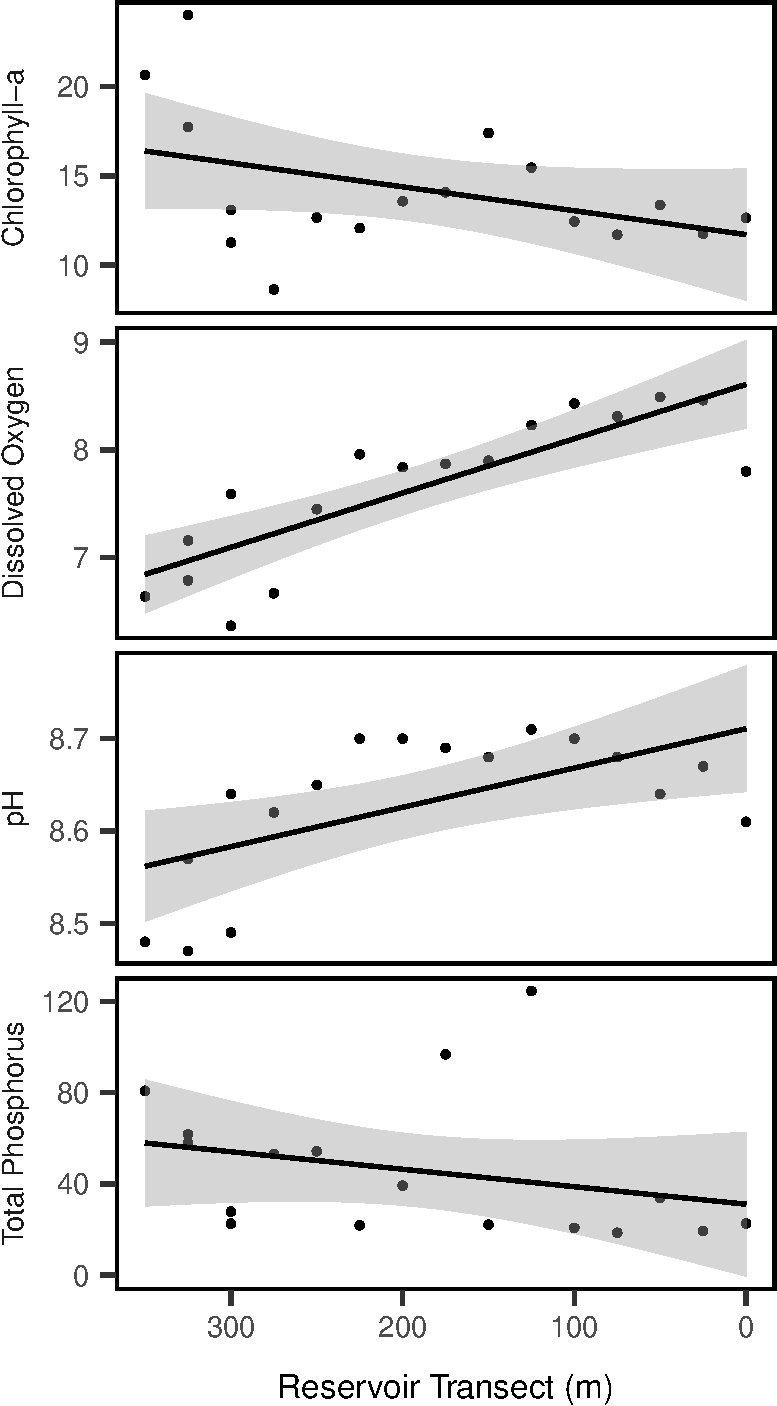
\includegraphics[width=0.7\linewidth]{ReservoirGradient_files/figure-latex/env_plot-1} \end{center}

So, there are some weak gradients, but nothing too prevailing.

\section{Analyze Diversity}\label{analyze-diversity}

Now, we will analyze the bacterial diversity in the reservoir and nearby
soils to figure out how well they support different mechanisms of
community assembly.

\subsection{\texorpdfstring{How does \(\alpha\)-diversity vary along the
reservoir?}{How does \textbackslash{}alpha-diversity vary along the reservoir?}}\label{how-does-alpha-diversity-vary-along-the-reservoir}

First, we use the method of rarefaction and extrapolation developed by
Chao et al. in the iNEXT package.

\begin{Shaded}
\begin{Highlighting}[]
\CommentTok{# Observed Richness}
\NormalTok{S.obs <-}\StringTok{ }\KeywordTok{rowSums}\NormalTok{((OTUs }\OperatorTok{>}\StringTok{ }\DecValTok{0}\NormalTok{) }\OperatorTok{*}\StringTok{ }\DecValTok{1}\NormalTok{)}

\CommentTok{# Simpson's Evenness}
\NormalTok{SimpE <-}\StringTok{ }\ControlFlowTok{function}\NormalTok{(}\DataTypeTok{x =} \StringTok{""}\NormalTok{)\{}
\NormalTok{  x <-}\StringTok{ }\KeywordTok{as.data.frame}\NormalTok{(x)}
\NormalTok{  D <-}\StringTok{ }\KeywordTok{diversity}\NormalTok{(x, }\StringTok{"inv"}\NormalTok{)}
\NormalTok{  S <-}\StringTok{ }\KeywordTok{sum}\NormalTok{((x }\OperatorTok{>}\StringTok{ }\DecValTok{0}\NormalTok{) }\OperatorTok{*}\StringTok{ }\DecValTok{1}\NormalTok{) }
\NormalTok{  E <-}\StringTok{ }\NormalTok{(D)}\OperatorTok{/}\NormalTok{S }
  \KeywordTok{return}\NormalTok{(E)}
\NormalTok{\}}
\NormalTok{simpsE <-}\StringTok{ }\KeywordTok{round}\NormalTok{(}\KeywordTok{apply}\NormalTok{(OTUs, }\DecValTok{1}\NormalTok{, SimpE), }\DecValTok{3}\NormalTok{)}
\NormalTok{shan <-}\StringTok{ }\KeywordTok{diversity}\NormalTok{(OTUs, }\DataTypeTok{index =} \StringTok{"shannon"}\NormalTok{)}
\NormalTok{exp.shan <-}\StringTok{ }\KeywordTok{exp}\NormalTok{(shan)}
\NormalTok{alpha.div <-}\StringTok{ }\KeywordTok{cbind}\NormalTok{(design, S.obs, simpsE, shan, exp.shan)}


\CommentTok{# # estimate asymptotic richness}
\CommentTok{# divestim <- iNEXT(t(OTUs), datatype = "abundance", nboot = 999)}
\CommentTok{# saveRDS(divestim, file = "intermediate-data/inext-output-999boots.rda")}
\NormalTok{divestim <-}\StringTok{ }\KeywordTok{read_rds}\NormalTok{(}\StringTok{"intermediate-data/inext-output-999boots.rda"}\NormalTok{)}
\NormalTok{divestim.df <-}\StringTok{ }\KeywordTok{fortify}\NormalTok{(divestim) }\OperatorTok\StringTok{ }
\StringTok{  }\KeywordTok{mutate}\NormalTok{(}\DataTypeTok{habitat =} \KeywordTok{str_to_title}\NormalTok{(design[}\KeywordTok{as.character}\NormalTok{(site),}\StringTok{"type"}\NormalTok{]))}

\NormalTok{divestim.df }\OperatorTok\StringTok{ }
\StringTok{  }\KeywordTok{ggplot}\NormalTok{(}\KeywordTok{aes}\NormalTok{(}\DataTypeTok{x =}\NormalTok{ x, }\DataTypeTok{y =}\NormalTok{ y, }
             \DataTypeTok{ymin =}\NormalTok{ y.lwr, }\DataTypeTok{ymax =}\NormalTok{ y.upr, }
             \DataTypeTok{color =}\NormalTok{ habitat, }\DataTypeTok{fill =}\NormalTok{ habitat, }\DataTypeTok{group =}\NormalTok{ site)) }\OperatorTok{+}
\StringTok{  }\KeywordTok{geom_ribbon}\NormalTok{(}\DataTypeTok{data=}\KeywordTok{subset}\NormalTok{(divestim.df, method }\OperatorTok{==}\StringTok{ "extrapolated"}\NormalTok{), }\DataTypeTok{alpha =} \FloatTok{0.3}\NormalTok{) }\OperatorTok{+}
\StringTok{  }\KeywordTok{geom_line}\NormalTok{(}\DataTypeTok{data=}\KeywordTok{subset}\NormalTok{(divestim.df, method }\OperatorTok{==}\StringTok{ "interpolated"}\NormalTok{), }\DataTypeTok{size =} \DecValTok{1}\NormalTok{, }\DataTypeTok{alpha =}\NormalTok{ .}\DecValTok{8}\NormalTok{) }\OperatorTok{+}
\StringTok{  }\KeywordTok{geom_line}\NormalTok{(}\DataTypeTok{alpha =} \DecValTok{1}\NormalTok{, }\DataTypeTok{linetype =} \StringTok{"dashed"}\NormalTok{) }\OperatorTok{+}
\StringTok{  }\KeywordTok{scale_x_continuous}\NormalTok{(}\DataTypeTok{labels =}\NormalTok{ scales}\OperatorTok{::}\NormalTok{comma) }\OperatorTok{+}
\StringTok{  }\KeywordTok{labs}\NormalTok{(}\DataTypeTok{x =} \StringTok{"Sample Size"}\NormalTok{, }\DataTypeTok{y =} \StringTok{"Species Diversity"}\NormalTok{) }\OperatorTok{+}
\StringTok{  }\KeywordTok{theme}\NormalTok{(}\DataTypeTok{legend.position =}  \KeywordTok{c}\NormalTok{(.}\DecValTok{9}\NormalTok{,.}\DecValTok{95}\NormalTok{)) }\OperatorTok{+}
\StringTok{  }\KeywordTok{scale_color_grey}\NormalTok{(}\DataTypeTok{end =}\NormalTok{ .}\DecValTok{7}\NormalTok{) }\OperatorTok{+}
\StringTok{  }\KeywordTok{scale_fill_grey}\NormalTok{(}\DataTypeTok{end =}\NormalTok{ .}\DecValTok{7}\NormalTok{)}
\end{Highlighting}
\end{Shaded}

\begin{center}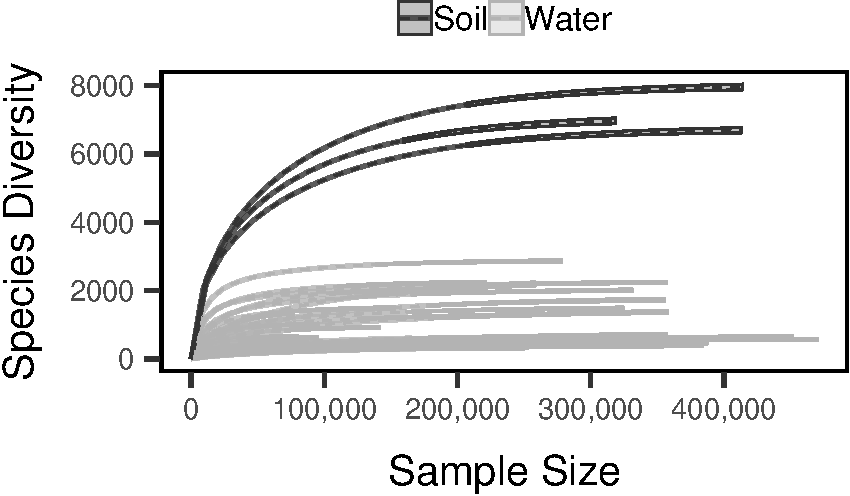
\includegraphics[width=0.7\linewidth]{ReservoirGradient_files/figure-latex/rarefaction-extrapolation-1} \end{center}

Next, we'll extract the estimates for the Hill numbers at different
levels of q, which differentially weight common versus rare species.

\begin{Shaded}
\begin{Highlighting}[]
\NormalTok{hill.estim <-}\StringTok{ }\NormalTok{divestim}\OperatorTok{$}\NormalTok{AsyEst }\OperatorTok\StringTok{ }\KeywordTok{filter}\NormalTok{(Diversity }\OperatorTok{==}\StringTok{ "Species richness"}\NormalTok{) }\OperatorTok\StringTok{ }
\StringTok{  }\KeywordTok{left_join}\NormalTok{(}\KeywordTok{rownames_to_column}\NormalTok{(alpha.div), }\DataTypeTok{by =} \KeywordTok{c}\NormalTok{(}\StringTok{"Observed"}\NormalTok{ =}\StringTok{ "S.obs"}\NormalTok{)) }\OperatorTok\StringTok{ }
\StringTok{  }\KeywordTok{select}\NormalTok{(Site, rowname, station, molecule, type, distance) }\OperatorTok\StringTok{ }
\StringTok{  }\KeywordTok{left_join}\NormalTok{(divestim}\OperatorTok{$}\NormalTok{AsyEst, }\DataTypeTok{by =} \StringTok{"Site"}\NormalTok{)}

\NormalTok{hill.water <-}\StringTok{ }\KeywordTok{as_tibble}\NormalTok{(hill.estim) }\OperatorTok\StringTok{ }\KeywordTok{filter}\NormalTok{(type }\OperatorTok{==}\StringTok{ "water"}\NormalTok{)}
\NormalTok{hill.water.rich <-}\StringTok{ }\KeywordTok{subset}\NormalTok{(hill.water, Diversity }\OperatorTok{==}\StringTok{ "Species richness"}\NormalTok{)}
\NormalTok{hill.water.shan <-}\StringTok{ }\KeywordTok{subset}\NormalTok{(hill.water, Diversity }\OperatorTok{==}\StringTok{ "Shannon diversity"}\NormalTok{)}
\NormalTok{hill.water.simp <-}\StringTok{ }\KeywordTok{subset}\NormalTok{(hill.water, Diversity }\OperatorTok{==}\StringTok{ "Simpson diversity"}\NormalTok{)}

\NormalTok{hill.water.mod.rich <-}\StringTok{ }\KeywordTok{lm}\NormalTok{(Estimator }\OperatorTok{~}\StringTok{ }\NormalTok{distance }\OperatorTok{*}\StringTok{ }\NormalTok{molecule, }\DataTypeTok{data =}\NormalTok{ hill.water.rich)}
\NormalTok{hill.water.mod.shan <-}\StringTok{ }\KeywordTok{lm}\NormalTok{(Estimator }\OperatorTok{~}\StringTok{ }\NormalTok{distance }\OperatorTok{*}\StringTok{ }\NormalTok{molecule, }\DataTypeTok{data =}\NormalTok{ hill.water.shan)}
\NormalTok{hill.water.mod.simp <-}\StringTok{ }\KeywordTok{lm}\NormalTok{(Estimator }\OperatorTok{~}\StringTok{ }\NormalTok{distance }\OperatorTok{*}\StringTok{ }\NormalTok{molecule, }\DataTypeTok{data =}\NormalTok{ hill.water.simp)}

\KeywordTok{summary}\NormalTok{(hill.water.mod.rich)}
\end{Highlighting}
\end{Shaded}

\begin{verbatim}
## 
## Call:
## lm(formula = Estimator ~ distance * molecule, data = hill.water.rich)
## 
## Residuals:
##     Min      1Q  Median      3Q     Max 
## -518.38 -137.60    0.71   98.61  718.25 
## 
## Coefficients:
##                      Estimate Std. Error t value Pr(>|t|)    
## (Intercept)          468.6274   128.2862   3.653 0.000918 ***
## distance               5.2143     0.5397   9.662 5.22e-11 ***
## moleculeRNA          104.9450   166.1694   0.632 0.532164    
## distance:moleculeRNA  -5.1222     0.7163  -7.151 4.07e-08 ***
## ---
## Signif. codes:  0 '***' 0.001 '**' 0.01 '*' 0.05 '.' 0.1 ' ' 1
## 
## Residual standard error: 258.7 on 32 degrees of freedom
## Multiple R-squared:  0.8714, Adjusted R-squared:  0.8593 
## F-statistic: 72.26 on 3 and 32 DF,  p-value: 2.431e-14
\end{verbatim}

\begin{Shaded}
\begin{Highlighting}[]
\KeywordTok{summary}\NormalTok{(hill.water.mod.shan)}
\end{Highlighting}
\end{Shaded}

\begin{verbatim}
## 
## Call:
## lm(formula = Estimator ~ distance * molecule, data = hill.water.shan)
## 
## Residuals:
##      Min       1Q   Median       3Q      Max 
## -123.915  -14.841   -3.500    6.902  157.964 
## 
## Coefficients:
##                      Estimate Std. Error t value Pr(>|t|)   
## (Intercept)           55.5031    24.9703   2.223  0.03342 * 
## distance               0.2892     0.1050   2.753  0.00965 **
## moleculeRNA          -35.5144    32.3441  -1.098  0.28039   
## distance:moleculeRNA  -0.2905     0.1394  -2.084  0.04525 * 
## ---
## Signif. codes:  0 '***' 0.001 '**' 0.01 '*' 0.05 '.' 0.1 ' ' 1
## 
## Residual standard error: 50.35 on 32 degrees of freedom
## Multiple R-squared:  0.5556, Adjusted R-squared:  0.514 
## F-statistic: 13.34 on 3 and 32 DF,  p-value: 8.138e-06
\end{verbatim}

\begin{Shaded}
\begin{Highlighting}[]
\KeywordTok{summary}\NormalTok{(hill.water.mod.simp)}
\end{Highlighting}
\end{Shaded}

\begin{verbatim}
## 
## Call:
## lm(formula = Estimator ~ distance * molecule, data = hill.water.simp)
## 
## Residuals:
##     Min      1Q  Median      3Q     Max 
## -41.589  -7.222  -0.977   6.321  39.440 
## 
## Coefficients:
##                       Estimate Std. Error t value Pr(>|t|)    
## (Intercept)           31.61377    7.45207   4.242 0.000176 ***
## distance               0.05218    0.03135   1.664 0.105804    
## moleculeRNA          -22.18812    9.65268  -2.299 0.028205 *  
## distance:moleculeRNA  -0.04408    0.04161  -1.059 0.297369    
## ---
## Signif. codes:  0 '***' 0.001 '**' 0.01 '*' 0.05 '.' 0.1 ' ' 1
## 
## Residual standard error: 15.02 on 32 degrees of freedom
## Multiple R-squared:  0.5693, Adjusted R-squared:  0.529 
## F-statistic:  14.1 on 3 and 32 DF,  p-value: 4.985e-06
\end{verbatim}

\begin{Shaded}
\begin{Highlighting}[]
\NormalTok{hill.water.mods <-}\StringTok{ }\KeywordTok{as_tibble}\NormalTok{(}\KeywordTok{rbind.data.frame}\NormalTok{(}
  \KeywordTok{tidy}\NormalTok{(hill.water.mod.rich) }\OperatorTok\StringTok{ }\KeywordTok{add_column}\NormalTok{(}\DataTypeTok{Diversity =} \StringTok{"Species richness"}\NormalTok{),}
  \KeywordTok{tidy}\NormalTok{(hill.water.mod.shan) }\OperatorTok\StringTok{ }\KeywordTok{add_column}\NormalTok{(}\DataTypeTok{Diversity =} \StringTok{"Shannon diversity"}\NormalTok{),}
  \KeywordTok{tidy}\NormalTok{(hill.water.mod.simp) }\OperatorTok\StringTok{ }\KeywordTok{add_column}\NormalTok{(}\DataTypeTok{Diversity =} \StringTok{"Simpson diversity"}\NormalTok{)}
\NormalTok{))}

\CommentTok{# Summary table of the model results. }
\NormalTok{hill.water.mods }\OperatorTok\StringTok{ }
\StringTok{  }\KeywordTok{group_by}\NormalTok{(Diversity) }\OperatorTok\StringTok{ }
\StringTok{  }\KeywordTok{rename}\NormalTok{(}\StringTok{"Term"}\NormalTok{ =}\StringTok{ }\NormalTok{term, }
         \StringTok{"Estimate"}\NormalTok{ =}\StringTok{ }\NormalTok{estimate, }
         \StringTok{"Std. Error"}\NormalTok{ =}\StringTok{ }\NormalTok{std.error, }
         \StringTok{"Statistic"}\NormalTok{ =}\StringTok{ }\NormalTok{statistic, }
         \StringTok{"p-value"}\NormalTok{ =}\StringTok{ }\NormalTok{p.value) }\OperatorTok\StringTok{ }
\StringTok{  }\KeywordTok{filter}\NormalTok{(Term }\OperatorTok{!=}\StringTok{ "(Intercept)"}\NormalTok{) }\OperatorTok\StringTok{ }
\StringTok{  }\KeywordTok{select}\NormalTok{(Diversity, }\KeywordTok{everything}\NormalTok{()) }\OperatorTok\StringTok{ }
\StringTok{  }\KeywordTok{mutate_if}\NormalTok{(is.double, signif, }\DataTypeTok{digits =} \DecValTok{3}\NormalTok{) }\OperatorTok\StringTok{ }
\StringTok{  }\KeywordTok{pander}\NormalTok{()}
\end{Highlighting}
\end{Shaded}

\begin{longtable}[]{@{}ccccc@{}}
\caption{Table continues below}\tabularnewline
\toprule
\begin{minipage}[b]{0.21\columnwidth}\centering\strut
Diversity\strut
\end{minipage} & \begin{minipage}[b]{0.25\columnwidth}\centering\strut
Term\strut
\end{minipage} & \begin{minipage}[b]{0.12\columnwidth}\centering\strut
Estimate\strut
\end{minipage} & \begin{minipage}[b]{0.14\columnwidth}\centering\strut
Std. Error\strut
\end{minipage} & \begin{minipage}[b]{0.14\columnwidth}\centering\strut
Statistic\strut
\end{minipage}\tabularnewline
\midrule
\endfirsthead
\toprule
\begin{minipage}[b]{0.21\columnwidth}\centering\strut
Diversity\strut
\end{minipage} & \begin{minipage}[b]{0.25\columnwidth}\centering\strut
Term\strut
\end{minipage} & \begin{minipage}[b]{0.12\columnwidth}\centering\strut
Estimate\strut
\end{minipage} & \begin{minipage}[b]{0.14\columnwidth}\centering\strut
Std. Error\strut
\end{minipage} & \begin{minipage}[b]{0.14\columnwidth}\centering\strut
Statistic\strut
\end{minipage}\tabularnewline
\midrule
\endhead
\begin{minipage}[t]{0.21\columnwidth}\centering\strut
Species richness\strut
\end{minipage} & \begin{minipage}[t]{0.25\columnwidth}\centering\strut
distance\strut
\end{minipage} & \begin{minipage}[t]{0.12\columnwidth}\centering\strut
5.21\strut
\end{minipage} & \begin{minipage}[t]{0.14\columnwidth}\centering\strut
0.54\strut
\end{minipage} & \begin{minipage}[t]{0.14\columnwidth}\centering\strut
9.66\strut
\end{minipage}\tabularnewline
\begin{minipage}[t]{0.21\columnwidth}\centering\strut
Species richness\strut
\end{minipage} & \begin{minipage}[t]{0.25\columnwidth}\centering\strut
moleculeRNA\strut
\end{minipage} & \begin{minipage}[t]{0.12\columnwidth}\centering\strut
105\strut
\end{minipage} & \begin{minipage}[t]{0.14\columnwidth}\centering\strut
166\strut
\end{minipage} & \begin{minipage}[t]{0.14\columnwidth}\centering\strut
0.632\strut
\end{minipage}\tabularnewline
\begin{minipage}[t]{0.21\columnwidth}\centering\strut
Species richness\strut
\end{minipage} & \begin{minipage}[t]{0.25\columnwidth}\centering\strut
distance:moleculeRNA\strut
\end{minipage} & \begin{minipage}[t]{0.12\columnwidth}\centering\strut
-5.12\strut
\end{minipage} & \begin{minipage}[t]{0.14\columnwidth}\centering\strut
0.716\strut
\end{minipage} & \begin{minipage}[t]{0.14\columnwidth}\centering\strut
-7.15\strut
\end{minipage}\tabularnewline
\begin{minipage}[t]{0.21\columnwidth}\centering\strut
Shannon diversity\strut
\end{minipage} & \begin{minipage}[t]{0.25\columnwidth}\centering\strut
distance\strut
\end{minipage} & \begin{minipage}[t]{0.12\columnwidth}\centering\strut
0.289\strut
\end{minipage} & \begin{minipage}[t]{0.14\columnwidth}\centering\strut
0.105\strut
\end{minipage} & \begin{minipage}[t]{0.14\columnwidth}\centering\strut
2.75\strut
\end{minipage}\tabularnewline
\begin{minipage}[t]{0.21\columnwidth}\centering\strut
Shannon diversity\strut
\end{minipage} & \begin{minipage}[t]{0.25\columnwidth}\centering\strut
moleculeRNA\strut
\end{minipage} & \begin{minipage}[t]{0.12\columnwidth}\centering\strut
-35.5\strut
\end{minipage} & \begin{minipage}[t]{0.14\columnwidth}\centering\strut
32.3\strut
\end{minipage} & \begin{minipage}[t]{0.14\columnwidth}\centering\strut
-1.1\strut
\end{minipage}\tabularnewline
\begin{minipage}[t]{0.21\columnwidth}\centering\strut
Shannon diversity\strut
\end{minipage} & \begin{minipage}[t]{0.25\columnwidth}\centering\strut
distance:moleculeRNA\strut
\end{minipage} & \begin{minipage}[t]{0.12\columnwidth}\centering\strut
-0.291\strut
\end{minipage} & \begin{minipage}[t]{0.14\columnwidth}\centering\strut
0.139\strut
\end{minipage} & \begin{minipage}[t]{0.14\columnwidth}\centering\strut
-2.08\strut
\end{minipage}\tabularnewline
\begin{minipage}[t]{0.21\columnwidth}\centering\strut
Simpson diversity\strut
\end{minipage} & \begin{minipage}[t]{0.25\columnwidth}\centering\strut
distance\strut
\end{minipage} & \begin{minipage}[t]{0.12\columnwidth}\centering\strut
0.0522\strut
\end{minipage} & \begin{minipage}[t]{0.14\columnwidth}\centering\strut
0.0313\strut
\end{minipage} & \begin{minipage}[t]{0.14\columnwidth}\centering\strut
1.66\strut
\end{minipage}\tabularnewline
\begin{minipage}[t]{0.21\columnwidth}\centering\strut
Simpson diversity\strut
\end{minipage} & \begin{minipage}[t]{0.25\columnwidth}\centering\strut
moleculeRNA\strut
\end{minipage} & \begin{minipage}[t]{0.12\columnwidth}\centering\strut
-22.2\strut
\end{minipage} & \begin{minipage}[t]{0.14\columnwidth}\centering\strut
9.65\strut
\end{minipage} & \begin{minipage}[t]{0.14\columnwidth}\centering\strut
-2.3\strut
\end{minipage}\tabularnewline
\begin{minipage}[t]{0.21\columnwidth}\centering\strut
Simpson diversity\strut
\end{minipage} & \begin{minipage}[t]{0.25\columnwidth}\centering\strut
distance:moleculeRNA\strut
\end{minipage} & \begin{minipage}[t]{0.12\columnwidth}\centering\strut
-0.0441\strut
\end{minipage} & \begin{minipage}[t]{0.14\columnwidth}\centering\strut
0.0416\strut
\end{minipage} & \begin{minipage}[t]{0.14\columnwidth}\centering\strut
-1.06\strut
\end{minipage}\tabularnewline
\bottomrule
\end{longtable}

\begin{longtable}[]{@{}c@{}}
\toprule
\begin{minipage}[b]{0.13\columnwidth}\centering\strut
p-value\strut
\end{minipage}\tabularnewline
\midrule
\endhead
\begin{minipage}[t]{0.13\columnwidth}\centering\strut
5.22e-11\strut
\end{minipage}\tabularnewline
\begin{minipage}[t]{0.13\columnwidth}\centering\strut
0.532\strut
\end{minipage}\tabularnewline
\begin{minipage}[t]{0.13\columnwidth}\centering\strut
4.07e-08\strut
\end{minipage}\tabularnewline
\begin{minipage}[t]{0.13\columnwidth}\centering\strut
0.00965\strut
\end{minipage}\tabularnewline
\begin{minipage}[t]{0.13\columnwidth}\centering\strut
0.28\strut
\end{minipage}\tabularnewline
\begin{minipage}[t]{0.13\columnwidth}\centering\strut
0.0453\strut
\end{minipage}\tabularnewline
\begin{minipage}[t]{0.13\columnwidth}\centering\strut
0.106\strut
\end{minipage}\tabularnewline
\begin{minipage}[t]{0.13\columnwidth}\centering\strut
0.0282\strut
\end{minipage}\tabularnewline
\begin{minipage}[t]{0.13\columnwidth}\centering\strut
0.297\strut
\end{minipage}\tabularnewline
\bottomrule
\end{longtable}

\begin{Shaded}
\begin{Highlighting}[]
\NormalTok{hill.estim }\OperatorTok\StringTok{ }\KeywordTok{filter}\NormalTok{(type }\OperatorTok{==}\StringTok{ "water"}\NormalTok{) }\OperatorTok\StringTok{ }
\StringTok{  }\KeywordTok{mutate}\NormalTok{(}\DataTypeTok{molecule =} \KeywordTok{ifelse}\NormalTok{(molecule }\OperatorTok{==}\StringTok{ "DNA"}\NormalTok{, }\StringTok{"Total"}\NormalTok{, }\StringTok{"Active"}\NormalTok{)) }\OperatorTok\StringTok{ }
\StringTok{  }\KeywordTok{ggplot}\NormalTok{(}\KeywordTok{aes}\NormalTok{(}\DataTypeTok{x =}\NormalTok{ distance, }\DataTypeTok{y =}\NormalTok{ Estimator, }
             \DataTypeTok{ymin =}\NormalTok{ LCL, }\DataTypeTok{ymax =}\NormalTok{ UCL,}
             \DataTypeTok{color =}\NormalTok{ molecule, }\DataTypeTok{fill =}\NormalTok{ molecule, }\DataTypeTok{shape =}\NormalTok{ molecule)) }\OperatorTok{+}\StringTok{ }
\StringTok{  }\KeywordTok{geom_point}\NormalTok{(}\DataTypeTok{size =}\DecValTok{3}\NormalTok{) }\OperatorTok{+}\StringTok{ }
\StringTok{  }\CommentTok{# geom_errorbar(size = .5, aes(ymin = Estimator - s.e., ymax = Estimator + s.e.), }
\StringTok{  }\CommentTok{#                width = 10, alpha = 0.5) +}
\StringTok{  }\KeywordTok{geom_smooth}\NormalTok{(}\DataTypeTok{method =} \StringTok{"lm"}\NormalTok{, }\KeywordTok{aes}\NormalTok{(}\DataTypeTok{linetype =}\NormalTok{ molecule)) }\OperatorTok{+}
\StringTok{  }\KeywordTok{labs}\NormalTok{(}\DataTypeTok{x =} \StringTok{"Reservoir Transect (m)"}\NormalTok{,}
       \DataTypeTok{y =} \StringTok{"Estimated Diversity (Hill Numbers)"}\NormalTok{) }\OperatorTok{+}
\StringTok{  }\KeywordTok{scale_color_manual}\NormalTok{(}\DataTypeTok{values =}\NormalTok{ my.cols) }\OperatorTok{+}
\StringTok{  }\KeywordTok{scale_fill_manual}\NormalTok{(}\DataTypeTok{values =}\NormalTok{ my.cols) }\OperatorTok{+}\StringTok{ }
\StringTok{  }\KeywordTok{theme}\NormalTok{(}\DataTypeTok{legend.position =} \KeywordTok{c}\NormalTok{(.}\DecValTok{85}\NormalTok{,.}\DecValTok{95}\NormalTok{)) }\OperatorTok{+}
\StringTok{  }\KeywordTok{scale_x_reverse}\NormalTok{() }\OperatorTok{+}
\StringTok{  }\KeywordTok{facet_grid}\NormalTok{(Diversity }\OperatorTok{~}\StringTok{ }\NormalTok{., }\DataTypeTok{scales =} \StringTok{"free"}\NormalTok{)}
\end{Highlighting}
\end{Shaded}

\begin{center}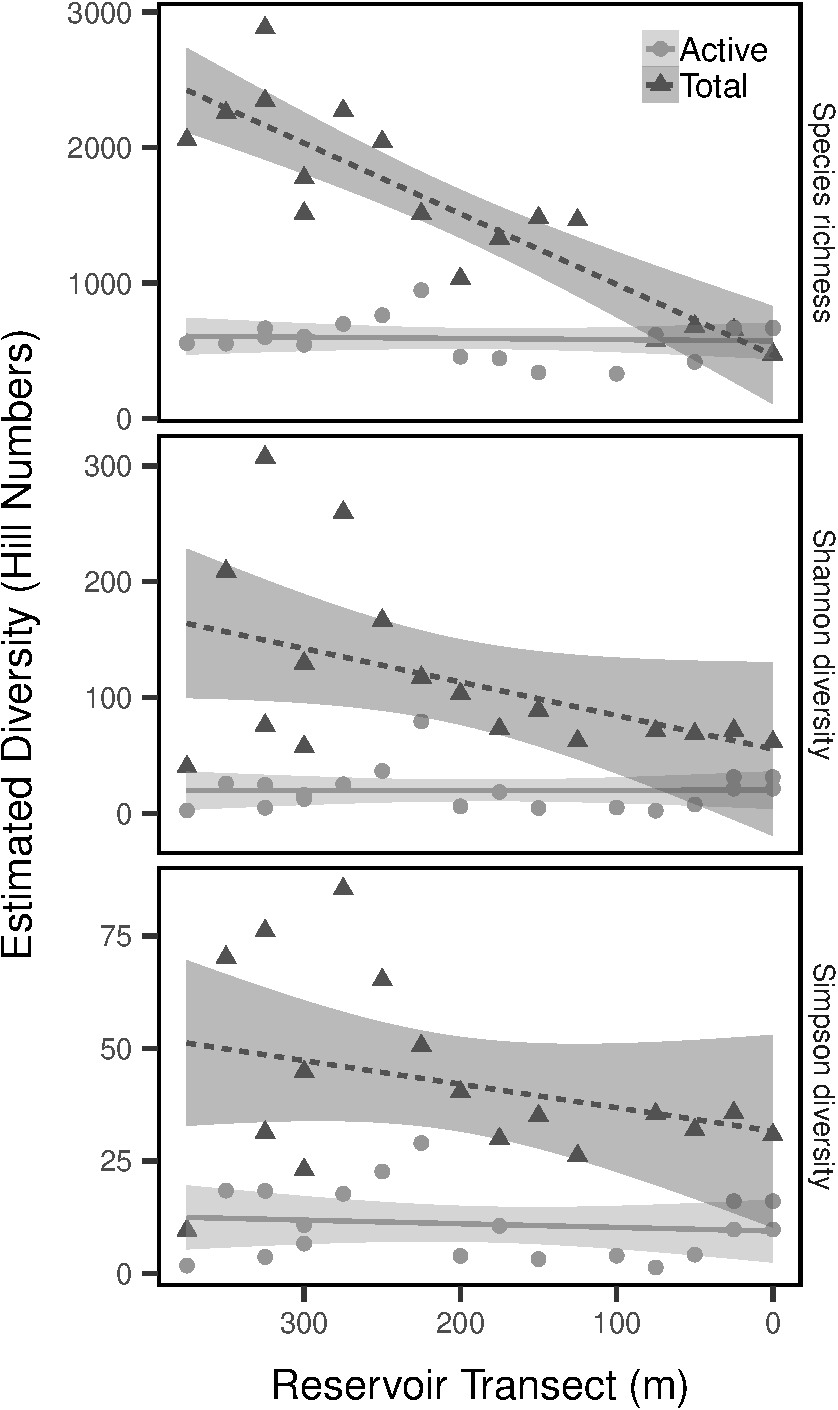
\includegraphics[width=0.7\linewidth]{ReservoirGradient_files/figure-latex/hill_numbers-1} \end{center}

So, from the basis of these results, we can make the following
conclusions. First, we note that diversity in the total community decays
from the stream inlet to the dam of the reservoir. That is, all the
lines have a negative slope. However, we do not see this decay in the
metabolically active community. Second, we note that the metabolically
actively community has much lower diversity than the total community
near the soils, but this difference decreases toward the dam. Last,
because we quantified diversity across three orders of Hill numbers (q =
0, 1, and 2), we can also say something about the relative importance of
rare versus common taxa along the reservoir transect. We see the the
significance of the distance-by-molecule interaction term decrease as
rare taxa are downweighted in favor of common taxa. This suggests that
the differences between the active and total communities along the
transect is driven primarily by rare taxa. However, the general trend of
higher Simpson diversity across the whole transect suggests that
low-activity, but relatively common, taxa are maintained in the
reservoir.

\subsection{How does community structure change along the
gradient?}\label{how-does-community-structure-change-along-the-gradient}

First, we'll just get an overview of how the communities look along the
aquatic transect.

\begin{Shaded}
\begin{Highlighting}[]
\NormalTok{ul.pcoa <-}\StringTok{ }\KeywordTok{cmdscale}\NormalTok{(}\KeywordTok{vegdist}\NormalTok{(OTUsREL.log, }\DataTypeTok{method=}\StringTok{"bray"}\NormalTok{), }\DecValTok{2}\NormalTok{, }\DataTypeTok{eig =}\NormalTok{ T, }\DataTypeTok{add =}\NormalTok{ T)}
\NormalTok{explainvars <-}\StringTok{ }\KeywordTok{round}\NormalTok{(}\KeywordTok{eigenvals}\NormalTok{(ul.pcoa)[}\KeywordTok{c}\NormalTok{(}\DecValTok{1}\NormalTok{,}\DecValTok{2}\NormalTok{)]}\OperatorTok{/}\KeywordTok{sum}\NormalTok{(}\KeywordTok{eigenvals}\NormalTok{(ul.pcoa)),}\DecValTok{3}\NormalTok{) }\OperatorTok{*}\DecValTok{100}
\NormalTok{water.pcvals <-}\StringTok{ }\KeywordTok{data.frame}\NormalTok{(}\KeywordTok{scores}\NormalTok{(ul.pcoa)) }\OperatorTok\StringTok{ }
\StringTok{  }\KeywordTok{rownames_to_column}\NormalTok{(}\StringTok{"name"}\NormalTok{) }\OperatorTok\StringTok{ }
\StringTok{  }\KeywordTok{left_join}\NormalTok{(}\KeywordTok{rownames_to_column}\NormalTok{(design, }\StringTok{"name"}\NormalTok{)) }\OperatorTok\StringTok{ }
\StringTok{  }\KeywordTok{arrange}\NormalTok{(}\KeywordTok{desc}\NormalTok{(distance)) }\OperatorTok\StringTok{ }\KeywordTok{filter}\NormalTok{(type }\OperatorTok{==}\StringTok{ "water"}\NormalTok{)}
\NormalTok{pc_dists <-}\StringTok{ }\KeywordTok{tibble}\NormalTok{(}
  \DataTypeTok{DNA_dim1 =} \KeywordTok{subset}\NormalTok{(water.pcvals, molecule }\OperatorTok{==}\StringTok{ "DNA"}\NormalTok{)}\OperatorTok{$}\NormalTok{Dim1,}
  \DataTypeTok{DNA_dim2 =} \KeywordTok{subset}\NormalTok{(water.pcvals, molecule }\OperatorTok{==}\StringTok{ "DNA"}\NormalTok{)}\OperatorTok{$}\NormalTok{Dim2,}
  \DataTypeTok{RNA_dim1 =} \KeywordTok{subset}\NormalTok{(water.pcvals, molecule }\OperatorTok{==}\StringTok{ "RNA"}\NormalTok{)}\OperatorTok{$}\NormalTok{Dim1,}
  \DataTypeTok{RNA_dim2 =} \KeywordTok{subset}\NormalTok{(water.pcvals, molecule }\OperatorTok{==}\StringTok{ "RNA"}\NormalTok{)}\OperatorTok{$}\NormalTok{Dim2)}
\KeywordTok{data.frame}\NormalTok{(}\KeywordTok{scores}\NormalTok{(ul.pcoa)) }\OperatorTok\StringTok{ }
\StringTok{  }\KeywordTok{rownames_to_column}\NormalTok{(}\StringTok{"name"}\NormalTok{) }\OperatorTok\StringTok{ }
\StringTok{  }\KeywordTok{left_join}\NormalTok{(}\KeywordTok{rownames_to_column}\NormalTok{(design, }\StringTok{"name"}\NormalTok{)) }\OperatorTok\StringTok{ }
\StringTok{  }\KeywordTok{arrange}\NormalTok{(}\KeywordTok{desc}\NormalTok{(distance)) }\OperatorTok\StringTok{ }\KeywordTok{filter}\NormalTok{(type }\OperatorTok{==}\StringTok{ "water"}\NormalTok{) }\OperatorTok\StringTok{ }
\StringTok{  }\KeywordTok{mutate}\NormalTok{(}\DataTypeTok{molecule =} \KeywordTok{ifelse}\NormalTok{(molecule }\OperatorTok{==}\StringTok{ "DNA"}\NormalTok{, }\StringTok{"Total"}\NormalTok{, }\StringTok{"Active"}\NormalTok{)) }\OperatorTok\StringTok{ }
\StringTok{  }\KeywordTok{ggplot}\NormalTok{(}\KeywordTok{aes}\NormalTok{(}\DataTypeTok{x =}\NormalTok{ Dim1, }\DataTypeTok{y =}\NormalTok{ Dim2)) }\OperatorTok{+}
\StringTok{  }\KeywordTok{geom_point}\NormalTok{(}\DataTypeTok{size =} \DecValTok{3}\NormalTok{, }\DataTypeTok{alpha =} \FloatTok{0.5}\NormalTok{, }\KeywordTok{aes}\NormalTok{(}\DataTypeTok{color =}\NormalTok{ molecule, }\DataTypeTok{shape =}\NormalTok{ molecule)) }\OperatorTok{+}\StringTok{ }
\StringTok{  }\KeywordTok{geom_path}\NormalTok{(}\DataTypeTok{size =} \FloatTok{1.2}\NormalTok{, }\DataTypeTok{alpha =} \FloatTok{0.75}\NormalTok{, }\DataTypeTok{arrow =} \KeywordTok{arrow}\NormalTok{(}\DataTypeTok{angle =} \DecValTok{20}\NormalTok{,}
                          \DataTypeTok{length =} \KeywordTok{unit}\NormalTok{(}\FloatTok{0.35}\NormalTok{, }\StringTok{"cm"}\NormalTok{),}
                          \DataTypeTok{type =} \StringTok{"closed"}\NormalTok{), }\KeywordTok{aes}\NormalTok{(}\DataTypeTok{color =}\NormalTok{ molecule, }\DataTypeTok{linetype =}\NormalTok{ molecule)) }\OperatorTok{+}
\StringTok{  }\KeywordTok{scale_color_manual}\NormalTok{(}\StringTok{"Community Subset"}\NormalTok{, }\DataTypeTok{values =}\NormalTok{ my.cols) }\OperatorTok{+}
\StringTok{  }\KeywordTok{geom_segment}\NormalTok{(}\DataTypeTok{data =}\NormalTok{ pc_dists,}
               \KeywordTok{aes}\NormalTok{(}\DataTypeTok{x =}\NormalTok{ DNA_dim1, }\DataTypeTok{y =}\NormalTok{ DNA_dim2,}
                   \DataTypeTok{xend =}\NormalTok{ RNA_dim1, }\DataTypeTok{yend =}\NormalTok{ RNA_dim2),}
               \DataTypeTok{alpha =} \DecValTok{0}\NormalTok{) }\OperatorTok{+}
\StringTok{  }\KeywordTok{coord_fixed}\NormalTok{() }\OperatorTok{+}
\StringTok{  }\KeywordTok{labs}\NormalTok{(}\DataTypeTok{x =} \KeywordTok{paste0}\NormalTok{(}\StringTok{"PCoA 1 ("}\NormalTok{, explainvars[}\DecValTok{1}\NormalTok{],}\StringTok{"%)"}\NormalTok{),}
       \DataTypeTok{y =} \KeywordTok{paste0}\NormalTok{(}\StringTok{"PCoA 2 ("}\NormalTok{, explainvars[}\DecValTok{2}\NormalTok{],}\StringTok{"%)"}\NormalTok{)) }\OperatorTok{+}
\StringTok{  }\KeywordTok{theme}\NormalTok{(}\DataTypeTok{legend.position =} \StringTok{"none"}\NormalTok{) }\OperatorTok{+}
\StringTok{  }\KeywordTok{annotate}\NormalTok{(}\DataTypeTok{geom =} \StringTok{"text"}\NormalTok{, }\DataTypeTok{x =}\NormalTok{ .}\DecValTok{2}\NormalTok{, }\DataTypeTok{y =} \OperatorTok{-}\NormalTok{.}\DecValTok{3}\NormalTok{, }\DataTypeTok{label =} \StringTok{"Active"}\NormalTok{, }\DataTypeTok{size =} \DecValTok{6}\NormalTok{) }\OperatorTok{+}
\StringTok{  }\KeywordTok{annotate}\NormalTok{(}\DataTypeTok{geom =} \StringTok{"text"}\NormalTok{, }\DataTypeTok{x =} \OperatorTok{-}\NormalTok{.}\DecValTok{3}\NormalTok{, }\DataTypeTok{y =}\NormalTok{ .}\DecValTok{1}\NormalTok{, }\DataTypeTok{label =} \StringTok{"Total"}\NormalTok{, }\DataTypeTok{size =} \DecValTok{6}\NormalTok{) }\OperatorTok{+}
\StringTok{  }\KeywordTok{ggsave}\NormalTok{(}\StringTok{"figures/active-tot-pcoa-trajectories.pdf"}\NormalTok{, }\DataTypeTok{bg =} \StringTok{"white"}\NormalTok{, }\DataTypeTok{width =} \DecValTok{8}\NormalTok{, }\DataTypeTok{height =} \DecValTok{8}\NormalTok{) }\OperatorTok{+}
\StringTok{  }\KeywordTok{ggsave}\NormalTok{(}\StringTok{"figures/active-tot-pcoa-trajectories.png"}\NormalTok{, }\DataTypeTok{width =} \DecValTok{8}\NormalTok{, }\DataTypeTok{height =} \DecValTok{8}\NormalTok{)}
\end{Highlighting}
\end{Shaded}

\begin{center}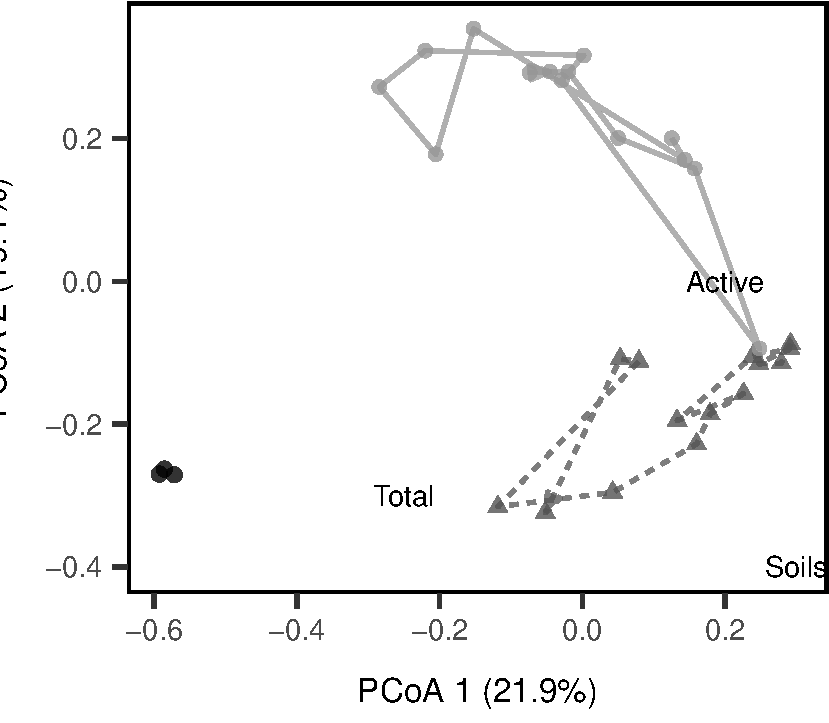
\includegraphics[width=0.7\linewidth]{ReservoirGradient_files/figure-latex/ordination-1} \end{center}

\begin{Shaded}
\begin{Highlighting}[]
\CommentTok{# animation}
\CommentTok{# traj.animate <- data.frame(scores(ul.pcoa)) %>% }
\CommentTok{#   rownames_to_column("name") %>% }
\CommentTok{#   left_join(rownames_to_column(design, "name")) %>% }
\CommentTok{#   arrange(desc(distance)) %>% filter(type == "water", station != "UL17", station != "UL18") %>% }
\CommentTok{#   mutate(molecule = ifelse(molecule == "DNA", "Total", "Active")) %>% }
\CommentTok{#   mutate(transect = desc(distance)) %>% }
\CommentTok{#   ggplot(aes(x = Dim1, y = Dim2, frame = transect, cumulative = TRUE)) +}
\CommentTok{#   geom_point(alpha = 0.75, size = 10, aes(color = molecule)) + }
\CommentTok{#   geom_path(alpha = 1, size = 1, arrow = arrow(angle = 20,}
\CommentTok{#                           length = unit(0.35, "cm"),}
\CommentTok{#                           type = "closed"), aes(color = molecule)) +}
\CommentTok{#   scale_color_manual(values = my.cols) +}
\CommentTok{#   theme(legend.title = element_blank()) +}
\CommentTok{#   coord_fixed() +}
\CommentTok{#   labs(x = paste0("PCoA 1 (", explainvars[1],"%)"),}
\CommentTok{#        y = paste0("PCoA 2 (", explainvars[2],"%)"))}
\CommentTok{# }
\CommentTok{# gganimate(traj.animate, filename = "../figures/trajectory-animation.mp4", ani.width = 800, ani.height = 800)}
\end{Highlighting}
\end{Shaded}

So, it appears that there is convergence in community structure along
the path from stream inlet to the dam. This could reflect a loss of
soil-derived taxa in the aquatic samples. To test this, we'll look at
\(\beta\)-diversity along the gradient with respect to the soil samples.
If we see a decay in similarity to soils, this suggests soil taxa are
having a comparatively lower influence with distance from the inlet.

\subsection{Similarity To Terrestrial Habitat Across Gradient
(Terrestrial
Influence)}\label{similarity-to-terrestrial-habitat-across-gradient-terrestrial-influence}

\begin{Shaded}
\begin{Highlighting}[]
\CommentTok{# Similarity to Soil Sample}
\NormalTok{UL.bray      <-}\StringTok{ }\DecValTok{1}\OperatorTok{-}\KeywordTok{as.matrix}\NormalTok{(}\KeywordTok{vegdist}\NormalTok{(OTUsREL.log, }\DataTypeTok{method=}\StringTok{"bray"}\NormalTok{))}
\NormalTok{UL.bray.lake <-}\StringTok{ }\NormalTok{UL.bray[}\OperatorTok{-}\KeywordTok{c}\NormalTok{(}\DecValTok{1}\OperatorTok{:}\DecValTok{3}\NormalTok{), }\DecValTok{1}\OperatorTok{:}\DecValTok{3}\NormalTok{] }
\NormalTok{bray.mean    <-}\StringTok{ }\KeywordTok{round}\NormalTok{(}\KeywordTok{apply}\NormalTok{(UL.bray.lake, }\DecValTok{1}\NormalTok{, mean), }\DecValTok{3}\NormalTok{)}
\NormalTok{bray.se      <-}\StringTok{ }\KeywordTok{round}\NormalTok{(}\KeywordTok{apply}\NormalTok{(UL.bray.lake, }\DecValTok{1}\NormalTok{, se), }\DecValTok{3}\NormalTok{)}
\NormalTok{UL.sim       <-}\StringTok{ }\KeywordTok{cbind}\NormalTok{(design[}\OperatorTok{-}\KeywordTok{c}\NormalTok{(}\DecValTok{1}\OperatorTok{:}\DecValTok{3}\NormalTok{), ], bray.mean, bray.se)}

\CommentTok{# Calculate Linear Model}
\NormalTok{model.terr <-}\StringTok{ }\KeywordTok{lm}\NormalTok{(bray.mean }\OperatorTok{~}\StringTok{ }\NormalTok{distance }\OperatorTok{*}\StringTok{ }\NormalTok{molecule, }\DataTypeTok{data =}\NormalTok{ UL.sim)}
\KeywordTok{pander}\NormalTok{(model.terr)}
\end{Highlighting}
\end{Shaded}

\begin{longtable}[]{@{}ccccc@{}}
\caption{Fitting linear model: bray.mean \textasciitilde{} distance *
molecule}\tabularnewline
\toprule
\begin{minipage}[b]{0.31\columnwidth}\centering\strut
~\strut
\end{minipage} & \begin{minipage}[b]{0.15\columnwidth}\centering\strut
Estimate\strut
\end{minipage} & \begin{minipage}[b]{0.15\columnwidth}\centering\strut
Std. Error\strut
\end{minipage} & \begin{minipage}[b]{0.12\columnwidth}\centering\strut
t value\strut
\end{minipage} & \begin{minipage}[b]{0.13\columnwidth}\centering\strut
Pr(\textgreater{}\textbar{}t\textbar{})\strut
\end{minipage}\tabularnewline
\midrule
\endfirsthead
\toprule
\begin{minipage}[b]{0.31\columnwidth}\centering\strut
~\strut
\end{minipage} & \begin{minipage}[b]{0.15\columnwidth}\centering\strut
Estimate\strut
\end{minipage} & \begin{minipage}[b]{0.15\columnwidth}\centering\strut
Std. Error\strut
\end{minipage} & \begin{minipage}[b]{0.12\columnwidth}\centering\strut
t value\strut
\end{minipage} & \begin{minipage}[b]{0.13\columnwidth}\centering\strut
Pr(\textgreater{}\textbar{}t\textbar{})\strut
\end{minipage}\tabularnewline
\midrule
\endhead
\begin{minipage}[t]{0.31\columnwidth}\centering\strut
\textbf{(Intercept)}\strut
\end{minipage} & \begin{minipage}[t]{0.15\columnwidth}\centering\strut
0.01524\strut
\end{minipage} & \begin{minipage}[t]{0.15\columnwidth}\centering\strut
0.01623\strut
\end{minipage} & \begin{minipage}[t]{0.12\columnwidth}\centering\strut
0.9392\strut
\end{minipage} & \begin{minipage}[t]{0.13\columnwidth}\centering\strut
0.3551\strut
\end{minipage}\tabularnewline
\begin{minipage}[t]{0.31\columnwidth}\centering\strut
\textbf{distance}\strut
\end{minipage} & \begin{minipage}[t]{0.15\columnwidth}\centering\strut
0.0004564\strut
\end{minipage} & \begin{minipage}[t]{0.15\columnwidth}\centering\strut
6.828e-05\strut
\end{minipage} & \begin{minipage}[t]{0.12\columnwidth}\centering\strut
6.684\strut
\end{minipage} & \begin{minipage}[t]{0.13\columnwidth}\centering\strut
2.097e-07\strut
\end{minipage}\tabularnewline
\begin{minipage}[t]{0.31\columnwidth}\centering\strut
\textbf{moleculeRNA}\strut
\end{minipage} & \begin{minipage}[t]{0.15\columnwidth}\centering\strut
0.01321\strut
\end{minipage} & \begin{minipage}[t]{0.15\columnwidth}\centering\strut
0.02281\strut
\end{minipage} & \begin{minipage}[t]{0.12\columnwidth}\centering\strut
0.579\strut
\end{minipage} & \begin{minipage}[t]{0.13\columnwidth}\centering\strut
0.5669\strut
\end{minipage}\tabularnewline
\begin{minipage}[t]{0.31\columnwidth}\centering\strut
\textbf{distance:moleculeRNA}\strut
\end{minipage} & \begin{minipage}[t]{0.15\columnwidth}\centering\strut
-0.0004269\strut
\end{minipage} & \begin{minipage}[t]{0.15\columnwidth}\centering\strut
9.608e-05\strut
\end{minipage} & \begin{minipage}[t]{0.12\columnwidth}\centering\strut
-4.443\strut
\end{minipage} & \begin{minipage}[t]{0.13\columnwidth}\centering\strut
0.0001117\strut
\end{minipage}\tabularnewline
\bottomrule
\end{longtable}

\begin{Shaded}
\begin{Highlighting}[]
\CommentTok{# # Calculate Confidance Intervals of Model}
\CommentTok{# newdata.terr <- data.frame(cbind(UL.sim$molecule, UL.sim$distance))}
\CommentTok{# conf95.terr <- predict(model.terr, newdata.terr, interval="confidence")}
\CommentTok{# }
\CommentTok{# # Dummy Variables Regression Model ("Terrestrial Influence")}
\CommentTok{# D2 <- (UL.sim$molecule == "RNA")*1}
\CommentTok{# fit.Fig.3b <- lm(UL.sim$bray.mean ~ UL.sim$distance + D2 + UL.sim$distance*D2)}
\CommentTok{# D2.R2 <- round(summary(fit.Fig.3b)$r.squared, 2)}
\CommentTok{# summary(fit.Fig.3b)}
\CommentTok{# }
\CommentTok{# }
\CommentTok{# DNA.int.3b <- fit.Fig.3b$coefficients[1]}
\CommentTok{# DNA.slp.3b <- fit.Fig.3b$coefficients[2]}
\CommentTok{# RNA.int.3b <- DNA.int.3b + fit.Fig.3b$coefficients[3]}
\CommentTok{# RNA.slp.3b <- DNA.slp.3b + fit.Fig.3b$coefficients[4]}
\end{Highlighting}
\end{Shaded}

\begin{Shaded}
\begin{Highlighting}[]
\NormalTok{UL.sim }\OperatorTok\StringTok{ }
\StringTok{  }\KeywordTok{mutate}\NormalTok{(}\DataTypeTok{molecule =} \KeywordTok{ifelse}\NormalTok{(UL.sim}\OperatorTok{$}\NormalTok{molecule }\OperatorTok{==}\StringTok{ "DNA"}\NormalTok{, }\StringTok{"Total"}\NormalTok{, }\StringTok{"Active"}\NormalTok{)) }\OperatorTok\StringTok{ }
\StringTok{  }\KeywordTok{ggplot}\NormalTok{(}\KeywordTok{aes}\NormalTok{(}\DataTypeTok{x =}\NormalTok{ distance, }\DataTypeTok{y =}\NormalTok{ bray.mean, }
             \DataTypeTok{color =}\NormalTok{ molecule, }\DataTypeTok{fill =}\NormalTok{ molecule, }\DataTypeTok{shape =}\NormalTok{ molecule)) }\OperatorTok{+}
\StringTok{  }\KeywordTok{geom_point}\NormalTok{(}\DataTypeTok{alpha =} \FloatTok{0.8}\NormalTok{, }\DataTypeTok{size =} \DecValTok{3}\NormalTok{, }\DataTypeTok{show.legend =}\NormalTok{ T) }\OperatorTok{+}\StringTok{ }
\StringTok{  }\KeywordTok{geom_smooth}\NormalTok{(}\DataTypeTok{method =} \StringTok{"lm"}\NormalTok{, }\DataTypeTok{show.legend =}\NormalTok{ T, }\KeywordTok{aes}\NormalTok{(}\DataTypeTok{linetype =}\NormalTok{ molecule)) }\OperatorTok{+}\StringTok{ }
\StringTok{  }\KeywordTok{labs}\NormalTok{(}\DataTypeTok{y =} \StringTok{"Similarity to Soil Community"}\NormalTok{, }
       \DataTypeTok{x =} \StringTok{"Reservoir Transect (m)"}\NormalTok{) }\OperatorTok{+}\StringTok{ }
\StringTok{  }\KeywordTok{scale_color_manual}\NormalTok{(}\DataTypeTok{values =}\NormalTok{ my.cols) }\OperatorTok{+}\StringTok{ }
\StringTok{  }\KeywordTok{scale_fill_manual}\NormalTok{(}\DataTypeTok{values =}\NormalTok{ my.cols) }\OperatorTok{+}
\StringTok{  }\KeywordTok{theme}\NormalTok{(}\DataTypeTok{legend.position =} \KeywordTok{c}\NormalTok{(}\FloatTok{0.9}\NormalTok{, }\FloatTok{0.9}\NormalTok{)) }\OperatorTok{+}
\StringTok{  }\KeywordTok{scale_x_reverse}\NormalTok{(}\DataTypeTok{limits =} \KeywordTok{c}\NormalTok{(}\DecValTok{400}\NormalTok{,}\DecValTok{0}\NormalTok{)) }\OperatorTok{+}\StringTok{ }
\StringTok{  }\KeywordTok{annotate}\NormalTok{(}\DataTypeTok{geom =} \StringTok{"text"}\NormalTok{, }\DataTypeTok{x =} \DecValTok{50}\NormalTok{, }\DataTypeTok{y =} \FloatTok{0.15}\NormalTok{, }\DataTypeTok{size =} \DecValTok{6}\NormalTok{,}
           \DataTypeTok{label =} \KeywordTok{paste0}\NormalTok{(}\StringTok{"R^2== "}\NormalTok{,}\KeywordTok{round}\NormalTok{(}\KeywordTok{summary}\NormalTok{(model.terr)}\OperatorTok{$}\NormalTok{r.squared, }\DecValTok{2}\NormalTok{)), }\DataTypeTok{parse =}\NormalTok{ T)}
\end{Highlighting}
\end{Shaded}

\begin{center}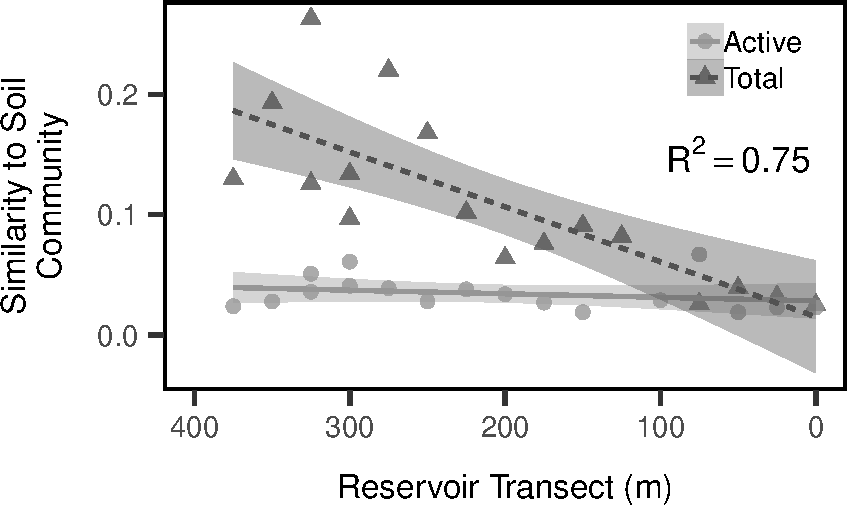
\includegraphics[width=0.7\linewidth]{ReservoirGradient_files/figure-latex/plot_similarity_to_soils-1} \end{center}

\subsection{\texorpdfstring{What about within-lake
\(\beta\)-diversity?}{What about within-lake \textbackslash{}beta-diversity?}}\label{what-about-within-lake-beta-diversity}

An alternative reason for convergence of aquatic communities along the
reservoir and decay in similarity to soils is that niche selection is
acting on aquatic community structure and driving shifts in composition
along the gradient. To test this idea, we look at the similarity of the
active and total communities to the samples taken at the dam of the
reservoir, which we expect to have a low influence of soil taxa.

\begin{Shaded}
\begin{Highlighting}[]
\CommentTok{# Similarity to Lake Samples 1 and 2}
\NormalTok{UL.bray2      <-}\StringTok{ }\DecValTok{1} \OperatorTok{-}\StringTok{ }\KeywordTok{as.matrix}\NormalTok{(}\KeywordTok{vegdist}\NormalTok{(OTUsREL.log, }\DataTypeTok{method=}\StringTok{"bray"}\NormalTok{))}
\NormalTok{UL.bray.lake2 <-}\StringTok{ }\NormalTok{UL.bray[}\OperatorTok{-}\KeywordTok{c}\NormalTok{(}\DecValTok{1}\OperatorTok{:}\DecValTok{3}\NormalTok{), }\DecValTok{4}\OperatorTok{:}\DecValTok{7}\NormalTok{]}
\NormalTok{UL.sim2       <-}\StringTok{ }\KeywordTok{cbind}\NormalTok{(design[}\OperatorTok{-}\KeywordTok{c}\NormalTok{(}\DecValTok{1}\OperatorTok{:}\DecValTok{3}\NormalTok{), ], }
                       \StringTok{"DNA"}\NormalTok{ =}\StringTok{ }\KeywordTok{apply}\NormalTok{(UL.bray.lake2[,}\KeywordTok{c}\NormalTok{(}\DecValTok{1}\NormalTok{,}\DecValTok{3}\NormalTok{)], }\DecValTok{1}\NormalTok{, mean), }
                       \StringTok{"RNA"}\NormalTok{ =}\StringTok{ }\KeywordTok{apply}\NormalTok{(UL.bray.lake2[,}\KeywordTok{c}\NormalTok{(}\DecValTok{2}\NormalTok{,}\DecValTok{4}\NormalTok{)], }\DecValTok{1}\NormalTok{, mean))}

\NormalTok{UL.sim2 }\OperatorTok\StringTok{ }\KeywordTok{gather}\NormalTok{(DNA, RNA, }\DataTypeTok{key =} \StringTok{"comparison"}\NormalTok{, }\DataTypeTok{value =} \StringTok{"similarity"}\NormalTok{) }\OperatorTok\StringTok{ }
\StringTok{  }\KeywordTok{mutate}\NormalTok{(}\DataTypeTok{molecule =} \KeywordTok{ifelse}\NormalTok{(molecule }\OperatorTok{==}\StringTok{ "DNA"}\NormalTok{, }\StringTok{"Total"}\NormalTok{, }\StringTok{"Active"}\NormalTok{),}
         \DataTypeTok{comparison =} \KeywordTok{ifelse}\NormalTok{(comparison }\OperatorTok{==}\StringTok{ "DNA"}\NormalTok{, }\StringTok{"Total"}\NormalTok{, }\StringTok{"Active"}\NormalTok{)) }\OperatorTok\StringTok{ }
\StringTok{  }\KeywordTok{ggplot}\NormalTok{(}\KeywordTok{aes}\NormalTok{(}\DataTypeTok{x =}\NormalTok{ distance, }\DataTypeTok{y =}\NormalTok{ similarity, }\DataTypeTok{color =}\NormalTok{ molecule, }\DataTypeTok{fill =}\NormalTok{ molecule)) }\OperatorTok{+}
\StringTok{  }\KeywordTok{geom_point}\NormalTok{() }\OperatorTok{+}\StringTok{ }
\StringTok{  }\KeywordTok{geom_smooth}\NormalTok{(}\DataTypeTok{method =} \StringTok{"lm"}\NormalTok{) }\OperatorTok{+}\StringTok{ }
\StringTok{  }\KeywordTok{labs}\NormalTok{(}\DataTypeTok{y =} \StringTok{"Similarity to lake community"}\NormalTok{, }
       \DataTypeTok{x =} \StringTok{"Reservoir Transect (m)"}\NormalTok{) }\OperatorTok{+}
\StringTok{  }\KeywordTok{scale_x_reverse}\NormalTok{() }\OperatorTok{+}
\StringTok{  }\KeywordTok{scale_color_manual}\NormalTok{(}\StringTok{"Community Subset"}\NormalTok{, }\DataTypeTok{values =}\NormalTok{ my.cols) }\OperatorTok{+}
\StringTok{  }\KeywordTok{scale_fill_manual}\NormalTok{(}\StringTok{"Community Subset"}\NormalTok{, }\DataTypeTok{values =}\NormalTok{ my.cols) }\OperatorTok{+}\StringTok{ }
\StringTok{  }\KeywordTok{facet_wrap}\NormalTok{(}\OperatorTok{~}\StringTok{ }\NormalTok{comparison)}
\end{Highlighting}
\end{Shaded}

\begin{center}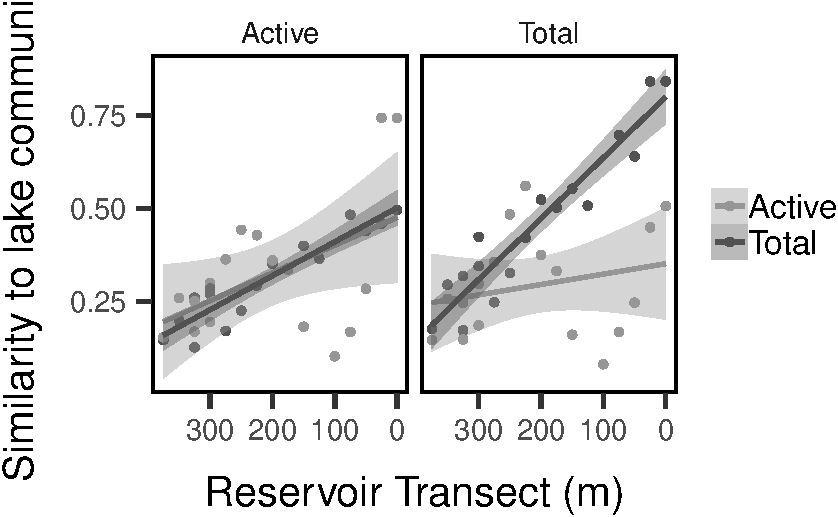
\includegraphics[width=0.7\linewidth]{ReservoirGradient_files/figure-latex/plot_similarity_to_lake-1} \end{center}

\begin{Shaded}
\begin{Highlighting}[]
\CommentTok{# Calculate Linear Model}
\NormalTok{model.lake1 <-}\StringTok{ }\KeywordTok{lm}\NormalTok{(UL.sim2}\OperatorTok{$}\NormalTok{DNA }\OperatorTok{~}\StringTok{ }\NormalTok{UL.sim2}\OperatorTok{$}\NormalTok{distance }\OperatorTok{*}\StringTok{ }\NormalTok{UL.sim2}\OperatorTok{$}\NormalTok{molecule)}
\NormalTok{model.lake2 <-}\StringTok{ }\KeywordTok{lm}\NormalTok{(UL.sim2}\OperatorTok{$}\NormalTok{RNA }\OperatorTok{~}\StringTok{ }\NormalTok{UL.sim2}\OperatorTok{$}\NormalTok{distance }\OperatorTok{*}\StringTok{ }\NormalTok{UL.sim2}\OperatorTok{$}\NormalTok{molecule)}
\KeywordTok{summary}\NormalTok{(model.lake1)}
\end{Highlighting}
\end{Shaded}

\begin{verbatim}
## 
## Call:
## lm(formula = UL.sim2$DNA ~ UL.sim2$distance * UL.sim2$molecule)
## 
## Residuals:
##       Min        1Q    Median        3Q       Max 
## -0.242239 -0.086327  0.000567  0.063327  0.271642 
## 
## Coefficients:
##                                        Estimate Std. Error t value
## (Intercept)                           0.7994111  0.0558603  14.311
## UL.sim2$distance                     -0.0016356  0.0002350  -6.960
## UL.sim2$moleculeRNA                  -0.4484387  0.0784869  -5.714
## UL.sim2$distance:UL.sim2$moleculeRNA  0.0013571  0.0003307   4.104
##                                      Pr(>|t|)    
## (Intercept)                          6.08e-15 ***
## UL.sim2$distance                     9.88e-08 ***
## UL.sim2$moleculeRNA                  3.11e-06 ***
## UL.sim2$distance:UL.sim2$moleculeRNA 0.000286 ***
## ---
## Signif. codes:  0 '***' 0.001 '**' 0.01 '*' 0.05 '.' 0.1 ' ' 1
## 
## Residual standard error: 0.1126 on 30 degrees of freedom
## Multiple R-squared:  0.6954, Adjusted R-squared:  0.6649 
## F-statistic: 22.83 on 3 and 30 DF,  p-value: 6.829e-08
\end{verbatim}

\begin{Shaded}
\begin{Highlighting}[]
\KeywordTok{summary}\NormalTok{(model.lake2)}
\end{Highlighting}
\end{Shaded}

\begin{verbatim}
## 
## Call:
## lm(formula = UL.sim2$RNA ~ UL.sim2$distance * UL.sim2$molecule)
## 
## Residuals:
##       Min        1Q    Median        3Q       Max 
## -0.298879 -0.046626 -0.003357  0.046799  0.286274 
## 
## Coefficients:
##                                        Estimate Std. Error t value
## (Intercept)                           0.5013467  0.0610169   8.217
## UL.sim2$distance                     -0.0009140  0.0002567  -3.561
## UL.sim2$moleculeRNA                  -0.0259821  0.0857323  -0.303
## UL.sim2$distance:UL.sim2$moleculeRNA  0.0001688  0.0003612   0.467
##                                      Pr(>|t|)    
## (Intercept)                          3.59e-09 ***
## UL.sim2$distance                      0.00126 ** 
## UL.sim2$moleculeRNA                   0.76393    
## UL.sim2$distance:UL.sim2$moleculeRNA  0.64353    
## ---
## Signif. codes:  0 '***' 0.001 '**' 0.01 '*' 0.05 '.' 0.1 ' ' 1
## 
## Residual standard error: 0.123 on 30 degrees of freedom
## Multiple R-squared:  0.4156, Adjusted R-squared:  0.3572 
## F-statistic: 7.112 on 3 and 30 DF,  p-value: 0.0009525
\end{verbatim}

\begin{Shaded}
\begin{Highlighting}[]
\CommentTok{# # Calculate Confidance Intervals of Model}
\CommentTok{# newdata.lake <- data.frame(cbind(UL.sim2$molecule, UL.sim2$distance))}
\CommentTok{# conf95.lake <- predict(model.lake1, newdata.lake, interval="confidence")}
\CommentTok{# }
\CommentTok{# # Dummy Variables Regression Model ("Lake Influence")}
\CommentTok{# D3 <- (UL.sim2$molecule == "RNA")*1}
\CommentTok{# fit.Fig.3c <- lm(UL.sim2$DNA ~ UL.sim2$distance + D3 + UL.sim2$distance*D3)}
\CommentTok{# # summary(fit.Fig.3c)}
\CommentTok{# }
\CommentTok{# DNA.int.3c <- fit.Fig.3c$coefficients[1]}
\CommentTok{# DNA.slp.3c <- fit.Fig.3c$coefficients[2]}
\CommentTok{# RNA.int.3c <- DNA.int.3c + fit.Fig.3c$coefficients[3]}
\CommentTok{# RNA.slp.3c <- DNA.slp.3c + fit.Fig.3c$coefficients[4]}
\end{Highlighting}
\end{Shaded}

\section{Identifying the Soil
Bacteria}\label{identifying-the-soil-bacteria}

\begin{Shaded}
\begin{Highlighting}[]
\NormalTok{soil.only <-}\StringTok{ }\NormalTok{OTUs[, }\KeywordTok{which}\NormalTok{(}\KeywordTok{colSums}\NormalTok{(OTUs[}\OperatorTok{-}\KeywordTok{c}\NormalTok{(}\DecValTok{1}\OperatorTok{:}\DecValTok{3}\NormalTok{),]) }\OperatorTok{==}\StringTok{ }\DecValTok{0}\NormalTok{)] }\CommentTok{# what is present only in soil}
\NormalTok{lake.n.soil <-}\StringTok{ }\NormalTok{OTUs[, }\KeywordTok{setdiff}\NormalTok{(}\KeywordTok{colnames}\NormalTok{(OTUs),}\KeywordTok{colnames}\NormalTok{(soil.only))] }\CommentTok{# what is present across all samples, but not just in soils}


\CommentTok{# separate lake and soil samples}
\NormalTok{lake.total <-}\StringTok{ }\NormalTok{OTUs[}\KeywordTok{which}\NormalTok{(design}\OperatorTok{$}\NormalTok{molecule }\OperatorTok{==}\StringTok{ "DNA"}\NormalTok{, design}\OperatorTok{$}\NormalTok{type }\OperatorTok{==}\StringTok{ "water"}\NormalTok{),]}
\NormalTok{soil.total <-}\StringTok{ }\NormalTok{OTUs[}\KeywordTok{which}\NormalTok{(design}\OperatorTok{$}\NormalTok{molecule }\OperatorTok{==}\StringTok{ "DNA"}\NormalTok{, design}\OperatorTok{$}\NormalTok{type }\OperatorTok{==}\StringTok{ "soil"}\NormalTok{),]}

\CommentTok{# which otus are present in both lake and soil samples}
\NormalTok{lake.and.soil.total <-}\StringTok{ }\NormalTok{OTUs[}\KeywordTok{which}\NormalTok{(design}\OperatorTok{$}\NormalTok{molecule }\OperatorTok{==}\StringTok{ "DNA"}\NormalTok{, design}\OperatorTok{$}\NormalTok{type }\OperatorTok{==}\StringTok{ "water"}\NormalTok{),}
                            \KeywordTok{which}\NormalTok{(}\KeywordTok{colSums}\NormalTok{(lake.total) }\OperatorTok{>}\StringTok{ }\DecValTok{0} \OperatorTok{&}\StringTok{ }\KeywordTok{colSums}\NormalTok{(soil.total) }\OperatorTok{>}\StringTok{ }\DecValTok{0}\NormalTok{)]}

\CommentTok{# isolate just the dna and rna lake communities}
\NormalTok{w.dna <-}\StringTok{ }\NormalTok{OTUs[}\KeywordTok{which}\NormalTok{(design}\OperatorTok{$}\NormalTok{molecule }\OperatorTok{==}\StringTok{ "DNA"} \OperatorTok{&}\StringTok{ }\NormalTok{design}\OperatorTok{$}\NormalTok{type }\OperatorTok{==}\StringTok{ "water"}\NormalTok{), ]}
\NormalTok{w.rna <-}\StringTok{ }\NormalTok{OTUs[}\KeywordTok{which}\NormalTok{(design}\OperatorTok{$}\NormalTok{molecule }\OperatorTok{==}\StringTok{ "RNA"} \OperatorTok{&}\StringTok{ }\NormalTok{design}\OperatorTok{$}\NormalTok{type }\OperatorTok{==}\StringTok{ "water"}\NormalTok{), ]}

\CommentTok{# pull out the lake rna counds for otus found in lake and soil}
\NormalTok{lake.and.soil.act <-}\StringTok{ }\NormalTok{w.rna[,}\KeywordTok{colnames}\NormalTok{(lake.and.soil.total)]}

\CommentTok{# of these lake and soil taxa, which are never active?}
\NormalTok{nvr.act <-}\StringTok{ }\KeywordTok{which}\NormalTok{(}\KeywordTok{colSums}\NormalTok{(lake.and.soil.act) }\OperatorTok{==}\StringTok{ }\DecValTok{0}\NormalTok{)}

\CommentTok{# pull out their dna abundances and calculate richness}
\NormalTok{terr.lake <-}\StringTok{ }\NormalTok{w.dna[ , }\KeywordTok{c}\NormalTok{(}\KeywordTok{names}\NormalTok{(nvr.act))]}
\NormalTok{terr.rich <-}\StringTok{ }\KeywordTok{rowSums}\NormalTok{((terr.lake }\OperatorTok{>}\StringTok{ }\DecValTok{0}\NormalTok{) }\OperatorTok{*}\StringTok{ }\DecValTok{1}\NormalTok{)}
\NormalTok{terr.REL <-}\StringTok{ }\KeywordTok{rowSums}\NormalTok{(terr.lake) }\OperatorTok{/}\StringTok{ }\KeywordTok{rowSums}\NormalTok{(w.dna) }
\NormalTok{design.dna <-}\StringTok{ }\NormalTok{design[}\KeywordTok{which}\NormalTok{(design}\OperatorTok{$}\NormalTok{molecule }\OperatorTok{==}\StringTok{ "DNA"} \OperatorTok{&}\StringTok{ }\NormalTok{design}\OperatorTok{$}\NormalTok{type }\OperatorTok{==}\StringTok{ "water"}\NormalTok{), ]}
\NormalTok{terr.rich.log <-}\StringTok{ }\KeywordTok{log10}\NormalTok{(terr.rich)}
\NormalTok{terr.REL.log <-}\StringTok{ }\KeywordTok{log10}\NormalTok{(terr.REL)}

\NormalTok{terr.mod1 <-}\StringTok{ }\KeywordTok{lm}\NormalTok{(terr.rich.log }\OperatorTok{~}\StringTok{ }\NormalTok{design.dna}\OperatorTok{$}\NormalTok{distance)}
\KeywordTok{summary}\NormalTok{(terr.mod1)}
\end{Highlighting}
\end{Shaded}

\begin{verbatim}
## 
## Call:
## lm(formula = terr.rich.log ~ design.dna$distance)
## 
## Residuals:
##      Min       1Q   Median       3Q      Max 
## -0.23774 -0.13355  0.05749  0.10655  0.22647 
## 
## Coefficients:
##                      Estimate Std. Error t value Pr(>|t|)    
## (Intercept)         2.0158897  0.0771478   26.13 6.36e-14 ***
## design.dna$distance 0.0031610  0.0003245    9.74 7.06e-08 ***
## ---
## Signif. codes:  0 '***' 0.001 '**' 0.01 '*' 0.05 '.' 0.1 ' ' 1
## 
## Residual standard error: 0.1555 on 15 degrees of freedom
## Multiple R-squared:  0.8635, Adjusted R-squared:  0.8544 
## F-statistic: 94.87 on 1 and 15 DF,  p-value: 7.059e-08
\end{verbatim}

\begin{Shaded}
\begin{Highlighting}[]
\NormalTok{T1.R2 <-}\StringTok{ }\KeywordTok{round}\NormalTok{(}\KeywordTok{summary}\NormalTok{(terr.mod1)}\OperatorTok{$}\NormalTok{r.squared, }\DecValTok{2}\NormalTok{)}
\NormalTok{T1.int <-}\StringTok{ }\NormalTok{terr.mod1}\OperatorTok{$}\NormalTok{coefficients[}\DecValTok{1}\NormalTok{]}
\NormalTok{T1.slp <-}\StringTok{ }\NormalTok{terr.mod1}\OperatorTok{$}\NormalTok{coefficients[}\DecValTok{2}\NormalTok{]}
\KeywordTok{pander}\NormalTok{(terr.mod1)}
\end{Highlighting}
\end{Shaded}

\begin{longtable}[]{@{}ccccc@{}}
\caption{Fitting linear model: terr.rich.log \textasciitilde{}
design.dna\$distance}\tabularnewline
\toprule
\begin{minipage}[b]{0.31\columnwidth}\centering\strut
~\strut
\end{minipage} & \begin{minipage}[b]{0.13\columnwidth}\centering\strut
Estimate\strut
\end{minipage} & \begin{minipage}[b]{0.16\columnwidth}\centering\strut
Std. Error\strut
\end{minipage} & \begin{minipage}[b]{0.12\columnwidth}\centering\strut
t value\strut
\end{minipage} & \begin{minipage}[b]{0.13\columnwidth}\centering\strut
Pr(\textgreater{}\textbar{}t\textbar{})\strut
\end{minipage}\tabularnewline
\midrule
\endfirsthead
\toprule
\begin{minipage}[b]{0.31\columnwidth}\centering\strut
~\strut
\end{minipage} & \begin{minipage}[b]{0.13\columnwidth}\centering\strut
Estimate\strut
\end{minipage} & \begin{minipage}[b]{0.16\columnwidth}\centering\strut
Std. Error\strut
\end{minipage} & \begin{minipage}[b]{0.12\columnwidth}\centering\strut
t value\strut
\end{minipage} & \begin{minipage}[b]{0.13\columnwidth}\centering\strut
Pr(\textgreater{}\textbar{}t\textbar{})\strut
\end{minipage}\tabularnewline
\midrule
\endhead
\begin{minipage}[t]{0.31\columnwidth}\centering\strut
\textbf{(Intercept)}\strut
\end{minipage} & \begin{minipage}[t]{0.13\columnwidth}\centering\strut
2.016\strut
\end{minipage} & \begin{minipage}[t]{0.16\columnwidth}\centering\strut
0.07715\strut
\end{minipage} & \begin{minipage}[t]{0.12\columnwidth}\centering\strut
26.13\strut
\end{minipage} & \begin{minipage}[t]{0.13\columnwidth}\centering\strut
6.362e-14\strut
\end{minipage}\tabularnewline
\begin{minipage}[t]{0.31\columnwidth}\centering\strut
\textbf{design.dna\$distance}\strut
\end{minipage} & \begin{minipage}[t]{0.13\columnwidth}\centering\strut
0.003161\strut
\end{minipage} & \begin{minipage}[t]{0.16\columnwidth}\centering\strut
0.0003245\strut
\end{minipage} & \begin{minipage}[t]{0.12\columnwidth}\centering\strut
9.74\strut
\end{minipage} & \begin{minipage}[t]{0.13\columnwidth}\centering\strut
7.059e-08\strut
\end{minipage}\tabularnewline
\bottomrule
\end{longtable}

\begin{Shaded}
\begin{Highlighting}[]
\CommentTok{# terr.mod2 <- lm(terr.REL.log ~ design.dna$distance)}
\CommentTok{# summary(terr.mod2)}
\CommentTok{# T2.R2 <- round(summary(terr.mod2)$r.squared, 2)}
\CommentTok{# T2.int <- terr.mod2$coefficients[1]}
\CommentTok{# T2.slp <- terr.mod2$coefficients[2]}
\end{Highlighting}
\end{Shaded}

\subsection{Figure 4: Transient decay}\label{figure-4-transient-decay}

\begin{Shaded}
\begin{Highlighting}[]
\KeywordTok{tibble}\NormalTok{(}\DataTypeTok{transient_rich =}\NormalTok{ terr.rich, }\DataTypeTok{distance =}\NormalTok{ design.dna}\OperatorTok{$}\NormalTok{distance) }\OperatorTok\StringTok{ }
\StringTok{  }\KeywordTok{ggplot}\NormalTok{(}\KeywordTok{aes}\NormalTok{(}\DataTypeTok{x =}\NormalTok{ distance, }\DataTypeTok{y =}\NormalTok{ transient_rich)) }\OperatorTok{+}\StringTok{ }
\StringTok{  }\KeywordTok{geom_smooth}\NormalTok{(}\DataTypeTok{method =} \StringTok{"lm"}\NormalTok{, }\DataTypeTok{color =} \StringTok{"black"}\NormalTok{, }\DataTypeTok{fill =} \StringTok{"grey"}\NormalTok{) }\OperatorTok{+}
\StringTok{  }\KeywordTok{geom_point}\NormalTok{(}\DataTypeTok{alpha =} \DecValTok{1}\NormalTok{, }\DataTypeTok{color =} \StringTok{"black"}\NormalTok{) }\OperatorTok{+}\StringTok{ }
\StringTok{  }\KeywordTok{scale_x_reverse}\NormalTok{(}\DataTypeTok{limits =} \KeywordTok{c}\NormalTok{(}\DecValTok{400}\NormalTok{,}\DecValTok{0}\NormalTok{)) }\OperatorTok{+}
\StringTok{  }\KeywordTok{scale_y_log10}\NormalTok{() }\OperatorTok{+}
\StringTok{  }\KeywordTok{annotation_logticks}\NormalTok{(}\DataTypeTok{sides =} \StringTok{"l"}\NormalTok{) }\OperatorTok{+}
\StringTok{  }\KeywordTok{labs}\NormalTok{(}\DataTypeTok{x =} \StringTok{"Reservoir Transect (m)"}\NormalTok{,}
       \DataTypeTok{y =} \StringTok{"Soil-derived Taxa Richness"}\NormalTok{) }\OperatorTok{+}
\StringTok{  }\KeywordTok{annotate}\NormalTok{(}\StringTok{"text"}\NormalTok{, }\DataTypeTok{x =} \DecValTok{50}\NormalTok{, }\DataTypeTok{y =} \DecValTok{750}\NormalTok{, }\DataTypeTok{size =} \DecValTok{6}\NormalTok{, }\DataTypeTok{label =} \KeywordTok{paste0}\NormalTok{(}\StringTok{"R^2== "}\NormalTok{,T1.R2), }\DataTypeTok{parse =}\NormalTok{ T) }
\end{Highlighting}
\end{Shaded}

\begin{center}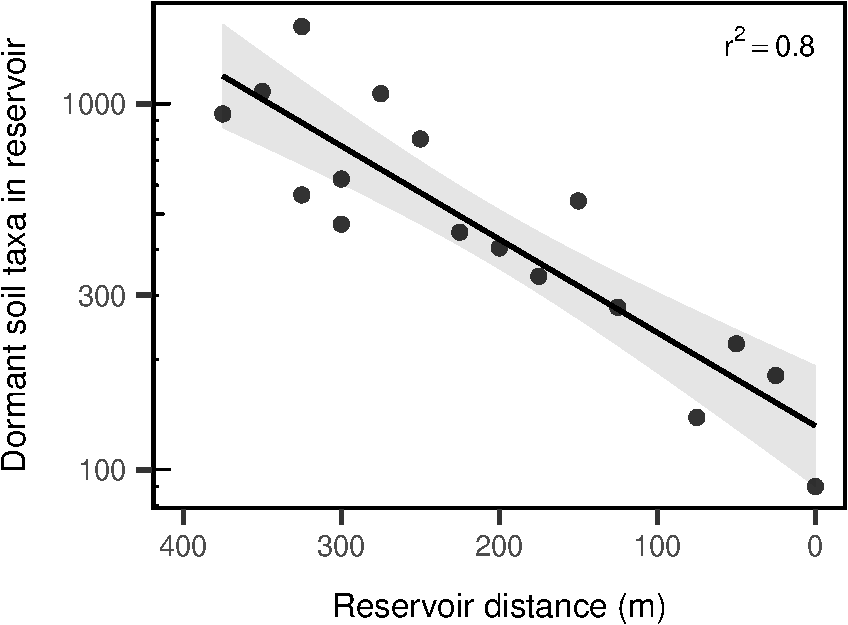
\includegraphics[width=0.7\linewidth]{ReservoirGradient_files/figure-latex/plot_transient-1} \end{center}

\section{Define Core Lake Taxa}\label{define-core-lake-taxa}

\begin{Shaded}
\begin{Highlighting}[]
\CommentTok{# identify otus in soil samples and lake samples}
\NormalTok{in.soil <-}\StringTok{ }\NormalTok{OTUs[, }\KeywordTok{which}\NormalTok{(}\KeywordTok{colSums}\NormalTok{(OTUs[}\KeywordTok{c}\NormalTok{(}\DecValTok{1}\OperatorTok{:}\DecValTok{3}\NormalTok{),]) }\OperatorTok{>}\StringTok{ }\DecValTok{0}\NormalTok{ )]}
\NormalTok{in.lake <-}\StringTok{ }\NormalTok{OTUs[, }\KeywordTok{which}\NormalTok{(}\KeywordTok{colSums}\NormalTok{(OTUs[}\OperatorTok{-}\KeywordTok{c}\NormalTok{(}\DecValTok{1}\OperatorTok{:}\DecValTok{3}\NormalTok{),]) }\OperatorTok{>}\StringTok{ }\DecValTok{0}\NormalTok{)]}

\CommentTok{# isolate just the rna water samples and convert to presence-absence}
\NormalTok{in.lake.rna <-}\StringTok{ }\NormalTok{in.lake[}\KeywordTok{which}\NormalTok{(design}\OperatorTok{$}\NormalTok{molecule }\OperatorTok{==}\StringTok{ "RNA"} \OperatorTok{&}\StringTok{ }\NormalTok{design}\OperatorTok{$}\NormalTok{type }\OperatorTok{==}\StringTok{ "water"}\NormalTok{), ]}
\NormalTok{in.lake.rna.pa <-}\StringTok{ }\NormalTok{(in.lake.rna }\OperatorTok{>}\StringTok{ }\DecValTok{0}\NormalTok{) }\OperatorTok{*}\StringTok{ }\DecValTok{1}

\CommentTok{# define the 'core' taxa as otus present in 90% of samples}
\NormalTok{in.lake.core <-}\StringTok{ }\NormalTok{w.dna[, }\KeywordTok{which}\NormalTok{((}\KeywordTok{colSums}\NormalTok{(in.lake.rna.pa) }\OperatorTok{/}\StringTok{ }\KeywordTok{nrow}\NormalTok{(in.lake.rna.pa)) }\OperatorTok{>=}\StringTok{ }\FloatTok{0.8}\NormalTok{)]}

\CommentTok{# of the core, how many are also in the soil samples?}
\NormalTok{in.lake.core.from.soils <-}\StringTok{ }\NormalTok{in.lake.core[, }\KeywordTok{intersect}\NormalTok{(}\KeywordTok{colnames}\NormalTok{(in.lake.core), }\KeywordTok{colnames}\NormalTok{(in.soil))]}

\CommentTok{# of the core which are not in the soil samples}
\NormalTok{in.lake.core.not.soils <-}\StringTok{ }\NormalTok{in.lake.core[, }\KeywordTok{setdiff}\NormalTok{(}\KeywordTok{colnames}\NormalTok{(in.lake.core), }\KeywordTok{colnames}\NormalTok{(in.soil))]}


\NormalTok{in.lake.core.from.soils.REL <-}\StringTok{ }\NormalTok{in.lake.core.from.soils }\OperatorTok{/}\StringTok{ }\KeywordTok{rowSums}\NormalTok{(w.dna)}

\NormalTok{in.soil.to.plot <-}\StringTok{ }\KeywordTok{as.data.frame}\NormalTok{(in.lake.core.from.soils.REL) }\OperatorTok\StringTok{ }
\StringTok{  }\KeywordTok{rownames_to_column}\NormalTok{(}\StringTok{"sample_ID"}\NormalTok{) }\OperatorTok\StringTok{ }
\StringTok{  }\KeywordTok{gather}\NormalTok{(otu_id, rel_abundance, }\OperatorTok{-}\NormalTok{sample_ID) }\OperatorTok\StringTok{ }
\StringTok{  }\KeywordTok{left_join}\NormalTok{(}\KeywordTok{rownames_to_column}\NormalTok{(design.dna, }\StringTok{"sample_ID"}\NormalTok{)) }\OperatorTok\StringTok{ }
\StringTok{  }\KeywordTok{add_column}\NormalTok{(}\DataTypeTok{found =} \StringTok{"soils"}\NormalTok{)}

\NormalTok{in.lake.core.not.soils.REL <-}\StringTok{ }\NormalTok{in.lake.core.not.soils }\OperatorTok{/}\StringTok{ }\KeywordTok{rowSums}\NormalTok{(w.dna)}

\NormalTok{in.lake.to.plot <-}\StringTok{ }\KeywordTok{as.data.frame}\NormalTok{(in.lake.core.not.soils.REL) }\OperatorTok\StringTok{ }
\StringTok{  }\KeywordTok{rownames_to_column}\NormalTok{(}\StringTok{"sample_ID"}\NormalTok{) }\OperatorTok\StringTok{ }
\StringTok{  }\KeywordTok{gather}\NormalTok{(otu_id, rel_abundance, }\OperatorTok{-}\NormalTok{sample_ID) }\OperatorTok\StringTok{ }
\StringTok{  }\KeywordTok{left_join}\NormalTok{(}\KeywordTok{rownames_to_column}\NormalTok{(design.dna, }\StringTok{"sample_ID"}\NormalTok{)) }\OperatorTok\StringTok{ }
\StringTok{  }\KeywordTok{add_column}\NormalTok{(}\DataTypeTok{found =} \StringTok{"lake"}\NormalTok{)}
\end{Highlighting}
\end{Shaded}

Now, lets plot the abundances of the OTUs across the reservoir and split
them up into whether they were recovered in soils or not.

\begin{Shaded}
\begin{Highlighting}[]
\KeywordTok{bind_rows}\NormalTok{(in.soil.to.plot, in.lake.to.plot) }\OperatorTok\StringTok{ }
\StringTok{  }\KeywordTok{ggplot}\NormalTok{(}\KeywordTok{aes}\NormalTok{(}\DataTypeTok{x =}\NormalTok{ distance, }\DataTypeTok{y =}\NormalTok{ rel_abundance, }\DataTypeTok{color =}\NormalTok{ otu_id)) }\OperatorTok{+}\StringTok{ }
\StringTok{  }\KeywordTok{labs}\NormalTok{(}\DataTypeTok{x =} \StringTok{"Reservoir Transect (m)"}\NormalTok{, }
       \DataTypeTok{y =} \StringTok{"OTU Relative Abundance"}\NormalTok{) }\OperatorTok{+}
\StringTok{  }\KeywordTok{geom_line}\NormalTok{(}\DataTypeTok{alpha =} \FloatTok{0.25}\NormalTok{, }\DataTypeTok{stat =} \StringTok{"smooth"}\NormalTok{, }\DataTypeTok{method =} \StringTok{"lm"}\NormalTok{, }\DataTypeTok{se =}\NormalTok{ F, }\DataTypeTok{show.legend =}\NormalTok{ F) }\OperatorTok{+}
\StringTok{  }\KeywordTok{facet_wrap}\NormalTok{(}\OperatorTok{~}\StringTok{ }\NormalTok{found, }\DataTypeTok{ncol =} \DecValTok{1}\NormalTok{)}
\end{Highlighting}
\end{Shaded}

\begin{center}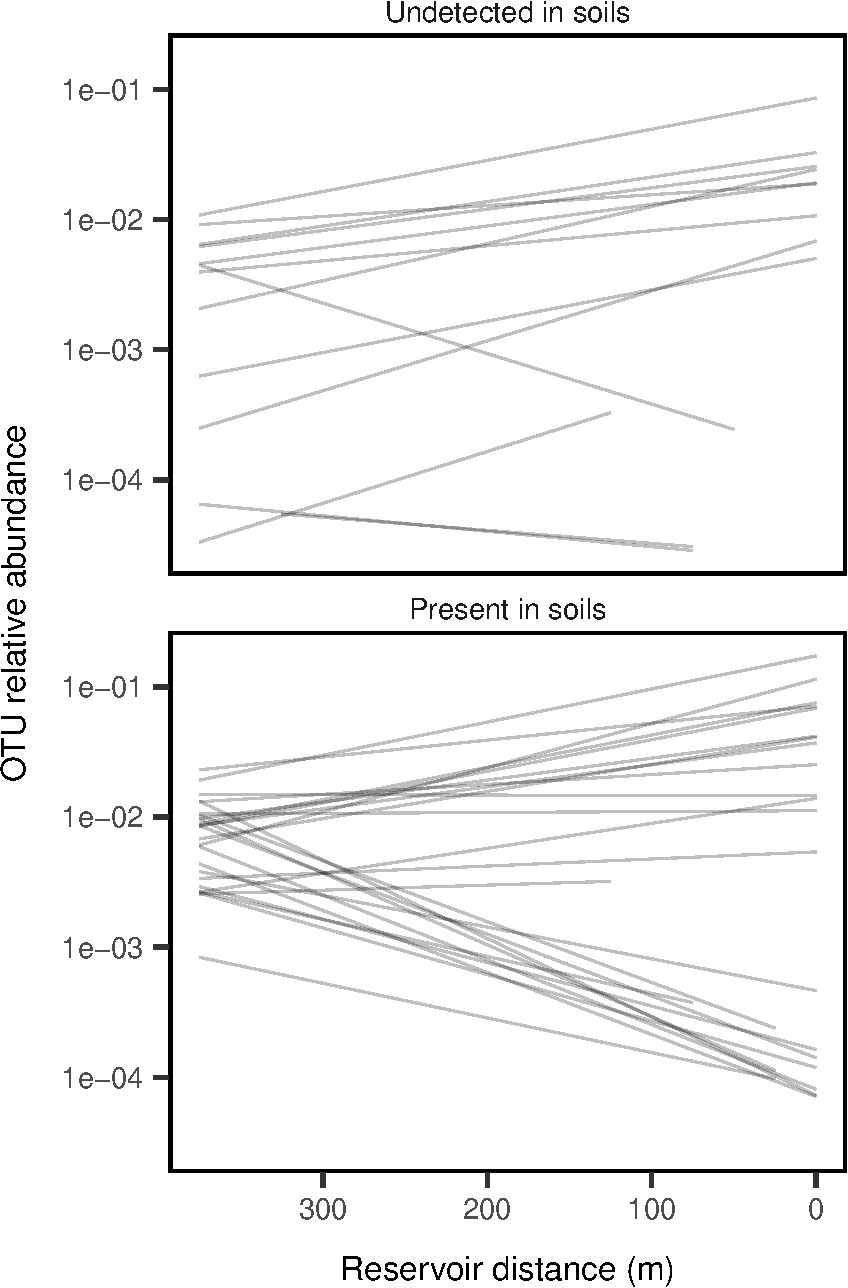
\includegraphics[width=0.7\linewidth]{ReservoirGradient_files/figure-latex/coreplot-1} \end{center}

\begin{Shaded}
\begin{Highlighting}[]
\KeywordTok{data.frame}\NormalTok{(}\DataTypeTok{mean_relabund =} \KeywordTok{colMeans}\NormalTok{(in.lake.core.from.soils.REL)) }\OperatorTok\StringTok{ }
\StringTok{  }\KeywordTok{rownames_to_column}\NormalTok{(}\DataTypeTok{var =} \StringTok{"OTU"}\NormalTok{) }\OperatorTok\StringTok{ }\KeywordTok{left_join}\NormalTok{(OTU.tax) }\OperatorTok\StringTok{ }
\StringTok{  }\KeywordTok{mutate}\NormalTok{(}\DataTypeTok{Taxon =} \KeywordTok{paste}\NormalTok{(Phylum, Class, Order)) }\OperatorTok\StringTok{ }
\StringTok{  }\KeywordTok{arrange}\NormalTok{(}\KeywordTok{desc}\NormalTok{(mean_relabund)) }\OperatorTok\StringTok{ }
\StringTok{  }\KeywordTok{ggplot}\NormalTok{() }\OperatorTok{+}\StringTok{ }
\StringTok{  }\KeywordTok{geom_bar}\NormalTok{(}\KeywordTok{aes}\NormalTok{(}\DataTypeTok{x =}\NormalTok{ Taxon, }\DataTypeTok{y =}\NormalTok{ mean_relabund), }\DataTypeTok{stat =} \StringTok{"identity"}\NormalTok{) }\OperatorTok{+}
\StringTok{  }\KeywordTok{coord_flip}\NormalTok{()}
\end{Highlighting}
\end{Shaded}

\begin{verbatim}
## Warning: Column `OTU` joining character vector and factor, coercing into
## character vector
\end{verbatim}

\begin{center}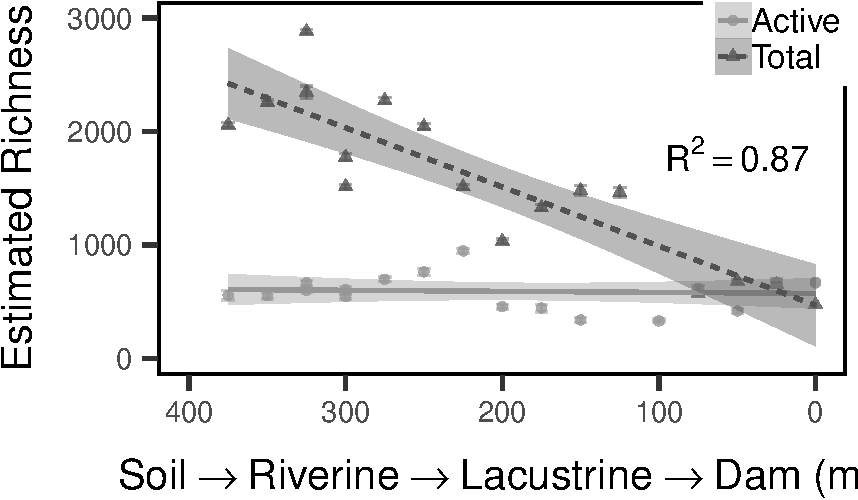
\includegraphics[width=0.7\linewidth]{ReservoirGradient_files/figure-latex/unnamed-chunk-4-1} \end{center}

\begin{Shaded}
\begin{Highlighting}[]
\NormalTok{soil.core.mods <-}\StringTok{ }\KeywordTok{apply}\NormalTok{(in.lake.core.from.soils.REL, }\DataTypeTok{MARGIN =} \DecValTok{2}\NormalTok{, }
    \DataTypeTok{FUN =} \ControlFlowTok{function}\NormalTok{(x) }\KeywordTok{summary}\NormalTok{(}\KeywordTok{lm}\NormalTok{(x }\OperatorTok{~}\StringTok{ }\NormalTok{design.dna}\OperatorTok{$}\NormalTok{distance))}\OperatorTok{$}\NormalTok{coefficients[}\DecValTok{2}\NormalTok{,}\KeywordTok{c}\NormalTok{(}\DecValTok{1}\NormalTok{,}\DecValTok{4}\NormalTok{)])}
\KeywordTok{rownames}\NormalTok{(soil.core.mods) <-}\StringTok{ }\KeywordTok{c}\NormalTok{(}\StringTok{"slope"}\NormalTok{, }\StringTok{"pval"}\NormalTok{)}
\NormalTok{soil.core.decresing <-}\StringTok{ }\KeywordTok{as.data.frame}\NormalTok{(}\KeywordTok{t}\NormalTok{(soil.core.mods)) }\OperatorTok\StringTok{ }
\StringTok{  }\KeywordTok{rownames_to_column}\NormalTok{(}\StringTok{"OTU"}\NormalTok{) }\OperatorTok\StringTok{ }
\StringTok{  }\KeywordTok{filter}\NormalTok{(pval }\OperatorTok{<}\StringTok{ }\FloatTok{0.05} \OperatorTok{&}\StringTok{ }\NormalTok{slope }\OperatorTok{>}\StringTok{ }\DecValTok{0}\NormalTok{) }\OperatorTok\StringTok{   }\CommentTok{# rel abund decreases toward dam}
\StringTok{  }\KeywordTok{left_join}\NormalTok{(OTU.tax)}
\end{Highlighting}
\end{Shaded}

\begin{verbatim}
## Warning: Column `OTU` joining character vector and factor, coercing into
## character vector
\end{verbatim}

\begin{Shaded}
\begin{Highlighting}[]
\NormalTok{soil.core.increasing <-}\StringTok{ }\KeywordTok{as.data.frame}\NormalTok{(}\KeywordTok{t}\NormalTok{(soil.core.mods)) }\OperatorTok\StringTok{ }
\StringTok{  }\KeywordTok{rownames_to_column}\NormalTok{(}\StringTok{"OTU"}\NormalTok{) }\OperatorTok\StringTok{ }
\StringTok{  }\KeywordTok{filter}\NormalTok{(pval }\OperatorTok{<}\StringTok{ }\FloatTok{0.05} \OperatorTok{&}\StringTok{ }\NormalTok{slope }\OperatorTok{<}\StringTok{ }\DecValTok{0}\NormalTok{) }\OperatorTok\StringTok{   }\CommentTok{# rel abund increases toward dam}
\StringTok{  }\KeywordTok{left_join}\NormalTok{(OTU.tax)}
\end{Highlighting}
\end{Shaded}

\begin{verbatim}
## Warning: Column `OTU` joining character vector and factor, coercing into
## character vector
\end{verbatim}

\begin{Shaded}
\begin{Highlighting}[]
\KeywordTok{data.frame}\NormalTok{(}\DataTypeTok{mean_relabund =} \KeywordTok{colMeans}\NormalTok{(in.lake.core.not.soils.REL)) }\OperatorTok\StringTok{ }
\StringTok{  }\KeywordTok{rownames_to_column}\NormalTok{(}\DataTypeTok{var =} \StringTok{"OTU"}\NormalTok{) }\OperatorTok\StringTok{ }\KeywordTok{left_join}\NormalTok{(OTU.tax) }\OperatorTok\StringTok{ }
\StringTok{  }\KeywordTok{mutate}\NormalTok{(}\DataTypeTok{Taxon =} \KeywordTok{paste}\NormalTok{(Phylum, Class, Order)) }\OperatorTok\StringTok{ }
\StringTok{  }\KeywordTok{arrange}\NormalTok{(}\KeywordTok{desc}\NormalTok{(mean_relabund)) }\OperatorTok\StringTok{ }
\StringTok{  }\KeywordTok{ggplot}\NormalTok{() }\OperatorTok{+}\StringTok{ }
\StringTok{  }\KeywordTok{geom_bar}\NormalTok{(}\KeywordTok{aes}\NormalTok{(}\DataTypeTok{x =}\NormalTok{ Taxon, }\DataTypeTok{y =}\NormalTok{ mean_relabund), }\DataTypeTok{stat =} \StringTok{"identity"}\NormalTok{) }\OperatorTok{+}
\StringTok{  }\KeywordTok{coord_flip}\NormalTok{()}
\end{Highlighting}
\end{Shaded}

\begin{verbatim}
## Warning: Column `OTU` joining character vector and factor, coercing into
## character vector
\end{verbatim}

\begin{center}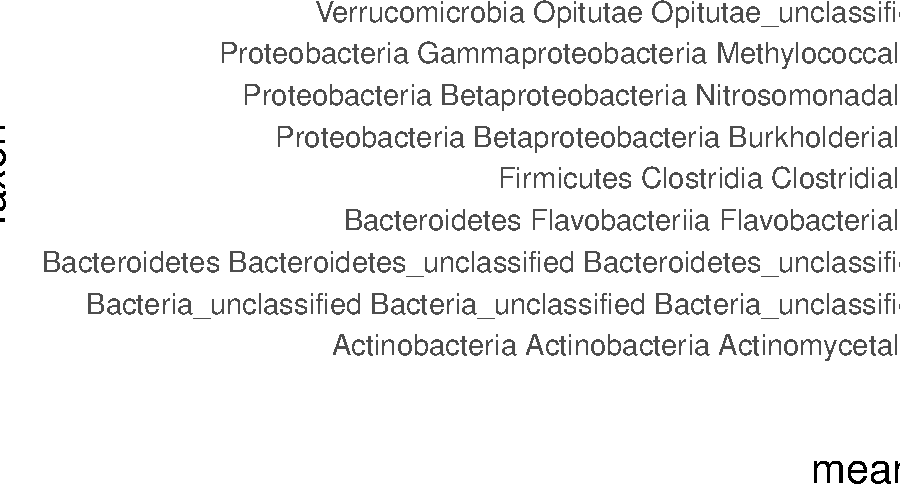
\includegraphics[width=0.7\linewidth]{ReservoirGradient_files/figure-latex/unnamed-chunk-4-2} \end{center}

\begin{Shaded}
\begin{Highlighting}[]
\NormalTok{nonsoil.core.mods <-}\StringTok{ }\KeywordTok{apply}\NormalTok{(in.lake.core.not.soils.REL, }\DataTypeTok{MARGIN =} \DecValTok{2}\NormalTok{, }\DataTypeTok{FUN =} \ControlFlowTok{function}\NormalTok{(x) }\KeywordTok{summary}\NormalTok{(}\KeywordTok{lm}\NormalTok{(x }\OperatorTok{~}\StringTok{ }\NormalTok{design.dna}\OperatorTok{$}\NormalTok{distance))}\OperatorTok{$}\NormalTok{coefficients[}\DecValTok{2}\NormalTok{,}\KeywordTok{c}\NormalTok{(}\DecValTok{1}\NormalTok{,}\DecValTok{4}\NormalTok{)])}
\KeywordTok{rownames}\NormalTok{(nonsoil.core.mods) <-}\StringTok{ }\KeywordTok{c}\NormalTok{(}\StringTok{"slope"}\NormalTok{, }\StringTok{"pval"}\NormalTok{)}
\NormalTok{nonsoil.core.decreasing <-}\StringTok{ }\KeywordTok{as.data.frame}\NormalTok{(}\KeywordTok{t}\NormalTok{(nonsoil.core.mods)) }\OperatorTok\StringTok{ }
\StringTok{  }\KeywordTok{rownames_to_column}\NormalTok{(}\StringTok{"OTU"}\NormalTok{) }\OperatorTok\StringTok{ }
\StringTok{  }\KeywordTok{filter}\NormalTok{(pval }\OperatorTok{<}\StringTok{ }\FloatTok{0.05} \OperatorTok{&}\StringTok{ }\NormalTok{slope }\OperatorTok{>}\StringTok{ }\DecValTok{0}\NormalTok{) }\OperatorTok\StringTok{   }\CommentTok{# rel abund decreases toward dam}
\StringTok{  }\KeywordTok{left_join}\NormalTok{(OTU.tax)}
\end{Highlighting}
\end{Shaded}

\begin{verbatim}
## Warning: Column `OTU` joining character vector and factor, coercing into
## character vector
\end{verbatim}

\begin{Shaded}
\begin{Highlighting}[]
\NormalTok{nonsoil.core.increasing <-}\StringTok{ }\KeywordTok{as.data.frame}\NormalTok{(}\KeywordTok{t}\NormalTok{(nonsoil.core.mods)) }\OperatorTok\StringTok{ }
\StringTok{  }\KeywordTok{rownames_to_column}\NormalTok{(}\StringTok{"OTU"}\NormalTok{) }\OperatorTok\StringTok{ }
\StringTok{  }\KeywordTok{filter}\NormalTok{(pval }\OperatorTok{<}\StringTok{ }\FloatTok{0.05} \OperatorTok{&}\StringTok{ }\NormalTok{slope }\OperatorTok{<}\StringTok{ }\DecValTok{0}\NormalTok{) }\OperatorTok\StringTok{   }\CommentTok{# rel abund increases toward dam}
\StringTok{  }\KeywordTok{left_join}\NormalTok{(OTU.tax)}
\end{Highlighting}
\end{Shaded}

\begin{verbatim}
## Warning: Column `OTU` joining character vector and factor, coercing into
## character vector
\end{verbatim}

\begin{Shaded}
\begin{Highlighting}[]
\KeywordTok{as.data.frame}\NormalTok{(OTUsREL[,nonsoil.core.increasing}\OperatorTok{$}\NormalTok{OTU]) }\OperatorTok\StringTok{ }\KeywordTok{rownames_to_column}\NormalTok{(}\StringTok{"sampleID"}\NormalTok{) }\OperatorTok\StringTok{ }
\StringTok{  }\KeywordTok{left_join}\NormalTok{(}\KeywordTok{rownames_to_column}\NormalTok{(design, }\StringTok{"sampleID"}\NormalTok{)) }\OperatorTok\StringTok{ }
\StringTok{  }\KeywordTok{gather}\NormalTok{(OTU, rel_abund, }\OperatorTok{-}\NormalTok{station, }\OperatorTok{-}\NormalTok{molecule, }\OperatorTok{-}\NormalTok{type, }\OperatorTok{-}\NormalTok{distance, }\OperatorTok{-}\NormalTok{sampleID) }\OperatorTok\StringTok{ }
\StringTok{  }\KeywordTok{filter}\NormalTok{(molecule }\OperatorTok{==}\StringTok{ "DNA"}\NormalTok{) }\OperatorTok\StringTok{ }\KeywordTok{left_join}\NormalTok{(OTU.tax) }\OperatorTok\StringTok{ }
\StringTok{  }\KeywordTok{mutate}\NormalTok{(}\DataTypeTok{taxon =} \KeywordTok{paste}\NormalTok{(Class, Order, Family)) }\OperatorTok\StringTok{ }
\StringTok{  }\KeywordTok{ggplot}\NormalTok{(}\KeywordTok{aes}\NormalTok{(}\DataTypeTok{x =}\NormalTok{ distance, }\DataTypeTok{y =}\NormalTok{ rel_abund, }\DataTypeTok{color =}\NormalTok{ taxon)) }\OperatorTok{+}\StringTok{ }
\StringTok{  }\KeywordTok{geom_point}\NormalTok{() }\OperatorTok{+}\StringTok{ }
\StringTok{  }\KeywordTok{geom_smooth}\NormalTok{(}\DataTypeTok{method =} \StringTok{"lm"}\NormalTok{) }\OperatorTok{+}\StringTok{ }
\StringTok{  }\KeywordTok{scale_x_reverse}\NormalTok{()}
\end{Highlighting}
\end{Shaded}

\begin{verbatim}
## Warning: Column `OTU` joining character vector and factor, coercing into
## character vector
\end{verbatim}

\begin{verbatim}
## Warning: Removed 15 rows containing non-finite values (stat_smooth).
\end{verbatim}

\begin{verbatim}
## Warning: Removed 15 rows containing missing values (geom_point).
\end{verbatim}

\begin{center}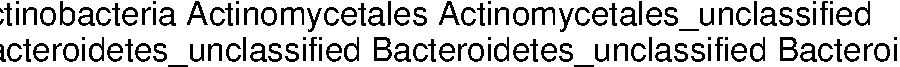
\includegraphics[width=0.7\linewidth]{ReservoirGradient_files/figure-latex/unnamed-chunk-4-3} \end{center}

\begin{Shaded}
\begin{Highlighting}[]
\KeywordTok{as.data.frame}\NormalTok{(OTUsREL[,soil.core.increasing}\OperatorTok{$}\NormalTok{OTU]) }\OperatorTok\StringTok{ }\KeywordTok{rownames_to_column}\NormalTok{(}\StringTok{"sampleID"}\NormalTok{) }\OperatorTok\StringTok{ }
\StringTok{  }\KeywordTok{left_join}\NormalTok{(}\KeywordTok{rownames_to_column}\NormalTok{(design, }\StringTok{"sampleID"}\NormalTok{)) }\OperatorTok\StringTok{ }
\StringTok{  }\KeywordTok{gather}\NormalTok{(OTU, rel_abund, }\OperatorTok{-}\NormalTok{station, }\OperatorTok{-}\NormalTok{molecule, }\OperatorTok{-}\NormalTok{type, }\OperatorTok{-}\NormalTok{distance, }\OperatorTok{-}\NormalTok{sampleID) }\OperatorTok\StringTok{ }
\StringTok{  }\KeywordTok{filter}\NormalTok{(molecule }\OperatorTok{==}\StringTok{ "DNA"}\NormalTok{) }\OperatorTok\StringTok{ }\KeywordTok{left_join}\NormalTok{(OTU.tax) }\OperatorTok\StringTok{ }
\StringTok{  }\KeywordTok{mutate}\NormalTok{(}\DataTypeTok{taxon =} \KeywordTok{paste}\NormalTok{(Class, Order, Family)) }\OperatorTok\StringTok{ }
\StringTok{  }\KeywordTok{ggplot}\NormalTok{(}\KeywordTok{aes}\NormalTok{(}\DataTypeTok{x =}\NormalTok{ distance, }\DataTypeTok{y =}\NormalTok{ rel_abund, }\DataTypeTok{color =}\NormalTok{ taxon)) }\OperatorTok{+}\StringTok{ }
\StringTok{  }\KeywordTok{geom_point}\NormalTok{(}\DataTypeTok{alpha =} \FloatTok{0.5}\NormalTok{) }\OperatorTok{+}\StringTok{ }
\StringTok{  }\KeywordTok{geom_smooth}\NormalTok{(}\DataTypeTok{method =} \StringTok{"lm"}\NormalTok{, }\DataTypeTok{se =} \OtherTok{FALSE}\NormalTok{) }\OperatorTok{+}
\StringTok{  }\KeywordTok{scale_x_reverse}\NormalTok{()}
\end{Highlighting}
\end{Shaded}

\begin{verbatim}
## Warning: Column `OTU` joining character vector and factor, coercing into
## character vector
\end{verbatim}

\begin{verbatim}
## Warning: Removed 42 rows containing non-finite values (stat_smooth).
\end{verbatim}

\begin{verbatim}
## Warning: Removed 42 rows containing missing values (geom_point).
\end{verbatim}

\begin{center}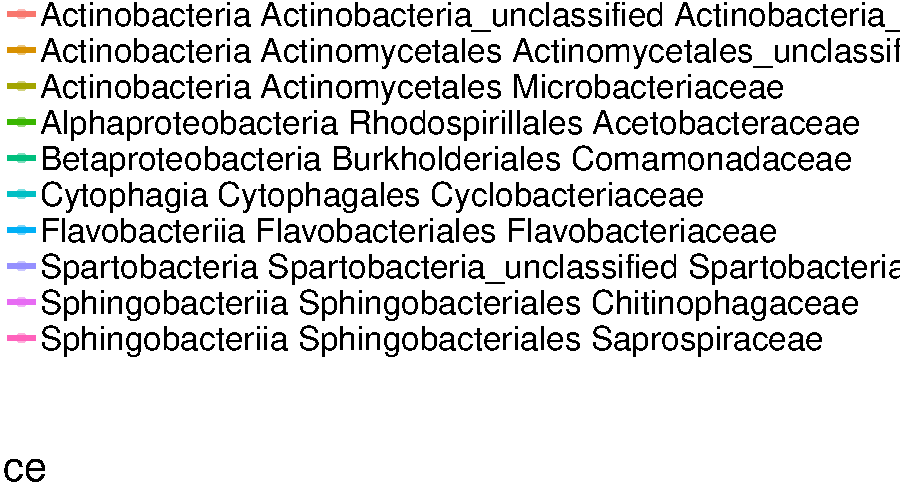
\includegraphics[width=0.7\linewidth]{ReservoirGradient_files/figure-latex/unnamed-chunk-4-4} \end{center}

\begin{Shaded}
\begin{Highlighting}[]
\CommentTok{# how much do the different core components contribute to total abundances}
\NormalTok{in.lake.core.soil.REL <-}\StringTok{ }\KeywordTok{rowSums}\NormalTok{(in.lake.core.from.soils) }\OperatorTok{/}\StringTok{ }\KeywordTok{rowSums}\NormalTok{(w.dna)}
\NormalTok{in.lake.core.water.REL <-}\StringTok{ }\KeywordTok{rowSums}\NormalTok{(in.lake.core.not.soils) }\OperatorTok{/}\StringTok{ }\KeywordTok{rowSums}\NormalTok{(w.dna)}
\end{Highlighting}
\end{Shaded}

\subsection{Taxonomic Analysis}\label{taxonomic-analysis}

\begin{Shaded}
\begin{Highlighting}[]
\CommentTok{# Taxa comprising total lake 'core', those from soils, and those not from soils}
\NormalTok{core.taxa <-}\StringTok{ }\NormalTok{OTU.tax[OTU.tax}\OperatorTok{$}\NormalTok{OTU }\OperatorTok\StringTok{ }\KeywordTok{colnames}\NormalTok{(in.lake.core),]}

\NormalTok{core.soil.taxa <-}\StringTok{ }\NormalTok{OTU.tax[OTU.tax}\OperatorTok{$}\NormalTok{OTU }\OperatorTok\StringTok{ }\KeywordTok{colnames}\NormalTok{(in.lake.core.from.soils),]}
\NormalTok{core.water.taxa <-}\StringTok{ }\NormalTok{OTU.tax[OTU.tax}\OperatorTok{$}\NormalTok{OTU }\OperatorTok\StringTok{ }\KeywordTok{colnames}\NormalTok{(in.lake.core.not.soils),]}

\CommentTok{# Get relative abundances for each of the core taxa }
\NormalTok{core.soil.taxa.DNA.REL <-}\StringTok{ }\NormalTok{OTUsREL[}\KeywordTok{which}\NormalTok{(design}\OperatorTok{$}\NormalTok{molecule }\OperatorTok{==}\StringTok{ "DNA"} \OperatorTok{&}\StringTok{ }\NormalTok{design}\OperatorTok{$}\NormalTok{type }\OperatorTok{==}\StringTok{ "water"}\NormalTok{),}
                                  \KeywordTok{as.numeric}\NormalTok{(}\KeywordTok{rownames}\NormalTok{(core.soil.taxa))]}
\NormalTok{core.water.taxa.DNA.REL <-}\StringTok{ }\NormalTok{OTUsREL[}\KeywordTok{which}\NormalTok{(design}\OperatorTok{$}\NormalTok{molecule }\OperatorTok{==}\StringTok{ "DNA"} \OperatorTok{&}\StringTok{ }\NormalTok{design}\OperatorTok{$}\NormalTok{type }\OperatorTok{==}\StringTok{ "water"}\NormalTok{),}
                                   \KeywordTok{as.numeric}\NormalTok{(}\KeywordTok{rownames}\NormalTok{(core.water.taxa))]}
\NormalTok{core.soil.taxa.RNA.REL <-}\StringTok{ }\NormalTok{OTUsREL[}\KeywordTok{which}\NormalTok{(design}\OperatorTok{$}\NormalTok{molecule }\OperatorTok{==}\StringTok{ "RNA"} \OperatorTok{&}\StringTok{ }\NormalTok{design}\OperatorTok{$}\NormalTok{type }\OperatorTok{==}\StringTok{ "water"}\NormalTok{),}
                                  \KeywordTok{as.numeric}\NormalTok{(}\KeywordTok{rownames}\NormalTok{(core.soil.taxa))]}
\NormalTok{core.water.taxa.RNA.REL <-}\StringTok{ }\NormalTok{OTUsREL[}\KeywordTok{which}\NormalTok{(design}\OperatorTok{$}\NormalTok{molecule }\OperatorTok{==}\StringTok{ "RNA"} \OperatorTok{&}\StringTok{ }\NormalTok{design}\OperatorTok{$}\NormalTok{type }\OperatorTok{==}\StringTok{ "water"}\NormalTok{),}
                                   \KeywordTok{as.numeric}\NormalTok{(}\KeywordTok{rownames}\NormalTok{(core.water.taxa))]}

\NormalTok{core.soil.taxa.DNA.REL.max <-}\StringTok{ }\KeywordTok{as.matrix}\NormalTok{(}\KeywordTok{apply}\NormalTok{(core.soil.taxa.DNA.REL, }\DecValTok{2}\NormalTok{, max))}
\NormalTok{core.soil.taxa.RNA.REL.max <-}\StringTok{ }\KeywordTok{as.matrix}\NormalTok{(}\KeywordTok{apply}\NormalTok{(core.soil.taxa.RNA.REL, }\DecValTok{2}\NormalTok{, max))}
\NormalTok{core.water.taxa.DNA.REL.max <-}\StringTok{ }\KeywordTok{as.matrix}\NormalTok{(}\KeywordTok{apply}\NormalTok{(core.water.taxa.DNA.REL, }\DecValTok{2}\NormalTok{, max))}
\NormalTok{core.water.taxa.RNA.REL.max <-}\StringTok{ }\KeywordTok{as.matrix}\NormalTok{(}\KeywordTok{apply}\NormalTok{(core.water.taxa.RNA.REL, }\DecValTok{2}\NormalTok{, max))}

\NormalTok{core.soil.taxa.DNA.REL.min <-}\StringTok{ }\KeywordTok{as.matrix}\NormalTok{(}\KeywordTok{apply}\NormalTok{(core.soil.taxa.DNA.REL, }\DecValTok{2}\NormalTok{, min))}
\NormalTok{core.soil.taxa.RNA.REL.min <-}\StringTok{ }\KeywordTok{as.matrix}\NormalTok{(}\KeywordTok{apply}\NormalTok{(core.soil.taxa.RNA.REL, }\DecValTok{2}\NormalTok{, min))}
\NormalTok{core.water.taxa.DNA.REL.min <-}\StringTok{ }\KeywordTok{as.matrix}\NormalTok{(}\KeywordTok{apply}\NormalTok{(core.water.taxa.DNA.REL, }\DecValTok{2}\NormalTok{, min))}
\NormalTok{core.water.taxa.RNA.REL.min <-}\StringTok{ }\KeywordTok{as.matrix}\NormalTok{(}\KeywordTok{apply}\NormalTok{(core.water.taxa.RNA.REL, }\DecValTok{2}\NormalTok{, min))}

\NormalTok{core.soil.taxa.DNA.REL.mean <-}\StringTok{ }\KeywordTok{as.matrix}\NormalTok{(}\KeywordTok{apply}\NormalTok{(core.soil.taxa.DNA.REL, }\DecValTok{2}\NormalTok{, mean))}
\NormalTok{core.soil.taxa.RNA.REL.mean <-}\StringTok{ }\KeywordTok{as.matrix}\NormalTok{(}\KeywordTok{apply}\NormalTok{(core.soil.taxa.RNA.REL, }\DecValTok{2}\NormalTok{, mean))}
\NormalTok{core.water.taxa.DNA.REL.mean <-}\StringTok{ }\KeywordTok{as.matrix}\NormalTok{(}\KeywordTok{apply}\NormalTok{(core.water.taxa.DNA.REL, }\DecValTok{2}\NormalTok{, mean))}
\NormalTok{core.water.taxa.RNA.REL.mean <-}\StringTok{ }\KeywordTok{as.matrix}\NormalTok{(}\KeywordTok{apply}\NormalTok{(core.water.taxa.RNA.REL, }\DecValTok{2}\NormalTok{, mean))}

\NormalTok{core.soil.taxa.soil.max <-}\StringTok{ }\KeywordTok{as.matrix}\NormalTok{(}\KeywordTok{apply}\NormalTok{(OTUsREL[}\KeywordTok{which}\NormalTok{(design}\OperatorTok{$}\NormalTok{type }\OperatorTok{==}\StringTok{ "soil"}\NormalTok{), }\KeywordTok{rownames}\NormalTok{(core.soil.taxa.DNA.REL.max)], }\DataTypeTok{MARGIN =} \DecValTok{2}\NormalTok{, max))}

\NormalTok{core.soil.taxa.DNA.REL.bounds <-}\StringTok{ }\KeywordTok{cbind}\NormalTok{(core.soil.taxa.DNA.REL.min, core.soil.taxa.DNA.REL.max,}
\NormalTok{                                       core.soil.taxa.RNA.REL.min, core.soil.taxa.RNA.REL.max,}
\NormalTok{                                       core.soil.taxa.DNA.REL.mean, core.soil.taxa.RNA.REL.mean, }
\NormalTok{                                       core.soil.taxa.soil.max)}

\KeywordTok{colnames}\NormalTok{(core.soil.taxa.DNA.REL.bounds) <-}\StringTok{ }\KeywordTok{c}\NormalTok{(}\StringTok{"DNA.min"}\NormalTok{, }\StringTok{"DNA.max"}\NormalTok{, }\StringTok{"RNA.min"}\NormalTok{, }\StringTok{"RNA.max"}\NormalTok{, }\StringTok{"DNA.mean"}\NormalTok{, }\StringTok{"RNA.mean"}\NormalTok{, }\StringTok{"Soil.max"}\NormalTok{)}




\NormalTok{core.water.taxa.DNA.REL.bounds <-}\StringTok{ }\KeywordTok{cbind}\NormalTok{(core.water.taxa.DNA.REL.min, core.water.taxa.DNA.REL.max,}
\NormalTok{                                       core.water.taxa.RNA.REL.min, core.water.taxa.RNA.REL.max,}
\NormalTok{                                       core.water.taxa.DNA.REL.mean, core.water.taxa.RNA.REL.mean)}
\KeywordTok{colnames}\NormalTok{(core.water.taxa.DNA.REL.bounds) <-}\StringTok{ }\KeywordTok{c}\NormalTok{(}\StringTok{"DNA.min"}\NormalTok{, }\StringTok{"DNA.max"}\NormalTok{, }\StringTok{"RNA.min"}\NormalTok{, }\StringTok{"RNA.max"}\NormalTok{, }\StringTok{"DNA.mean"}\NormalTok{, }\StringTok{"RNA.mean"}\NormalTok{)}

\CommentTok{# core.soil and core.water are summaries of lake core}
\NormalTok{core.soil <-}\StringTok{ }\KeywordTok{as.data.frame}\NormalTok{(}\KeywordTok{cbind}\NormalTok{(core.soil.taxa}\OperatorTok{$}\NormalTok{Family, core.soil.taxa}\OperatorTok{$}\NormalTok{Genus,}
                                 \KeywordTok{signif}\NormalTok{(core.soil.taxa.DNA.REL.bounds[,}\KeywordTok{c}\NormalTok{(}\DecValTok{1}\OperatorTok{:}\DecValTok{4}\NormalTok{, }\DecValTok{7}\NormalTok{)], }\DataTypeTok{digits =} \DecValTok{3}\NormalTok{)))}
\KeywordTok{colnames}\NormalTok{(core.soil) <-}\StringTok{ }\KeywordTok{c}\NormalTok{(}\StringTok{"Family"}\NormalTok{, }\StringTok{"Genus"}\NormalTok{, }\StringTok{"DNA.min"}\NormalTok{, }\StringTok{"DNA.max"}\NormalTok{, }\StringTok{"RNA.min"}\NormalTok{, }\StringTok{"RNA.max"}\NormalTok{, }\StringTok{"Soil.max"}\NormalTok{)}
\NormalTok{core.water <-}\StringTok{ }\KeywordTok{as.data.frame}\NormalTok{(}\KeywordTok{cbind}\NormalTok{(core.water.taxa}\OperatorTok{$}\NormalTok{Family, core.water.taxa}\OperatorTok{$}\NormalTok{Genus, }
                                  \KeywordTok{signif}\NormalTok{(core.water.taxa.DNA.REL.bounds[,}\DecValTok{1}\OperatorTok{:}\DecValTok{4}\NormalTok{], }\DataTypeTok{digits =} \DecValTok{3}\NormalTok{)))}
\KeywordTok{colnames}\NormalTok{(core.water) <-}\StringTok{ }\KeywordTok{c}\NormalTok{(}\StringTok{"Family"}\NormalTok{, }\StringTok{"Genus"}\NormalTok{, }\StringTok{"DNA.min"}\NormalTok{, }\StringTok{"DNA.max"}\NormalTok{, }\StringTok{"RNA.min"}\NormalTok{, }\StringTok{"RNA.max"}\NormalTok{)}

\CommentTok{# Core Soil LaTeX Table}
\NormalTok{addtorow <-}\StringTok{ }\KeywordTok{list}\NormalTok{()}
\NormalTok{addtorow}\OperatorTok{$}\NormalTok{pos <-}\StringTok{ }\KeywordTok{list}\NormalTok{(}\DecValTok{0}\NormalTok{, }\DecValTok{0}\NormalTok{)}
\NormalTok{addtorow}\OperatorTok{$}\NormalTok{command <-}\StringTok{ }\KeywordTok{c}\NormalTok{(}\StringTok{"& }\CharTok{\textbackslash{}\textbackslash{}}\StringTok{multicolumn\{1\}\{c\}\{Class\} & }\CharTok{\textbackslash{}\textbackslash{}}\StringTok{multicolumn\{1\}\{c\}\{Order\} & }
\StringTok{                      }\CharTok{\textbackslash{}\textbackslash{}}\StringTok{multicolumn\{2\}\{c\}\{DNA\} & }\CharTok{\textbackslash{}\textbackslash{}}\StringTok{multicolumn\{2\}\{c\}\{RNA\} }\CharTok{\textbackslash{}\textbackslash{}\textbackslash{}\textbackslash{}\textbackslash{}n}\StringTok{"}\NormalTok{, }
                      \StringTok{"& &  & min & max & min & max }\CharTok{\textbackslash{}\textbackslash{}\textbackslash{}\textbackslash{}\textbackslash{}n}\StringTok{"}\NormalTok{)}
\NormalTok{core.soil.tab <-}\StringTok{ }\KeywordTok{xtable}\NormalTok{(core.soil)}
\KeywordTok{align}\NormalTok{(core.soil.tab) <-}\StringTok{ "crrrrrrr"}
\KeywordTok{print}\NormalTok{(core.soil.tab, }\DataTypeTok{add.to.row =}\NormalTok{ addtorow, }\DataTypeTok{include.colnames =} \OtherTok{FALSE}\NormalTok{, }
      \DataTypeTok{type=} \StringTok{"latex"}\NormalTok{, }\DataTypeTok{file=}\StringTok{"tables/table1.tex"}\NormalTok{)}
\KeywordTok{print}\NormalTok{(core.soil.tab, }\DataTypeTok{add.to.row =}\NormalTok{ addtorow, }\DataTypeTok{include.colnames =} \OtherTok{FALSE}\NormalTok{, }\DataTypeTok{comment =} \OtherTok{FALSE}\NormalTok{)}
\end{Highlighting}
\end{Shaded}

\begin{table}[ht]
\centering
\begin{tabular}{crrrrrrr}
  \hline
  & \multicolumn{1}{c}{Class} & \multicolumn{1}{c}{Order} & 
                      \multicolumn{2}{c}{DNA} & \multicolumn{2}{c}{RNA} \\
 & &  & min & max & min & max \\
 \hline
Otu00001 & Comamonadaceae & Comamonadaceae\_unclassified & 0.00465 & 0.026 & 5.1e-05 & 0.0906 & 0.00348 \\ 
  Otu00002 & Actinomycetales\_unclassified & Actinomycetales\_unclassified & 0.00327 & 0.127 & 0 & 0.142 & 1.45e-05 \\ 
  Otu00003 & Spartobacteria\_unclassified & Spartobacteria\_unclassified & 0.0016 & 0.06 & 2.69e-05 & 0.161 & 2.42e-05 \\ 
  Otu00005 & Chitinophagaceae & Sediminibacterium & 0.00155 & 0.0369 & 0 & 0.0789 & 0.000295 \\ 
  Otu00006 & Saprospiraceae & Saprospiraceae\_unclassified & 0.000158 & 0.00806 & 0 & 0.107 & 1.45e-05 \\ 
  Otu00008 & Actinomycetales\_unclassified & Actinomycetales\_unclassified & 0.000716 & 0.0288 & 0 & 0.0707 & 9.68e-06 \\ 
  Otu00009 & Pseudomonadaceae & Pseudomonas & 0 & 0.0412 & 3.1e-05 & 0.271 & 0.00046 \\ 
  Otu00010 & Proteobacteria\_unclassified & Proteobacteria\_unclassified & 0.00297 & 0.134 & 4.25e-05 & 0.0481 & 1.94e-05 \\ 
  Otu00011 & Betaproteobacteria\_unclassified & Betaproteobacteria\_unclassified & 0.000108 & 0.0731 & 5.23e-06 & 0.0908 & 6.27e-06 \\ 
  Otu00012 & Comamonadaceae & Comamonadaceae\_unclassified & 0.00616 & 0.0186 & 8.5e-06 & 0.28 & 0.00268 \\ 
  Otu00014 & Actinomycetales\_unclassified & Actinomycetales\_unclassified & 0.00108 & 0.0512 & 0 & 0.0524 & 6.27e-06 \\ 
  Otu00015 & Actinobacteria\_unclassified & Actinobacteria\_unclassified & 0.000363 & 0.0675 & 0 & 0.0127 & 1.45e-05 \\ 
  Otu00016 & Microbacteriaceae & Microbacteriaceae\_unclassified & 0.000115 & 0.0268 & 0 & 0.03 & 4.83e-06 \\ 
  Otu00017 & Actinomycetales\_unclassified & Actinomycetales\_unclassified & 0.00103 & 0.0141 & 0 & 0.055 & 9.68e-06 \\ 
  Otu00018 & Pseudomonadaceae & Pseudomonas & 4.21e-05 & 0.0328 & 3.12e-05 & 0.495 & 0.000232 \\ 
  Otu00019 & Cytophagaceae & Cytophagaceae\_unclassified & 0.000697 & 0.0844 & 0 & 0.0126 & 1.45e-05 \\ 
  Otu00020 & Alcaligenaceae & Alcaligenaceae\_unclassified & 0.000777 & 0.0399 & 0 & 0.15 & 4.83e-06 \\ 
  Otu00022 & Opitutae\_unclassified & Opitutae\_unclassified & 0.00421 & 0.0332 & 5.23e-06 & 0.277 & 9.68e-06 \\ 
  Otu00023 & Moraxellaceae & Acinetobacter & 0 & 0.00186 & 1.55e-05 & 0.862 & 1.93e-05 \\ 
  Otu00024 & Bacteroidetes\_unclassified & Bacteroidetes\_unclassified & 0.000367 & 0.00679 & 0 & 0.0448 & 4.84e-06 \\ 
  Otu00025 & Microbacteriaceae & Microbacteriaceae\_unclassified & 0.00233 & 0.0271 & 0 & 0.0978 & 9.68e-06 \\ 
  Otu00028 & Pseudomonadaceae & Pseudomonas & 0 & 0.0232 & 5.23e-06 & 0.288 & 0.00227 \\ 
  Otu00030 & Micrococcaceae & Micrococcus & 6.84e-05 & 0.0215 & 1.56e-05 & 0.734 & 2.41e-05 \\ 
  Otu00031 & Cyclobacteriaceae & Algoriphagus & 0.000735 & 0.0293 & 0 & 0.0594 & 4.84e-06 \\ 
  Otu00032 & Bacteroidetes\_unclassified & Bacteroidetes\_unclassified & 0.00101 & 0.0326 & 0 & 0.279 & 6.27e-06 \\ 
  Otu00033 & Rhizobiales\_unclassified & Rhizobiales\_unclassified & 0.00136 & 0.0398 & 5.16e-06 & 0.209 & 0.000136 \\ 
  Otu00039 & Comamonadaceae & Comamonas & 0.000143 & 0.0142 & 0 & 0.0494 & 8.78e-05 \\ 
  Otu00040 & Acetobacteraceae & Roseomonas & 0.00021 & 0.015 & 0 & 0.19 & 9.66e-06 \\ 
  Otu00042 & Burkholderiaceae & Burkholderia & 0 & 0.0129 & 0 & 0.385 & 0.00311 \\ 
  Otu00045 & Oxalobacteraceae & Oxalobacteraceae\_unclassified & 0.00103 & 0.0214 & 0 & 0.00368 & 0.000864 \\ 
  Otu00053 & Clostridiales\_Incertae\_Sedis\_XI & Finegoldia & 0 & 0.00102 & 0 & 0.446 & 6.27e-06 \\ 
  Otu00057 & Methylococcaceae & Methylococcaceae\_unclassified & 0.000373 & 0.0179 & 0 & 0.0649 & 1.25e-05 \\ 
  Otu00059 & Micrococcaceae & Arthrobacter & 0 & 0.0435 & 0 & 0.00456 & 0.000343 \\ 
  Otu00063 & Verrucomicrobia\_unclassified & Verrucomicrobia\_unclassified & 0.000573 & 0.0317 & 0 & 0.0676 & 9.66e-06 \\ 
  Otu00065 & Sphingobacteriaceae & Pedobacter & 0 & 0.0344 & 0 & 0.0042 & 0.000194 \\ 
  Otu00069 & Xanthomonadaceae & Stenotrophomonas & 0 & 0.000679 & 0 & 0.388 & 9.66e-06 \\ 
  Otu00072 & Sphingomonadaceae & Sphingomonas & 7.52e-05 & 0.118 & 0 & 0.0672 & 0.000853 \\ 
  Otu00078 & Flavobacteriaceae & Flavobacterium & 5.63e-06 & 0.00306 & 0 & 0.00533 & 0.000232 \\ 
  Otu00081 & Flavobacteriaceae & Flavobacterium & 0 & 0.0154 & 0 & 0.00224 & 0.000157 \\ 
  Otu00082 & Oxalobacteraceae & Janthinobacterium & 0.000957 & 0.0141 & 0 & 0.0115 & 0 \\ 
  Otu00087 & Bradyrhizobiaceae & Bradyrhizobium & 7.74e-06 & 0.000906 & 0 & 0.00024 & 0.000232 \\ 
  Otu00089 & Sphingobacteriales\_unclassified & Sphingobacteriales\_unclassified & 3.82e-05 & 0.0163 & 0 & 0.0136 & 0 \\ 
  Otu00094 & Sphingobacteriaceae & Sphingobacterium & 0 & 0.0142 & 0 & 0.00125 & 0.000439 \\ 
  Otu00095 & Oxalobacteraceae & Duganella & 4.56e-05 & 0.0269 & 5.23e-06 & 0.0391 & 0.000364 \\ 
  Otu00098 & Sphingomonadaceae & Sphingomonadaceae\_unclassified & 0 & 0.00101 & 0 & 0.000198 & 0.00301 \\ 
  Otu00118 & Comamonadaceae & Comamonadaceae\_unclassified & 0.00023 & 0.00495 & 0 & 0.0204 & 0 \\ 
  Otu00144 & Methylococcaceae & Methylobacter & 0 & 0.000353 & 0 & 8.86e-06 & 0.000121 \\ 
  Otu00145 & Caulobacteraceae & Phenylobacterium & 0 & 0.00107 & 0 & 1.12e-05 & 4.83e-06 \\ 
  Otu00158 & Sphingomonadaceae & Sphingomonas & 0 & 0.000484 & 0 & 0.000127 & 6.29e-05 \\ 
  Otu00162 & Aeromonadaceae & Aeromonas & 0 & 0.000611 & 0 & 7.07e-05 & 0 \\ 
  Otu00279 & Rhizobiaceae & Rhizobiaceae\_unclassified & 7.74e-06 & 0.00201 & 0 & 0.0175 & 0 \\ 
  Otu00838 & Chitinophagaceae & Chitinophagaceae\_unclassified & 0 & 0.000162 & 0 & 0.000368 & 0 \\ 
  Otu01248 & Subdivision3\_unclassified & Subdivision3\_unclassified & 0 & 2.87e-05 & 0 & 1.78e-05 & 0 \\ 
   \hline
\end{tabular}
\end{table}

\begin{Shaded}
\begin{Highlighting}[]
\NormalTok{core.water.tab <-}\StringTok{ }\KeywordTok{xtable}\NormalTok{(core.water)}
\KeywordTok{align}\NormalTok{(core.water.tab) <-}\StringTok{ "crrrrrr"}
\KeywordTok{print}\NormalTok{(core.water.tab, }\DataTypeTok{add.to.row =}\NormalTok{ addtorow, }\DataTypeTok{include.colnames =} \OtherTok{FALSE}\NormalTok{, }
      \DataTypeTok{type=} \StringTok{"latex"}\NormalTok{, }\DataTypeTok{file=}\StringTok{"tables/table2.tex"}\NormalTok{)}
\KeywordTok{print}\NormalTok{(core.water.tab, }\DataTypeTok{add.to.row =}\NormalTok{ addtorow, }\DataTypeTok{include.colnames =} \OtherTok{FALSE}\NormalTok{, }\DataTypeTok{comment =} \OtherTok{FALSE}\NormalTok{)}
\end{Highlighting}
\end{Shaded}

\begin{table}[ht]
\centering
\begin{tabular}{crrrrrr}
  \hline
  & \multicolumn{1}{c}{Class} & \multicolumn{1}{c}{Order} & 
                      \multicolumn{2}{c}{DNA} & \multicolumn{2}{c}{RNA} \\
 & &  & min & max & min & max \\
 \hline
Otu00004 & Actinomycetales\_unclassified & Actinomycetales\_unclassified & 0.00348 & 0.0602 & 0 & 0.0227 \\ 
  Otu00007 & Burkholderiaceae & Polynucleobacter & 0.000697 & 0.0207 & 0 & 0.0865 \\ 
  Otu00038 & Actinomycetales\_unclassified & Actinomycetales\_unclassified & 0.00153 & 0.0222 & 0 & 0.0986 \\ 
  Otu00080 & Bacteroidetes\_unclassified & Bacteroidetes\_unclassified & 1.91e-05 & 0.0189 & 0 & 0.0188 \\ 
  Otu00090 & Opitutae\_unclassified & Opitutae\_unclassified & 0 & 0.00123 & 0 & 0.187 \\ 
  Otu00136 & Methylococcaceae & Methylomonas & 0 & 0.00192 & 0 & 0.0121 \\ 
  Otu00140 & Cryomorphaceae & Fluviicola & 0 & 0.000679 & 0 & 0.15 \\ 
  Otu00142 & Bacteroidetes\_unclassified & Bacteroidetes\_unclassified & 0.000101 & 0.0053 & 0 & 0.0537 \\ 
  Otu00172 & Bacteroidetes\_unclassified & Bacteroidetes\_unclassified & 9.55e-06 & 0.00224 & 0 & 0.00231 \\ 
  Otu00173 & Bacteria\_unclassified & Bacteria\_unclassified & 0 & 0.000459 & 0 & 0 \\ 
  Otu00532 & Bacteroidetes\_unclassified & Bacteroidetes\_unclassified & 0 & 0.000772 & 0 & 0.000571 \\ 
  Otu00633 & Nitrosomonadaceae & Nitrosomonas & 0 & 0.000561 & 0 & 2.69e-05 \\ 
  Otu01046 & Clostridiales\_Incertae\_Sedis\_XI & Anaerococcus & 0 & 6.54e-05 & 0 & 1.41e-05 \\ 
  Otu01198 & Burkholderiales\_unclassified & Burkholderiales\_unclassified & 0 & 0.000274 & 0 & 4.24e-05 \\ 
   \hline
\end{tabular}
\end{table}

\subsection{Comparisons of relabunds}\label{comparisons-of-relabunds}

Now, lets see which taxa increase or decrease substantially along the
gradient. I calculated the fold change in relative abundance of all
these taxa along the gradient relative to their max abundance in soils.
Thus, the OTUs that are most abundant near the soils will have a
declining slope toward the dam. The OTUs that are perhaps seeded from
the soils into the lake will have an increasing slope toward the dam.

\begin{Shaded}
\begin{Highlighting}[]
\NormalTok{high.activity.soil.core <-}\StringTok{ }\KeywordTok{as.data.frame}\NormalTok{(core.soil.taxa.DNA.REL.bounds) }\OperatorTok
\StringTok{  }\KeywordTok{rownames_to_column}\NormalTok{(}\StringTok{"OTU"}\NormalTok{) }\OperatorTok\StringTok{ }
\StringTok{  }\KeywordTok{filter}\NormalTok{(RNA.max }\OperatorTok{>}\StringTok{ }\DecValTok{0}\NormalTok{) }\OperatorTok\StringTok{ }\KeywordTok{arrange}\NormalTok{(}\KeywordTok{desc}\NormalTok{(RNA.max)) }\OperatorTok\StringTok{ }
\StringTok{  }\KeywordTok{left_join}\NormalTok{(OTU.tax)}
\end{Highlighting}
\end{Shaded}

\begin{verbatim}
## Warning: Column `OTU` joining character vector and factor, coercing into
## character vector
\end{verbatim}

\begin{Shaded}
\begin{Highlighting}[]
\NormalTok{high.activity.water.core <-}\StringTok{ }\KeywordTok{as.data.frame}\NormalTok{(core.water.taxa.DNA.REL.bounds) }\OperatorTok
\StringTok{  }\KeywordTok{rownames_to_column}\NormalTok{(}\StringTok{"OTU"}\NormalTok{) }\OperatorTok\StringTok{ }
\StringTok{  }\KeywordTok{filter}\NormalTok{(RNA.max }\OperatorTok{>}\StringTok{ }\DecValTok{0}\NormalTok{) }\OperatorTok\StringTok{ }\KeywordTok{arrange}\NormalTok{(}\KeywordTok{desc}\NormalTok{(RNA.max)) }\OperatorTok\StringTok{ }
\StringTok{  }\KeywordTok{left_join}\NormalTok{(OTU.tax)}
\end{Highlighting}
\end{Shaded}

\begin{verbatim}
## Warning: Column `OTU` joining character vector and factor, coercing into
## character vector
\end{verbatim}

\begin{Shaded}
\begin{Highlighting}[]
\NormalTok{mean.soil.abunds.soil.core <-}\StringTok{ }\NormalTok{OTUsREL[}\KeywordTok{which}\NormalTok{(design}\OperatorTok{$}\NormalTok{type }\OperatorTok{==}\StringTok{ "soil"}\NormalTok{), high.activity.soil.core}\OperatorTok{$}\NormalTok{OTU] }\OperatorTok\StringTok{ }
\StringTok{  }\NormalTok{colMeans }\OperatorTok\StringTok{ }\KeywordTok{data.frame}\NormalTok{(}\DataTypeTok{mean_soil_relabund =}\NormalTok{ .) }\OperatorTok\StringTok{ }
\StringTok{  }\KeywordTok{rownames_to_column}\NormalTok{(}\StringTok{"OTU"}\NormalTok{) }\OperatorTok\StringTok{ }\KeywordTok{arrange}\NormalTok{(}\KeywordTok{desc}\NormalTok{(mean_soil_relabund))}
\NormalTok{max.soil.abunds.soil.core <-}\StringTok{ }\NormalTok{OTUsREL[}\KeywordTok{which}\NormalTok{(design}\OperatorTok{$}\NormalTok{type }\OperatorTok{==}\StringTok{ "soil"}\NormalTok{), high.activity.soil.core}\OperatorTok{$}\NormalTok{OTU] }\OperatorTok\StringTok{ }
\StringTok{  }\KeywordTok{apply}\NormalTok{(}\DataTypeTok{X =}\NormalTok{ ., }\DataTypeTok{MARGIN =} \DecValTok{2}\NormalTok{, max) }\OperatorTok\StringTok{ }\KeywordTok{data.frame}\NormalTok{(}\DataTypeTok{max_soil_relabund =}\NormalTok{ .) }\OperatorTok\StringTok{ }
\StringTok{  }\KeywordTok{rownames_to_column}\NormalTok{(}\StringTok{"OTU"}\NormalTok{) }\OperatorTok\StringTok{ }\KeywordTok{arrange}\NormalTok{(}\KeywordTok{desc}\NormalTok{(max_soil_relabund))}

\NormalTok{mean.soil.abunds.water.core <-}\StringTok{ }\NormalTok{OTUsREL[}\KeywordTok{which}\NormalTok{(design}\OperatorTok{$}\NormalTok{type }\OperatorTok{==}\StringTok{ "soil"}\NormalTok{), high.activity.water.core}\OperatorTok{$}\NormalTok{OTU] }\OperatorTok\StringTok{ }
\StringTok{  }\NormalTok{colMeans }\OperatorTok\StringTok{ }\KeywordTok{data.frame}\NormalTok{(}\DataTypeTok{mean_soil_relabund =}\NormalTok{ .) }\OperatorTok\StringTok{ }
\StringTok{  }\KeywordTok{rownames_to_column}\NormalTok{(}\StringTok{"OTU"}\NormalTok{) }\OperatorTok\StringTok{ }\KeywordTok{arrange}\NormalTok{(}\KeywordTok{desc}\NormalTok{(mean_soil_relabund))}
\NormalTok{max.soil.abunds.water.core <-}\StringTok{ }\NormalTok{OTUsREL[}\KeywordTok{which}\NormalTok{(design}\OperatorTok{$}\NormalTok{type }\OperatorTok{==}\StringTok{ "soil"}\NormalTok{), high.activity.water.core}\OperatorTok{$}\NormalTok{OTU] }\OperatorTok\StringTok{ }
\StringTok{  }\KeywordTok{apply}\NormalTok{(}\DataTypeTok{X =}\NormalTok{ ., }\DataTypeTok{MARGIN =} \DecValTok{2}\NormalTok{, max) }\OperatorTok\StringTok{ }\KeywordTok{data.frame}\NormalTok{(}\DataTypeTok{max_soil_relabund =}\NormalTok{ .) }\OperatorTok\StringTok{ }
\StringTok{  }\KeywordTok{rownames_to_column}\NormalTok{(}\StringTok{"OTU"}\NormalTok{) }\OperatorTok\StringTok{ }\KeywordTok{arrange}\NormalTok{(}\KeywordTok{desc}\NormalTok{(max_soil_relabund))}


\NormalTok{soil.vs.lake.abunds <-}\StringTok{ }\NormalTok{high.activity.soil.core }\OperatorTok\StringTok{ }
\StringTok{  }\KeywordTok{left_join}\NormalTok{(mean.soil.abunds.soil.core) }\OperatorTok\StringTok{ }\KeywordTok{left_join}\NormalTok{(max.soil.abunds.soil.core) }\OperatorTok\StringTok{ }
\StringTok{  }\KeywordTok{mutate}\NormalTok{(}\DataTypeTok{soil_is_source =} \KeywordTok{ifelse}\NormalTok{(max_soil_relabund }\OperatorTok{>}\StringTok{ }\FloatTok{1e-3} \OperatorTok{&}\StringTok{ }\NormalTok{RNA.max }\OperatorTok{>}\StringTok{ }\FloatTok{1e-3}\NormalTok{, T, F)) }\OperatorTok\StringTok{ }
\StringTok{  }\KeywordTok{mutate}\NormalTok{(}\DataTypeTok{Taxon =} \KeywordTok{ifelse}\NormalTok{(Genus }\OperatorTok{==}\StringTok{ "unclassified"}\NormalTok{, }\KeywordTok{paste}\NormalTok{(Family, }\StringTok{"sp."}\NormalTok{), Genus))}

\NormalTok{combined.relabunds <-}\StringTok{ }\NormalTok{max.soil.abunds.soil.core }\OperatorTok
\StringTok{  }\KeywordTok{left_join}\NormalTok{(}\KeywordTok{rownames_to_column}\NormalTok{(}\KeywordTok{as.data.frame}\NormalTok{(}\KeywordTok{t}\NormalTok{(in.lake.core.from.soils.REL)), }\StringTok{"OTU"}\NormalTok{))}
\KeywordTok{rownames}\NormalTok{(combined.relabunds) <-}\StringTok{ }\NormalTok{combined.relabunds}\OperatorTok{$}\NormalTok{OTU}
\NormalTok{combined.relabunds <-}\StringTok{ }\NormalTok{combined.relabunds[,}\OperatorTok{-}\DecValTok{1}\NormalTok{]}

\NormalTok{otus.fold.change <-}\StringTok{ }\KeywordTok{na.omit}\NormalTok{(combined.relabunds }\OperatorTok{/}\StringTok{ }\NormalTok{combined.relabunds}\OperatorTok{$}\NormalTok{max_soil_relabund) }\CommentTok{# Calculate fold changes}

\NormalTok{fold_change_summary <-}\StringTok{ }\NormalTok{otus.fold.change }\OperatorTok\StringTok{ }\KeywordTok{rownames_to_column}\NormalTok{(}\StringTok{"OTU"}\NormalTok{) }\OperatorTok\StringTok{ }
\StringTok{  }\KeywordTok{select}\NormalTok{(}\OperatorTok{-}\NormalTok{max_soil_relabund) }\OperatorTok\StringTok{ }
\StringTok{  }\KeywordTok{gather}\NormalTok{(}\StringTok{"sample"}\NormalTok{, }\StringTok{"fold_change"}\NormalTok{, }\OperatorTok{-}\NormalTok{OTU) }\OperatorTok\StringTok{ }
\StringTok{  }\KeywordTok{left_join}\NormalTok{(}\KeywordTok{select}\NormalTok{(}\KeywordTok{rownames_to_column}\NormalTok{(design.dna, }\StringTok{"sample"}\NormalTok{), }\OperatorTok{-}\NormalTok{station, }\OperatorTok{-}\NormalTok{molecule, }\OperatorTok{-}\NormalTok{type)) }\OperatorTok\StringTok{ }
\StringTok{  }\KeywordTok{group_by}\NormalTok{(OTU) }\OperatorTok\StringTok{ }
\StringTok{  }\KeywordTok{summarize}\NormalTok{(}\DataTypeTok{max_change =} \KeywordTok{max}\NormalTok{(fold_change), }\DataTypeTok{min_change =} \KeywordTok{min}\NormalTok{(fold_change))}

\NormalTok{otus.fold.change }\OperatorTok\StringTok{ }\KeywordTok{rownames_to_column}\NormalTok{(}\StringTok{"OTU"}\NormalTok{) }\OperatorTok\StringTok{ }
\StringTok{  }\KeywordTok{select}\NormalTok{(}\OperatorTok{-}\NormalTok{max_soil_relabund) }\OperatorTok\StringTok{ }
\StringTok{  }\KeywordTok{gather}\NormalTok{(}\StringTok{"sample"}\NormalTok{, }\StringTok{"fold_change"}\NormalTok{, }\OperatorTok{-}\NormalTok{OTU) }\OperatorTok\StringTok{ }
\StringTok{  }\KeywordTok{left_join}\NormalTok{(}\KeywordTok{select}\NormalTok{(}\KeywordTok{rownames_to_column}\NormalTok{(design.dna, }\StringTok{"sample"}\NormalTok{), }\OperatorTok{-}\NormalTok{station, }\OperatorTok{-}\NormalTok{molecule, }\OperatorTok{-}\NormalTok{type)) }\OperatorTok\StringTok{ }
\StringTok{  }\KeywordTok{ggplot}\NormalTok{(}\KeywordTok{aes}\NormalTok{(}\DataTypeTok{x =}\NormalTok{ distance, }\DataTypeTok{y =}\NormalTok{ fold_change, }\DataTypeTok{color =}\NormalTok{ OTU)) }\OperatorTok{+}\StringTok{ }
\StringTok{  }\KeywordTok{geom_hline}\NormalTok{(}\KeywordTok{aes}\NormalTok{(}\DataTypeTok{yintercept =} \DecValTok{1}\NormalTok{), }\DataTypeTok{color =} \StringTok{"gray50"}\NormalTok{, }\DataTypeTok{alpha =} \FloatTok{0.5}\NormalTok{, }\DataTypeTok{size =} \DecValTok{2}\NormalTok{) }\OperatorTok{+}
\StringTok{  }\KeywordTok{geom_jitter}\NormalTok{(}\DataTypeTok{alpha =} \FloatTok{0.05}\NormalTok{) }\OperatorTok{+}\StringTok{ }
\StringTok{  }\KeywordTok{geom_smooth}\NormalTok{(}\DataTypeTok{alpha =} \FloatTok{0.5}\NormalTok{, }\DataTypeTok{method =} \StringTok{"lm"}\NormalTok{, }\DataTypeTok{se =}\NormalTok{ F) }\OperatorTok{+}\StringTok{ }
\StringTok{  }\KeywordTok{scale_y_log10}\NormalTok{(}\DataTypeTok{labels =}\NormalTok{ scales}\OperatorTok{::}\NormalTok{comma) }\OperatorTok{+}
\StringTok{  }\KeywordTok{scale_x_reverse}\NormalTok{() }\OperatorTok{+}
\StringTok{  }\KeywordTok{annotation_logticks}\NormalTok{(}\DataTypeTok{long =} \KeywordTok{unit}\NormalTok{(.}\DecValTok{1}\NormalTok{, }\StringTok{"in"}\NormalTok{), }\DataTypeTok{sides =} \StringTok{"l"}\NormalTok{) }\OperatorTok{+}
\StringTok{  }\KeywordTok{theme}\NormalTok{(}\DataTypeTok{legend.position =} \StringTok{"none"}\NormalTok{) }\OperatorTok{+}
\StringTok{  }\KeywordTok{labs}\NormalTok{(}\DataTypeTok{x =} \StringTok{"Reservoir Transect (m)"}\NormalTok{, }\DataTypeTok{y =} \StringTok{"Fold-change in abundance"}\NormalTok{)}
\end{Highlighting}
\end{Shaded}

\begin{verbatim}
## Warning: Transformation introduced infinite values in continuous y-axis
\end{verbatim}

\begin{verbatim}
## Warning: Transformation introduced infinite values in continuous y-axis
\end{verbatim}

\begin{verbatim}
## Warning: Removed 42 rows containing non-finite values (stat_smooth).
\end{verbatim}

\begin{center}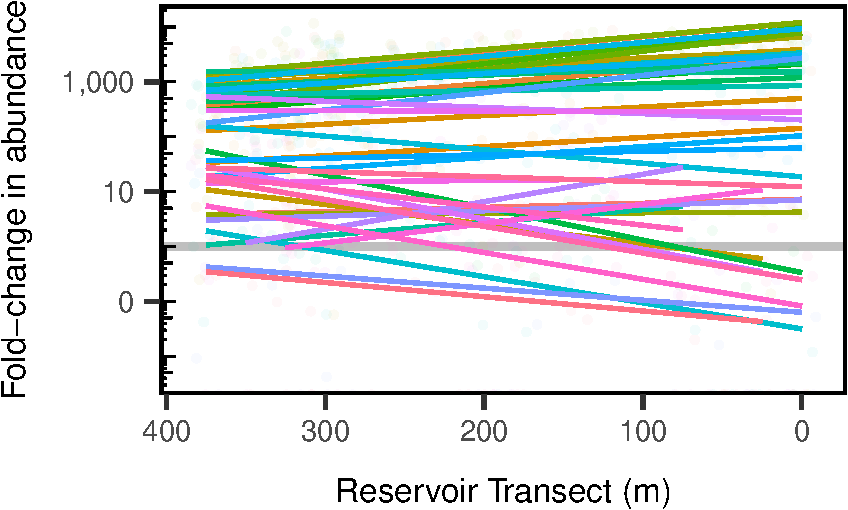
\includegraphics[width=0.7\linewidth]{ReservoirGradient_files/figure-latex/fold_change_plot-1} \end{center}

\begin{Shaded}
\begin{Highlighting}[]
\CommentTok{# otus.fold.change %>% rownames_to_column("OTU") %>% }
\CommentTok{#   select(-max_soil_relabund) %>% }
\CommentTok{#   gather("sample", "fold_change", -OTU) %>% }
\CommentTok{#   left_join(select(rownames_to_column(design.dna, "sample"), -station, -molecule, -type))}

\NormalTok{foldchanges <-}\StringTok{ }\KeywordTok{t}\NormalTok{(otus.fold.change)[}\OperatorTok{-}\DecValTok{1}\NormalTok{,]}
\NormalTok{foldchangelms <-}\StringTok{ }\KeywordTok{apply}\NormalTok{(foldchanges, }\DataTypeTok{MARGIN =} \DecValTok{2}\NormalTok{, }
    \DataTypeTok{FUN =} \ControlFlowTok{function}\NormalTok{(x) }\KeywordTok{summary}\NormalTok{(}\KeywordTok{lm}\NormalTok{(x }\OperatorTok{~}\StringTok{ }\NormalTok{design.dna}\OperatorTok{$}\NormalTok{distance))}\OperatorTok{$}\NormalTok{coefficients[}\KeywordTok{c}\NormalTok{(}\DecValTok{1}\NormalTok{,}\DecValTok{2}\NormalTok{,}\DecValTok{8}\NormalTok{)])}
\KeywordTok{rownames}\NormalTok{(foldchangelms) <-}\StringTok{ }\KeywordTok{c}\NormalTok{(}\StringTok{"intercept"}\NormalTok{, }\StringTok{"slope"}\NormalTok{, }\StringTok{"pval"}\NormalTok{)}

\NormalTok{soil.core.decresing <-}\StringTok{ }\KeywordTok{as.data.frame}\NormalTok{(}\KeywordTok{t}\NormalTok{(foldchangelms)) }\OperatorTok\StringTok{ }
\StringTok{  }\KeywordTok{rownames_to_column}\NormalTok{(}\StringTok{"OTU"}\NormalTok{) }\OperatorTok\StringTok{ }
\StringTok{  }\KeywordTok{filter}\NormalTok{( slope }\OperatorTok{>}\StringTok{ }\DecValTok{0}\NormalTok{) }\OperatorTok\StringTok{   }\CommentTok{# rel abund decreases toward dam}
\StringTok{  }\KeywordTok{left_join}\NormalTok{(OTU.tax) }\OperatorTok\StringTok{ }\KeywordTok{select}\NormalTok{(}\OperatorTok{-}\NormalTok{intercept, }\OperatorTok{-}\NormalTok{slope, }\OperatorTok{-}\NormalTok{pval, }\KeywordTok{everything}\NormalTok{()) }\OperatorTok\StringTok{ }
\StringTok{  }\KeywordTok{arrange}\NormalTok{(}\KeywordTok{desc}\NormalTok{(slope))}
\end{Highlighting}
\end{Shaded}

\begin{verbatim}
## Warning: Column `OTU` joining character vector and factor, coercing into
## character vector
\end{verbatim}

\begin{Shaded}
\begin{Highlighting}[]
\NormalTok{soil.core.increasing <-}\StringTok{ }\KeywordTok{as.data.frame}\NormalTok{(}\KeywordTok{t}\NormalTok{(foldchangelms)) }\OperatorTok\StringTok{ }
\StringTok{  }\KeywordTok{rownames_to_column}\NormalTok{(}\StringTok{"OTU"}\NormalTok{) }\OperatorTok\StringTok{ }
\StringTok{  }\KeywordTok{filter}\NormalTok{( slope }\OperatorTok{<}\StringTok{ }\DecValTok{0}\NormalTok{) }\OperatorTok\StringTok{   }\CommentTok{# rel abund increases toward dam}
\StringTok{  }\KeywordTok{left_join}\NormalTok{(OTU.tax) }\OperatorTok\StringTok{ }\KeywordTok{select}\NormalTok{(}\OperatorTok{-}\NormalTok{intercept, }\OperatorTok{-}\NormalTok{slope, }\OperatorTok{-}\NormalTok{pval, }\KeywordTok{everything}\NormalTok{()) }\OperatorTok\StringTok{ }
\StringTok{  }\KeywordTok{arrange}\NormalTok{((slope))}
\end{Highlighting}
\end{Shaded}

\begin{verbatim}
## Warning: Column `OTU` joining character vector and factor, coercing into
## character vector
\end{verbatim}

\begin{Shaded}
\begin{Highlighting}[]
\NormalTok{soil.decrease.tab <-}\StringTok{ }\NormalTok{soil.core.decresing }\OperatorTok\StringTok{ }\KeywordTok{select}\NormalTok{(}\OperatorTok{-}\NormalTok{OTU, }\OperatorTok{-}\NormalTok{Domain) }\OperatorTok\StringTok{  }\KeywordTok{flextable}\NormalTok{()}
\NormalTok{soil.increase.tab <-}\StringTok{ }\NormalTok{soil.core.increasing }\OperatorTok\StringTok{ }\KeywordTok{select}\NormalTok{(}\OperatorTok{-}\NormalTok{OTU, }\OperatorTok{-}\NormalTok{Domain) }\OperatorTok\StringTok{ }\KeywordTok{flextable}\NormalTok{()}

\KeywordTok{read_docx}\NormalTok{() }\OperatorTok\StringTok{ }
\StringTok{  }\KeywordTok{body_end_section_continuous}\NormalTok{() }\OperatorTok\StringTok{ }
\StringTok{  }\KeywordTok{body_add_par}\NormalTok{(}\StringTok{"Increasing away from stream inlet"}\NormalTok{, }\DataTypeTok{style =} \StringTok{"heading 2"}\NormalTok{) }\OperatorTok\StringTok{ }
\StringTok{  }\KeywordTok{body_add_flextable}\NormalTok{(soil.increase.tab) }\OperatorTok\StringTok{ }
\StringTok{  }\KeywordTok{body_add_par}\NormalTok{(}\StringTok{"Decreasing away from stream inlet"}\NormalTok{, }\DataTypeTok{style =} \StringTok{"heading 2"}\NormalTok{) }\OperatorTok\StringTok{ }
\StringTok{  }\KeywordTok{body_add_flextable}\NormalTok{(soil.decrease.tab) }\OperatorTok\StringTok{ }
\StringTok{  }\KeywordTok{body_end_section_landscape}\NormalTok{() }\OperatorTok\StringTok{ }
\StringTok{  }\KeywordTok{print}\NormalTok{(}\DataTypeTok{target =} \StringTok{"tables/soil-core-change-tables.docx"}\NormalTok{)}
\end{Highlighting}
\end{Shaded}

\begin{verbatim}
## [1] "/Users/nawis/GitHub/ReservoirGradient/tables/soil-core-change-tables.docx"
\end{verbatim}

\subsection{Word Table}\label{word-table}

\begin{Shaded}
\begin{Highlighting}[]
\NormalTok{soil.tab <-}\StringTok{ }\NormalTok{core.soil }\OperatorTok\StringTok{ }\KeywordTok{arrange}\NormalTok{(}\KeywordTok{desc}\NormalTok{(RNA.max)) }\OperatorTok\StringTok{ }\KeywordTok{flextable}\NormalTok{() }\OperatorTok\StringTok{ }\KeywordTok{autofit}\NormalTok{()}
\NormalTok{water.tab <-}\StringTok{ }\NormalTok{core.water }\OperatorTok\StringTok{ }\KeywordTok{arrange}\NormalTok{(}\KeywordTok{desc}\NormalTok{(RNA.max)) }\OperatorTok\StringTok{ }\KeywordTok{flextable}\NormalTok{() }\OperatorTok\StringTok{ }\KeywordTok{autofit}\NormalTok{()}

\KeywordTok{read_docx}\NormalTok{() }\OperatorTok\StringTok{ }
\StringTok{  }\KeywordTok{body_add_par}\NormalTok{(}\StringTok{"Table S1"}\NormalTok{, }\DataTypeTok{style =} \StringTok{"heading 1"}\NormalTok{) }\OperatorTok\StringTok{ }
\StringTok{  }\KeywordTok{body_end_section_continuous}\NormalTok{() }\OperatorTok\StringTok{ }
\StringTok{  }\KeywordTok{body_add_par}\NormalTok{(}\StringTok{"Core Reservoir Microbiome (present in soils)"}\NormalTok{, }\DataTypeTok{style =} \StringTok{"heading 2"}\NormalTok{) }\OperatorTok\StringTok{ }
\StringTok{  }\KeywordTok{body_add_flextable}\NormalTok{(soil.tab) }\OperatorTok\StringTok{ }
\StringTok{  }\KeywordTok{body_add_par}\NormalTok{(}\StringTok{"Core Reservoir Microbiome (absent from soils)"}\NormalTok{, }\DataTypeTok{style =} \StringTok{"heading 2"}\NormalTok{) }\OperatorTok\StringTok{ }
\StringTok{  }\KeywordTok{body_add_flextable}\NormalTok{(water.tab) }\OperatorTok\StringTok{ }
\StringTok{  }\KeywordTok{body_end_section_landscape}\NormalTok{() }\OperatorTok\StringTok{ }
\StringTok{  }\KeywordTok{print}\NormalTok{(}\DataTypeTok{target =} \StringTok{"tables/core_tables.docx"}\NormalTok{)}
\end{Highlighting}
\end{Shaded}

\begin{verbatim}
## [1] "/Users/nawis/GitHub/ReservoirGradient/tables/core_tables.docx"
\end{verbatim}

\subsection{Figure 5: Soil vs.~Lake
Comparisons}\label{figure-5-soil-vs.lake-comparisons}

\begin{Shaded}
\begin{Highlighting}[]
\NormalTok{soil.vs.lake.abunds }\OperatorTok\StringTok{ }
\StringTok{  }\KeywordTok{mutate}\NormalTok{(}\DataTypeTok{Genus =} \KeywordTok{str_replace}\NormalTok{(Genus, }\StringTok{"_unclassified"}\NormalTok{, }\StringTok{" sp."}\NormalTok{)) }\OperatorTok\StringTok{ }
\StringTok{  }\KeywordTok{filter}\NormalTok{(max_soil_relabund }\OperatorTok{>}\StringTok{ }\DecValTok{0}\NormalTok{) }\OperatorTok\StringTok{ }
\StringTok{  }\KeywordTok{ggplot}\NormalTok{(}\KeywordTok{aes}\NormalTok{(}\DataTypeTok{x =}\NormalTok{ max_soil_relabund, }\DataTypeTok{y =}\NormalTok{ RNA.max)) }\OperatorTok{+}
\StringTok{  }\KeywordTok{geom_vline}\NormalTok{(}\DataTypeTok{xintercept =} \FloatTok{1e-3}\NormalTok{, }\DataTypeTok{alpha =} \FloatTok{0.1}\NormalTok{) }\OperatorTok{+}
\StringTok{  }\KeywordTok{geom_hline}\NormalTok{(}\DataTypeTok{yintercept =} \FloatTok{1e-3}\NormalTok{, }\DataTypeTok{alpha =} \FloatTok{0.1}\NormalTok{) }\OperatorTok{+}
\StringTok{  }\KeywordTok{geom_jitter}\NormalTok{(}\DataTypeTok{size =} \DecValTok{3}\NormalTok{, }\DataTypeTok{alpha =} \FloatTok{0.5}\NormalTok{, }\DataTypeTok{show.legend =}\NormalTok{ F) }\OperatorTok{+}
\StringTok{  }\KeywordTok{scale_x_log10}\NormalTok{(}\DataTypeTok{lim =} \KeywordTok{c}\NormalTok{(}\FloatTok{1e-6}\NormalTok{, }\FloatTok{1e-2}\NormalTok{)) }\OperatorTok{+}\StringTok{ }
\StringTok{  }\KeywordTok{scale_y_log10}\NormalTok{(}\DataTypeTok{lim =} \KeywordTok{c}\NormalTok{(}\FloatTok{1e-5}\NormalTok{, }\DecValTok{1}\NormalTok{)) }\OperatorTok{+}
\StringTok{  }\KeywordTok{annotation_logticks}\NormalTok{(}\DataTypeTok{long =} \KeywordTok{unit}\NormalTok{(.}\DecValTok{1}\NormalTok{, }\StringTok{"in"}\NormalTok{)) }\OperatorTok{+}
\StringTok{  }\KeywordTok{scale_color_manual}\NormalTok{(}\DataTypeTok{values =}\NormalTok{ my.cols) }\OperatorTok{+}
\StringTok{  }\KeywordTok{labs}\NormalTok{(}\DataTypeTok{x =} \StringTok{"Max Soil Relative Abundance"}\NormalTok{, }\DataTypeTok{y =} \StringTok{"Max Lake RNA }\CharTok{\textbackslash{}n}\StringTok{Relative Abundance"}\NormalTok{) }\OperatorTok{+}
\StringTok{  }\KeywordTok{geom_text_repel}\NormalTok{(}\DataTypeTok{size =} \FloatTok{4.5}\NormalTok{, }\KeywordTok{aes}\NormalTok{(}\DataTypeTok{label =}\NormalTok{ Genus), }\DataTypeTok{force =} \FloatTok{1.5}\NormalTok{, }\DataTypeTok{alpha =} \FloatTok{0.9}\NormalTok{, }\DataTypeTok{segment.alpha =} \FloatTok{0.8}\NormalTok{, }\DataTypeTok{box.padding =}\NormalTok{ .}\DecValTok{75}\NormalTok{, }\DataTypeTok{max.iter =} \DecValTok{100000}\NormalTok{)}
\end{Highlighting}
\end{Shaded}

\begin{verbatim}
## Warning: Removed 1 rows containing missing values (geom_point).
\end{verbatim}

\begin{verbatim}
## Warning: Removed 1 rows containing missing values (geom_text_repel).
\end{verbatim}

\begin{center}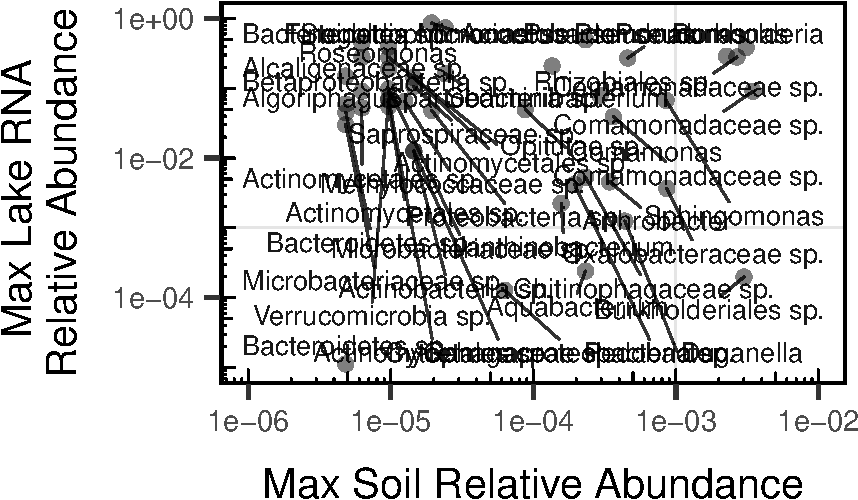
\includegraphics[width=0.7\linewidth]{ReservoirGradient_files/figure-latex/soil_lake_plot-1} \end{center}

\section{Ecosystem Functioning}\label{ecosystem-functioning}

\subsection{Fig 1: Microbial metabolism along reservoir
gradient}\label{fig-1-microbial-metabolism-along-reservoir-gradient}

Read in data

\begin{Shaded}
\begin{Highlighting}[]
\NormalTok{metab <-}\StringTok{ }\KeywordTok{read.table}\NormalTok{(}\StringTok{"data/res.grad.metab.txt"}\NormalTok{, }\DataTypeTok{sep=}\StringTok{"}\CharTok{\textbackslash{}t}\StringTok{"}\NormalTok{, }\DataTypeTok{header=}\OtherTok{TRUE}\NormalTok{)}
\KeywordTok{colnames}\NormalTok{(metab) <-}\StringTok{ }\KeywordTok{c}\NormalTok{(}\StringTok{"dist"}\NormalTok{, }\StringTok{"BP"}\NormalTok{, }\StringTok{"BR"}\NormalTok{)}
\NormalTok{BGE <-}\StringTok{ }\KeywordTok{round}\NormalTok{((metab}\OperatorTok{$}\NormalTok{BP}\OperatorTok{/}\NormalTok{(metab}\OperatorTok{$}\NormalTok{BP }\OperatorTok{+}\StringTok{ }\NormalTok{metab}\OperatorTok{$}\NormalTok{BR)),}\DecValTok{3}\NormalTok{)}
\NormalTok{metab <-}\StringTok{ }\KeywordTok{cbind}\NormalTok{(metab, BGE)}


\CommentTok{# Quadratic regression for BP}
\NormalTok{dist <-}\StringTok{ }\NormalTok{metab}\OperatorTok{$}\NormalTok{dist}
\NormalTok{dist2 <-}\StringTok{ }\NormalTok{metab}\OperatorTok{$}\NormalTok{dist}\OperatorTok{^}\DecValTok{2}
\NormalTok{BP.fit <-}\StringTok{ }\KeywordTok{lm}\NormalTok{(metab}\OperatorTok{$}\NormalTok{BP }\OperatorTok{~}\StringTok{ }\NormalTok{dist }\OperatorTok{+}\StringTok{ }\NormalTok{dist2)}
\NormalTok{BP.R2 <-}\StringTok{ }\KeywordTok{round}\NormalTok{(}\KeywordTok{summary}\NormalTok{(BP.fit)}\OperatorTok{$}\NormalTok{r.squared, }\DecValTok{2}\NormalTok{)}

\CommentTok{# Simple linear regression for BR}
\NormalTok{BR.fit <-}\StringTok{ }\KeywordTok{lm}\NormalTok{(metab}\OperatorTok{$}\NormalTok{BR }\OperatorTok{~}\StringTok{ }\NormalTok{metab}\OperatorTok{$}\NormalTok{dist)}
\NormalTok{BR.R2 <-}\StringTok{ }\KeywordTok{round}\NormalTok{(}\KeywordTok{summary}\NormalTok{(BR.fit)}\OperatorTok{$}\NormalTok{r.squared, }\DecValTok{2}\NormalTok{)}
\NormalTok{BR.int <-}\StringTok{ }\NormalTok{BR.fit}\OperatorTok{$}\NormalTok{coefficients[}\DecValTok{1}\NormalTok{]}
\NormalTok{BR.slp <-}\StringTok{ }\NormalTok{BR.fit}\OperatorTok{$}\NormalTok{coefficients[}\DecValTok{2}\NormalTok{]}

\CommentTok{# Simple linear regression for BGE}
\NormalTok{BGE.fit <-}\StringTok{ }\KeywordTok{lm}\NormalTok{(metab}\OperatorTok{$}\NormalTok{BGE }\OperatorTok{~}\StringTok{ }\NormalTok{metab}\OperatorTok{$}\NormalTok{dist)}
\NormalTok{BGE.R2 <-}\StringTok{ }\KeywordTok{round}\NormalTok{(}\KeywordTok{summary}\NormalTok{(BGE.fit)}\OperatorTok{$}\NormalTok{r.squared, }\DecValTok{2}\NormalTok{)}
\NormalTok{BGE.int <-}\StringTok{ }\NormalTok{BGE.fit}\OperatorTok{$}\NormalTok{coefficients[}\DecValTok{1}\NormalTok{]}
\NormalTok{BGE.slp <-}\StringTok{ }\NormalTok{BGE.fit}\OperatorTok{$}\NormalTok{coefficients[}\DecValTok{2}\NormalTok{]}

\NormalTok{BP.R2}
\NormalTok{BR.R2}
\NormalTok{BGE.R2}

\NormalTok{BP.plot <-}\StringTok{ }\KeywordTok{ggplot}\NormalTok{(metab, }\KeywordTok{aes}\NormalTok{(}\DataTypeTok{x =}\NormalTok{ dist, }\DataTypeTok{y =}\NormalTok{ BP)) }\OperatorTok{+}\StringTok{ }
\StringTok{  }\KeywordTok{geom_point}\NormalTok{() }\OperatorTok{+}\StringTok{ }
\StringTok{  }\KeywordTok{geom_smooth}\NormalTok{(}\DataTypeTok{method =} \StringTok{"lm"}\NormalTok{, }\DataTypeTok{formula =}\NormalTok{ y }\OperatorTok{~}\StringTok{ }\NormalTok{x }\OperatorTok{+}\StringTok{ }\KeywordTok{I}\NormalTok{(x}\OperatorTok{^}\DecValTok{2}\NormalTok{), }\DataTypeTok{color =} \StringTok{"black"}\NormalTok{) }\OperatorTok{+}
\StringTok{  }\KeywordTok{annotate}\NormalTok{(}\DataTypeTok{geom =} \StringTok{"text"}\NormalTok{, }\DataTypeTok{x =} \DecValTok{50}\NormalTok{, }\DataTypeTok{y =} \FloatTok{1.5}\NormalTok{, }\DataTypeTok{size =} \DecValTok{5}\NormalTok{, }\DataTypeTok{label =} \KeywordTok{paste0}\NormalTok{(}\StringTok{"R^2== "}\NormalTok{,BP.R2), }\DataTypeTok{parse =}\NormalTok{ T) }\OperatorTok{+}
\StringTok{  }\KeywordTok{labs}\NormalTok{(}\DataTypeTok{y =} \KeywordTok{expression}\NormalTok{(}\KeywordTok{paste}\NormalTok{(}\StringTok{'BP ('}\NormalTok{, mu ,}\StringTok{'M C h'}\OperatorTok{^-}\DecValTok{1}\OperatorTok{*}\StringTok{ ')'}\NormalTok{)), }
       \DataTypeTok{x =}\NormalTok{ (}\KeywordTok{expression}\NormalTok{(}\StringTok{"Soil"} \OperatorTok\StringTok{ "Riverine"} \OperatorTok\StringTok{ "Lacustrine"} \OperatorTok\StringTok{ "Dam (m)"}\NormalTok{))) }\OperatorTok{+}
\StringTok{  }\KeywordTok{scale_x_reverse}\NormalTok{(}\DataTypeTok{limits =} \KeywordTok{c}\NormalTok{(}\DecValTok{400}\NormalTok{,}\DecValTok{0}\NormalTok{))}
\NormalTok{BR.plot <-}\StringTok{ }\KeywordTok{ggplot}\NormalTok{(metab, }\KeywordTok{aes}\NormalTok{(}\DataTypeTok{x =}\NormalTok{ dist, }\DataTypeTok{y =}\NormalTok{ BR)) }\OperatorTok{+}\StringTok{ }
\StringTok{  }\KeywordTok{geom_point}\NormalTok{() }\OperatorTok{+}\StringTok{ }
\StringTok{  }\KeywordTok{geom_smooth}\NormalTok{(}\DataTypeTok{method =} \StringTok{"lm"}\NormalTok{, }\DataTypeTok{formula =}\NormalTok{ y }\OperatorTok{~}\StringTok{ }\NormalTok{x, }\DataTypeTok{color =} \StringTok{"black"}\NormalTok{) }\OperatorTok{+}\StringTok{ }
\StringTok{  }\KeywordTok{annotate}\NormalTok{(}\StringTok{"text"}\NormalTok{, }\DataTypeTok{x =} \DecValTok{50}\NormalTok{, }\DataTypeTok{y =} \FloatTok{1.5}\NormalTok{, }\DataTypeTok{size =} \DecValTok{5}\NormalTok{, }\DataTypeTok{label =} \KeywordTok{paste0}\NormalTok{(}\StringTok{"R^2== "}\NormalTok{,BR.R2), }\DataTypeTok{parse =}\NormalTok{ T ) }\OperatorTok{+}
\StringTok{  }\KeywordTok{labs}\NormalTok{(}\DataTypeTok{y =} \KeywordTok{expression}\NormalTok{(}\KeywordTok{paste}\NormalTok{(}\StringTok{'BR ('}\NormalTok{, mu ,}\StringTok{'M C h'}\OperatorTok{^-}\DecValTok{1}\OperatorTok{*}\StringTok{ ')'}\NormalTok{)), }
       \DataTypeTok{x =}\NormalTok{ (}\KeywordTok{expression}\NormalTok{(}\StringTok{"Soil"} \OperatorTok\StringTok{ "Riverine"} \OperatorTok\StringTok{ "Lacustrine"} \OperatorTok\StringTok{ "Dam (m)"}\NormalTok{))) }\OperatorTok{+}
\StringTok{  }\KeywordTok{scale_x_reverse}\NormalTok{(}\DataTypeTok{limits =} \KeywordTok{c}\NormalTok{(}\DecValTok{400}\NormalTok{,}\DecValTok{0}\NormalTok{))}
\NormalTok{BGE.plot <-}\StringTok{ }\KeywordTok{ggplot}\NormalTok{(metab, }\KeywordTok{aes}\NormalTok{(}\DataTypeTok{x =}\NormalTok{ dist, }\DataTypeTok{y =}\NormalTok{ BGE)) }\OperatorTok{+}\StringTok{ }
\StringTok{  }\KeywordTok{geom_point}\NormalTok{() }\OperatorTok{+}\StringTok{ }
\StringTok{  }\KeywordTok{geom_smooth}\NormalTok{(}\DataTypeTok{method =} \StringTok{"lm"}\NormalTok{, }\DataTypeTok{formula =}\NormalTok{ y }\OperatorTok{~}\StringTok{ }\NormalTok{x }\OperatorTok{+}\StringTok{ }\KeywordTok{I}\NormalTok{(x}\OperatorTok{^}\DecValTok{2}\NormalTok{), }\DataTypeTok{color =} \StringTok{"black"}\NormalTok{) }\OperatorTok{+}
\StringTok{  }\KeywordTok{annotate}\NormalTok{(}\StringTok{"text"}\NormalTok{, }\DataTypeTok{x =} \DecValTok{50}\NormalTok{, }\DataTypeTok{y =}\NormalTok{ .}\DecValTok{5}\NormalTok{, }\DataTypeTok{size =} \DecValTok{5}\NormalTok{, }\DataTypeTok{label =} \KeywordTok{paste0}\NormalTok{(}\StringTok{"R^2== "}\NormalTok{,BGE.R2), }\DataTypeTok{parse =}\NormalTok{ T ) }\OperatorTok{+}
\StringTok{  }\KeywordTok{labs}\NormalTok{(}\DataTypeTok{y =} \StringTok{"BGE"}\NormalTok{, }
       \DataTypeTok{x =}\NormalTok{ (}\KeywordTok{expression}\NormalTok{(}\StringTok{"Soil"} \OperatorTok\StringTok{ "Riverine"} \OperatorTok\StringTok{ "Lacustrine"} \OperatorTok\StringTok{ "Dam (m)"}\NormalTok{))) }\OperatorTok{+}
\StringTok{  }\KeywordTok{scale_x_reverse}\NormalTok{(}\DataTypeTok{limits =} \KeywordTok{c}\NormalTok{(}\DecValTok{400}\NormalTok{,}\DecValTok{0}\NormalTok{))}
\KeywordTok{plot_grid}\NormalTok{(BP.plot }\OperatorTok{+}\StringTok{ }\KeywordTok{theme}\NormalTok{(}\DataTypeTok{axis.title.x =} \KeywordTok{element_blank}\NormalTok{(), }\DataTypeTok{axis.text.x =} \KeywordTok{element_blank}\NormalTok{(), }
                          \DataTypeTok{plot.margin =} \KeywordTok{unit}\NormalTok{(}\KeywordTok{c}\NormalTok{(}\DecValTok{1}\NormalTok{, }\DecValTok{1}\NormalTok{, }\OperatorTok{-}\DecValTok{1}\NormalTok{, }\DecValTok{0}\NormalTok{), }\StringTok{"cm"}\NormalTok{)), }
\NormalTok{          BR.plot }\OperatorTok{+}\StringTok{ }\KeywordTok{theme}\NormalTok{(}\DataTypeTok{axis.title.x =} \KeywordTok{element_blank}\NormalTok{(), }\DataTypeTok{axis.text.x =} \KeywordTok{element_blank}\NormalTok{(),}
                          \DataTypeTok{plot.margin =} \KeywordTok{unit}\NormalTok{(}\KeywordTok{c}\NormalTok{(}\OperatorTok{-}\DecValTok{1}\NormalTok{, }\DecValTok{1}\NormalTok{, }\OperatorTok{-}\DecValTok{1}\NormalTok{, }\DecValTok{0}\NormalTok{), }\StringTok{"cm"}\NormalTok{)), }
\NormalTok{          BGE.plot }\OperatorTok{+}\StringTok{ }\KeywordTok{theme}\NormalTok{(}\DataTypeTok{plot.margin =} \KeywordTok{unit}\NormalTok{(}\KeywordTok{c}\NormalTok{(}\OperatorTok{-}\DecValTok{1}\NormalTok{, }\DecValTok{1}\NormalTok{, }\DecValTok{0}\NormalTok{, }\DecValTok{0}\NormalTok{), }\StringTok{"cm"}\NormalTok{)), }\DataTypeTok{align =} \StringTok{"hv"}\NormalTok{, }\DataTypeTok{ncol =} \DecValTok{1}\NormalTok{) }\OperatorTok{+}\StringTok{ }
\StringTok{  }\KeywordTok{ggsave}\NormalTok{(}\StringTok{"figures/06_ecosystem-functions.pdf"}\NormalTok{, }\DataTypeTok{bg =} \StringTok{"white"}\NormalTok{, }\DataTypeTok{width =} \DecValTok{6}\NormalTok{, }\DataTypeTok{height =} \DecValTok{11}\NormalTok{)}
\end{Highlighting}
\end{Shaded}

\begin{center}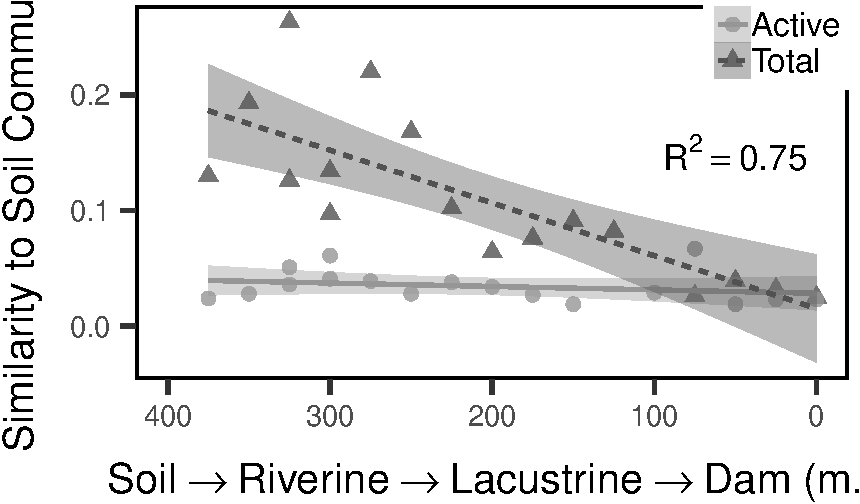
\includegraphics[width=0.7\linewidth]{ReservoirGradient_files/figure-latex/unnamed-chunk-7-1} \end{center}

\subsection{Relation of ecosystem functions and community
structure}\label{relation-of-ecosystem-functions-and-community-structure}

\begin{Shaded}
\begin{Highlighting}[]
\CommentTok{# detrend the spatial signal}
\NormalTok{bp.resid <-}\StringTok{ }\KeywordTok{resid}\NormalTok{(}\KeywordTok{lm}\NormalTok{(BP }\OperatorTok{~}\StringTok{ }\NormalTok{dist }\OperatorTok{+}\StringTok{ }\KeywordTok{I}\NormalTok{(dist)}\OperatorTok{^}\DecValTok{2}\NormalTok{, }\DataTypeTok{data =}\NormalTok{ metab))}
\NormalTok{br.resid <-}\StringTok{ }\KeywordTok{resid}\NormalTok{(}\KeywordTok{lm}\NormalTok{(BR }\OperatorTok{~}\StringTok{ }\NormalTok{dist, }\DataTypeTok{data =}\NormalTok{ metab))}


\NormalTok{metab.resids <-}\StringTok{ }\NormalTok{metab}
\NormalTok{metab.resids}\OperatorTok{$}\NormalTok{BR_resid <-}\StringTok{ }\NormalTok{br.resid }\OperatorTok{+}\StringTok{ }\KeywordTok{mean}\NormalTok{(metab}\OperatorTok{$}\NormalTok{BR)}
\NormalTok{metab.resids}\OperatorTok{$}\NormalTok{BP_resid <-}\StringTok{ }\NormalTok{bp.resid }\OperatorTok{+}\StringTok{ }\KeywordTok{mean}\NormalTok{(metab}\OperatorTok{$}\NormalTok{BP)}

\NormalTok{transient.metabolism <-}\StringTok{ }\KeywordTok{data.frame}\NormalTok{(}\DataTypeTok{transients =}\NormalTok{ terr.REL, }\DataTypeTok{dist =}\NormalTok{ design.dna}\OperatorTok{$}\NormalTok{distance) }\OperatorTok\StringTok{ }
\StringTok{  }\KeywordTok{left_join}\NormalTok{(metab.resids) }


\NormalTok{bp.mod.quad <-}\StringTok{ }\KeywordTok{lm}\NormalTok{(BP_resid }\OperatorTok{~}\StringTok{ }\NormalTok{transients }\OperatorTok{+}\StringTok{ }\KeywordTok{I}\NormalTok{(transients}\OperatorTok{^}\DecValTok{2}\NormalTok{), }\DataTypeTok{data =}\NormalTok{ transient.metabolism)}
\NormalTok{bp.mod.lin <-}\StringTok{ }\KeywordTok{lm}\NormalTok{(BP_resid }\OperatorTok{~}\StringTok{ }\NormalTok{transients, }\DataTypeTok{data =}\NormalTok{ transient.metabolism)}
\NormalTok{bp.mod.int <-}\StringTok{ }\KeywordTok{lm}\NormalTok{(BP_resid }\OperatorTok{~}\StringTok{ }\DecValTok{1}\NormalTok{, }\DataTypeTok{data =}\NormalTok{ transient.metabolism)}
\KeywordTok{anova}\NormalTok{(bp.mod.int, bp.mod.lin, bp.mod.quad)}
\KeywordTok{AIC}\NormalTok{(bp.mod.quad, bp.mod.lin, bp.mod.int)}

\NormalTok{br.mod.quad <-}\StringTok{ }\KeywordTok{lm}\NormalTok{(BR_resid }\OperatorTok{~}\StringTok{ }\NormalTok{transients }\OperatorTok{+}\StringTok{ }\KeywordTok{I}\NormalTok{(transients}\OperatorTok{^}\DecValTok{2}\NormalTok{), }\DataTypeTok{data =}\NormalTok{ transient.metabolism)}
\NormalTok{br.mod.lin <-}\StringTok{ }\KeywordTok{lm}\NormalTok{(BR_resid }\OperatorTok{~}\StringTok{ }\NormalTok{transients, }\DataTypeTok{data =}\NormalTok{ transient.metabolism)}
\NormalTok{br.mod.int <-}\StringTok{ }\KeywordTok{lm}\NormalTok{(BR_resid }\OperatorTok{~}\StringTok{ }\DecValTok{1}\NormalTok{, }\DataTypeTok{data =}\NormalTok{ transient.metabolism)}
\KeywordTok{anova}\NormalTok{(br.mod.int, br.mod.lin, br.mod.quad)}
\KeywordTok{AIC}\NormalTok{(br.mod.int, br.mod.lin, br.mod.quad)}

\NormalTok{bge.mod.quad <-}\StringTok{ }\KeywordTok{lm}\NormalTok{(BGE }\OperatorTok{~}\StringTok{ }\NormalTok{transients }\OperatorTok{+}\StringTok{ }\KeywordTok{I}\NormalTok{(transients}\OperatorTok{^}\DecValTok{2}\NormalTok{), }\DataTypeTok{data =}\NormalTok{ transient.metabolism)}
\NormalTok{bge.mod.lin <-}\StringTok{ }\KeywordTok{lm}\NormalTok{(BGE }\OperatorTok{~}\StringTok{ }\NormalTok{transients, }\DataTypeTok{data =}\NormalTok{ transient.metabolism)}
\NormalTok{bge.mod.int <-}\StringTok{ }\KeywordTok{lm}\NormalTok{(BGE }\OperatorTok{~}\StringTok{ }\DecValTok{1}\NormalTok{, }\DataTypeTok{data =}\NormalTok{ transient.metabolism)}
\KeywordTok{anova}\NormalTok{(bge.mod.int, bge.mod.lin, bge.mod.quad)}
\KeywordTok{AIC}\NormalTok{(bge.mod.int, bge.mod.lin, bge.mod.quad)}

\KeywordTok{round}\NormalTok{(}\KeywordTok{summary}\NormalTok{(br.mod.quad)}\OperatorTok{$}\NormalTok{r.squared, }\DecValTok{2}\NormalTok{)}
\KeywordTok{round}\NormalTok{(}\KeywordTok{summary}\NormalTok{(bp.mod.quad)}\OperatorTok{$}\NormalTok{r.squared, }\DecValTok{2}\NormalTok{)}


\NormalTok{total_core <-}\StringTok{ }\KeywordTok{rowSums}\NormalTok{(OTUsREL[design}\OperatorTok{$}\NormalTok{molecule }\OperatorTok{==}\StringTok{ "DNA"} \OperatorTok{&}\StringTok{ }\NormalTok{design}\OperatorTok{$}\NormalTok{type }\OperatorTok{==}\StringTok{ "water"}\NormalTok{,}
                               \KeywordTok{subset}\NormalTok{(}\KeywordTok{rbind.data.frame}\NormalTok{(high.activity.water.core, }
\NormalTok{                                                       high.activity.soil.core), RNA.max }\OperatorTok{>}\StringTok{ }\NormalTok{.}\DecValTok{01}\NormalTok{)}\OperatorTok{$}\NormalTok{OTU])}

\KeywordTok{summary}\NormalTok{(}\KeywordTok{lm}\NormalTok{(BP }\OperatorTok{~}\StringTok{ }\NormalTok{transients }\OperatorTok{*}\StringTok{ }\NormalTok{dist, transient.metabolism))}
\KeywordTok{summary}\NormalTok{(}\KeywordTok{lm}\NormalTok{(BR }\OperatorTok{~}\StringTok{ }\NormalTok{transients }\OperatorTok{*}\StringTok{ }\NormalTok{dist, transient.metabolism))}


\KeywordTok{data.frame}\NormalTok{(}
  \DataTypeTok{soil_core =} \KeywordTok{rowSums}\NormalTok{(OTUsREL[design}\OperatorTok{$}\NormalTok{molecule }\OperatorTok{==}\StringTok{ "DNA"} \OperatorTok{&}\StringTok{ }\NormalTok{design}\OperatorTok{$}\NormalTok{type }\OperatorTok{==}\StringTok{ "water"}\NormalTok{,}
           \KeywordTok{subset}\NormalTok{(soil.vs.lake.abunds, RNA.max }\OperatorTok{>}\StringTok{ }\NormalTok{.}\DecValTok{01}\NormalTok{)}\OperatorTok{$}\NormalTok{OTU]), }
  \DataTypeTok{dist =}\NormalTok{ design.dna}\OperatorTok{$}\NormalTok{distance) }\OperatorTok\StringTok{ }
\StringTok{  }\KeywordTok{left_join}\NormalTok{(metab.resids) }\OperatorTok\StringTok{ }\KeywordTok{select}\NormalTok{(}\OperatorTok{-}\NormalTok{BGE, }\OperatorTok{-}\NormalTok{BP, }\OperatorTok{-}\NormalTok{BR) }\OperatorTok\StringTok{ }\KeywordTok{gather}\NormalTok{(metab, value, }\OperatorTok{-}\NormalTok{soil_core, }\OperatorTok{-}\NormalTok{dist) }\OperatorTok\StringTok{ }
\StringTok{  }\KeywordTok{ggplot}\NormalTok{(}\KeywordTok{aes}\NormalTok{(}\DataTypeTok{x =}\NormalTok{ soil_core, }\DataTypeTok{y =}\NormalTok{ value, }\DataTypeTok{color =}\NormalTok{ metab, }\DataTypeTok{fill =}\NormalTok{ metab)) }\OperatorTok{+}
\StringTok{  }\KeywordTok{geom_point}\NormalTok{(}\DataTypeTok{size =} \DecValTok{2}\NormalTok{) }\OperatorTok{+}\StringTok{ }
\StringTok{  }\KeywordTok{geom_smooth}\NormalTok{(}\DataTypeTok{alpha =}\NormalTok{ .}\DecValTok{25}\NormalTok{, }\DataTypeTok{method =} \StringTok{'lm'}\NormalTok{, }\DataTypeTok{formula =}\NormalTok{ y }\OperatorTok{~}\StringTok{ }\NormalTok{x }\OperatorTok{+}\StringTok{ }\KeywordTok{I}\NormalTok{(x}\OperatorTok{^}\DecValTok{2}\NormalTok{)) }\OperatorTok{+}
\StringTok{  }\KeywordTok{labs}\NormalTok{(}\DataTypeTok{x =} \StringTok{"Relative Abundance of Soil-derived Core"}\NormalTok{,}
       \DataTypeTok{y =} \KeywordTok{expression}\NormalTok{(}\KeywordTok{paste}\NormalTok{(}\StringTok{'Metabolism ('}\NormalTok{, mu ,}\StringTok{'M C h'}\OperatorTok{^-}\DecValTok{1}\OperatorTok{*}\StringTok{ ')'}\NormalTok{))) }\OperatorTok{+}
\StringTok{  }\KeywordTok{scale_color_viridis}\NormalTok{(}\StringTok{"Ecosystem Function"}\NormalTok{, }\DataTypeTok{discrete =}\NormalTok{ T, }\DataTypeTok{begin =}\NormalTok{ .}\DecValTok{1}\NormalTok{, }\DataTypeTok{end =}\NormalTok{ .}\DecValTok{6}\NormalTok{, }\DataTypeTok{option =} \StringTok{"D"}\NormalTok{) }\OperatorTok{+}
\StringTok{  }\KeywordTok{scale_fill_viridis}\NormalTok{(}\StringTok{"Ecosystem Function"}\NormalTok{, }\DataTypeTok{discrete =}\NormalTok{ T, }\DataTypeTok{begin =}\NormalTok{ .}\DecValTok{1}\NormalTok{, }\DataTypeTok{end =}\NormalTok{ .}\DecValTok{6}\NormalTok{, }\DataTypeTok{option =} \StringTok{"D"}\NormalTok{) }\OperatorTok{+}
\StringTok{  }\KeywordTok{ggsave}\NormalTok{(}\StringTok{"figures/06_soilcore-function.pdf"}\NormalTok{, }\DataTypeTok{bg =} \StringTok{"white"}\NormalTok{, }\DataTypeTok{width =} \DecValTok{7}\NormalTok{, }\DataTypeTok{height =} \DecValTok{6}\NormalTok{)}

\KeywordTok{data.frame}\NormalTok{(}
  \DataTypeTok{water_core =} \KeywordTok{rowSums}\NormalTok{(OTUsREL[design}\OperatorTok{$}\NormalTok{molecule }\OperatorTok{==}\StringTok{ "DNA"} \OperatorTok{&}\StringTok{ }\NormalTok{design}\OperatorTok{$}\NormalTok{type }\OperatorTok{==}\StringTok{ "water"}\NormalTok{,}
                               \KeywordTok{subset}\NormalTok{(high.activity.water.core, RNA.max }\OperatorTok{>}\StringTok{ }\NormalTok{.}\DecValTok{01}\NormalTok{)}\OperatorTok{$}\NormalTok{OTU]), }
  \DataTypeTok{dist =}\NormalTok{ design.dna}\OperatorTok{$}\NormalTok{distance) }\OperatorTok\StringTok{ }
\StringTok{  }\KeywordTok{left_join}\NormalTok{(metab.resids) }\OperatorTok\StringTok{ }\KeywordTok{select}\NormalTok{(}\OperatorTok{-}\NormalTok{BGE,}\OperatorTok{-}\NormalTok{BR,}\OperatorTok{-}\NormalTok{BP) }\OperatorTok\StringTok{ }\KeywordTok{gather}\NormalTok{(metab, value, }\OperatorTok{-}\NormalTok{water_core, }\OperatorTok{-}\NormalTok{dist) }\OperatorTok\StringTok{ }
\StringTok{  }\KeywordTok{ggplot}\NormalTok{(}\KeywordTok{aes}\NormalTok{(}\DataTypeTok{x =}\NormalTok{ water_core, }\DataTypeTok{y =}\NormalTok{ value, }\DataTypeTok{color =}\NormalTok{ metab, }\DataTypeTok{fill =}\NormalTok{ metab)) }\OperatorTok{+}
\StringTok{  }\KeywordTok{geom_point}\NormalTok{(}\DataTypeTok{size =} \DecValTok{2}\NormalTok{) }\OperatorTok{+}\StringTok{ }
\StringTok{  }\KeywordTok{geom_smooth}\NormalTok{(}\DataTypeTok{alpha =}\NormalTok{ .}\DecValTok{25}\NormalTok{, }\DataTypeTok{method =} \StringTok{'lm'}\NormalTok{, }\DataTypeTok{formula =}\NormalTok{ y }\OperatorTok{~}\StringTok{ }\NormalTok{x }\OperatorTok{+}\StringTok{ }\KeywordTok{I}\NormalTok{(x}\OperatorTok{^}\DecValTok{2}\NormalTok{)) }\OperatorTok{+}
\StringTok{  }\KeywordTok{labs}\NormalTok{(}\DataTypeTok{x =} \StringTok{"Relative Abundance of non-soil-derived Core"}\NormalTok{,}
       \DataTypeTok{y =} \KeywordTok{expression}\NormalTok{(}\KeywordTok{paste}\NormalTok{(}\StringTok{'Metabolism ('}\NormalTok{, mu ,}\StringTok{'M C h'}\OperatorTok{^-}\DecValTok{1}\OperatorTok{*}\StringTok{ ')'}\NormalTok{))) }\OperatorTok{+}
\StringTok{  }\KeywordTok{scale_color_viridis}\NormalTok{(}\StringTok{"Ecosystem Function"}\NormalTok{, }\DataTypeTok{discrete =}\NormalTok{ T, }\DataTypeTok{begin =}\NormalTok{ .}\DecValTok{1}\NormalTok{, }\DataTypeTok{end =}\NormalTok{ .}\DecValTok{6}\NormalTok{, }\DataTypeTok{option =} \StringTok{"D"}\NormalTok{) }\OperatorTok{+}
\StringTok{  }\KeywordTok{scale_fill_viridis}\NormalTok{(}\StringTok{"Ecosystem Function"}\NormalTok{, }\DataTypeTok{discrete =}\NormalTok{ T, }\DataTypeTok{begin =}\NormalTok{ .}\DecValTok{1}\NormalTok{, }\DataTypeTok{end =}\NormalTok{ .}\DecValTok{6}\NormalTok{, }\DataTypeTok{option =} \StringTok{"D"}\NormalTok{) }\OperatorTok{+}
\StringTok{  }\KeywordTok{ggsave}\NormalTok{(}\StringTok{"figures/06_nonsoilcore-function.pdf"}\NormalTok{, }\DataTypeTok{bg =} \StringTok{"white"}\NormalTok{, }\DataTypeTok{width =} \DecValTok{7}\NormalTok{, }\DataTypeTok{height =} \DecValTok{6}\NormalTok{)}



\KeywordTok{data.frame}\NormalTok{(}\DataTypeTok{transients =} \KeywordTok{resid}\NormalTok{(}\KeywordTok{lm}\NormalTok{(terr.REL }\OperatorTok{~}\StringTok{ }\NormalTok{design.dna}\OperatorTok{$}\NormalTok{distance)) }\OperatorTok{+}\StringTok{ }\KeywordTok{mean}\NormalTok{(terr.REL), }\DataTypeTok{dist =}\NormalTok{ design.dna}\OperatorTok{$}\NormalTok{distance) }\OperatorTok\StringTok{ }
\StringTok{  }\KeywordTok{left_join}\NormalTok{(metab.resids) }\OperatorTok\StringTok{ }\KeywordTok{select}\NormalTok{(}\OperatorTok{-}\NormalTok{BGE, }\OperatorTok{-}\NormalTok{BP, }\OperatorTok{-}\NormalTok{BR) }\OperatorTok\StringTok{ }\KeywordTok{gather}\NormalTok{(metab, value, }\OperatorTok{-}\NormalTok{transients, }\OperatorTok{-}\NormalTok{dist) }\OperatorTok\StringTok{ }
\StringTok{  }\KeywordTok{ggplot}\NormalTok{(}\KeywordTok{aes}\NormalTok{(}\DataTypeTok{x =}\NormalTok{ transients, }\DataTypeTok{y =}\NormalTok{ value, }\DataTypeTok{color =}\NormalTok{ metab, }\DataTypeTok{fill =}\NormalTok{ metab)) }\OperatorTok{+}
\StringTok{  }\KeywordTok{geom_point}\NormalTok{(}\DataTypeTok{size =} \DecValTok{2}\NormalTok{, }\DataTypeTok{show.legend =}\NormalTok{ F) }\OperatorTok{+}\StringTok{ }
\StringTok{  }\KeywordTok{geom_smooth}\NormalTok{(}\DataTypeTok{alpha =}\NormalTok{ .}\DecValTok{25}\NormalTok{, }\DataTypeTok{method =} \StringTok{'lm'}\NormalTok{, }\DataTypeTok{formula =}\NormalTok{ y }\OperatorTok{~}\StringTok{ }\NormalTok{x, }\DataTypeTok{show.legend =}\NormalTok{ F) }\OperatorTok{+}
\StringTok{  }\KeywordTok{annotation_logticks}\NormalTok{(}\DataTypeTok{sides =} \StringTok{"b"}\NormalTok{) }\OperatorTok{+}
\StringTok{  }\KeywordTok{labs}\NormalTok{(}\DataTypeTok{x =} \StringTok{"Relative Abundance of Transient Taxa"}\NormalTok{,}
       \DataTypeTok{y =} \KeywordTok{expression}\NormalTok{(}\KeywordTok{paste}\NormalTok{(}\StringTok{'Metabolism ('}\NormalTok{, mu ,}\StringTok{'M C h'}\OperatorTok{^-}\DecValTok{1}\OperatorTok{*}\StringTok{ ')'}\NormalTok{))) }\OperatorTok{+}
\StringTok{  }\KeywordTok{scale_color_viridis}\NormalTok{(}\StringTok{"Ecosystem Function"}\NormalTok{, }\DataTypeTok{discrete =}\NormalTok{ T, }\DataTypeTok{begin =}\NormalTok{ .}\DecValTok{1}\NormalTok{, }\DataTypeTok{end =}\NormalTok{ .}\DecValTok{6}\NormalTok{, }\DataTypeTok{option =} \StringTok{"D"}\NormalTok{) }\OperatorTok{+}
\StringTok{  }\KeywordTok{scale_fill_viridis}\NormalTok{(}\StringTok{"Ecosystem Function"}\NormalTok{, }\DataTypeTok{discrete =}\NormalTok{ T, }\DataTypeTok{begin =}\NormalTok{ .}\DecValTok{1}\NormalTok{, }\DataTypeTok{end =}\NormalTok{ .}\DecValTok{6}\NormalTok{, }\DataTypeTok{option =} \StringTok{"D"}\NormalTok{) }\OperatorTok{+}
\StringTok{  }\KeywordTok{scale_y_continuous}\NormalTok{(}\DataTypeTok{limits =} \KeywordTok{c}\NormalTok{(}\DecValTok{0}\NormalTok{,}\DecValTok{3}\NormalTok{)) }\OperatorTok{+}
\StringTok{  }\KeywordTok{theme}\NormalTok{(}\DataTypeTok{plot.margin =} \KeywordTok{unit}\NormalTok{(}\KeywordTok{c}\NormalTok{(}\DecValTok{1}\NormalTok{,}\DecValTok{1}\NormalTok{,}\DecValTok{0}\NormalTok{,}\DecValTok{0}\NormalTok{), }\StringTok{"cm"}\NormalTok{)) }\OperatorTok{+}
\StringTok{  }\KeywordTok{ggsave}\NormalTok{(}\StringTok{"figures/06_transients-function.pdf"}\NormalTok{, }\DataTypeTok{bg =} \StringTok{"white"}\NormalTok{, }\DataTypeTok{width =} \DecValTok{7}\NormalTok{, }\DataTypeTok{height =} \DecValTok{6}\NormalTok{)}


\NormalTok{core.metab <-}\StringTok{ }\KeywordTok{data.frame}\NormalTok{(}
  \DataTypeTok{total_core =} \KeywordTok{rowSums}\NormalTok{(OTUsREL[design}\OperatorTok{$}\NormalTok{molecule }\OperatorTok{==}\StringTok{ "DNA"} \OperatorTok{&}\StringTok{ }\NormalTok{design}\OperatorTok{$}\NormalTok{type }\OperatorTok{==}\StringTok{ "water"}\NormalTok{,}
                               \KeywordTok{subset}\NormalTok{(}\KeywordTok{rbind.data.frame}\NormalTok{(high.activity.water.core, }
\NormalTok{                                                       high.activity.soil.core), RNA.max }\OperatorTok{>}\StringTok{ }\NormalTok{.}\DecValTok{01}\NormalTok{)}\OperatorTok{$}\NormalTok{OTU]), }
  \DataTypeTok{dist =}\NormalTok{ design.dna}\OperatorTok{$}\NormalTok{distance) }\OperatorTok\StringTok{ }
\StringTok{  }\KeywordTok{left_join}\NormalTok{(metab.resids)}

\KeywordTok{summary}\NormalTok{(}\KeywordTok{lm}\NormalTok{(BP }\OperatorTok{~}\StringTok{ }\NormalTok{total_core }\OperatorTok{*}\StringTok{ }\NormalTok{dist, core.metab))}
\KeywordTok{summary}\NormalTok{(}\KeywordTok{lm}\NormalTok{(BR }\OperatorTok{~}\StringTok{ }\NormalTok{total_core }\OperatorTok{+}\StringTok{ }\NormalTok{dist, core.metab))}


\NormalTok{core.metab <-}\StringTok{ }\KeywordTok{data.frame}\NormalTok{(}
  \DataTypeTok{total_core =} \KeywordTok{rowSums}\NormalTok{(OTUsREL[design}\OperatorTok{$}\NormalTok{molecule }\OperatorTok{==}\StringTok{ "DNA"} \OperatorTok{&}\StringTok{ }\NormalTok{design}\OperatorTok{$}\NormalTok{type }\OperatorTok{==}\StringTok{ "water"}\NormalTok{,}
                               \KeywordTok{subset}\NormalTok{(}\KeywordTok{rbind.data.frame}\NormalTok{(high.activity.water.core, }
\NormalTok{                                                       high.activity.soil.core), RNA.max }\OperatorTok{>}\StringTok{ }\NormalTok{.}\DecValTok{01}\NormalTok{)}\OperatorTok{$}\NormalTok{OTU]), }
  \DataTypeTok{dist =}\NormalTok{ design.dna}\OperatorTok{$}\NormalTok{distance) }\OperatorTok\StringTok{ }
\StringTok{  }\KeywordTok{left_join}\NormalTok{(metab.resids)}
\NormalTok{core.metab}\OperatorTok{$}\NormalTok{total_core_resid <-}\StringTok{ }\KeywordTok{resid}\NormalTok{(}\KeywordTok{lm}\NormalTok{(total_core }\OperatorTok{~}\StringTok{ }\NormalTok{dist }\OperatorTok{+}\StringTok{ }\KeywordTok{I}\NormalTok{(dist}\OperatorTok{^}\DecValTok{2}\NormalTok{), core.metab)) }\OperatorTok{+}\StringTok{ }\KeywordTok{mean}\NormalTok{(core.metab}\OperatorTok{$}\NormalTok{total_core)}
\KeywordTok{summary}\NormalTok{(}\KeywordTok{lm}\NormalTok{(BP_resid }\OperatorTok{~}\StringTok{ }\NormalTok{total_core, core.metab))}
\KeywordTok{summary}\NormalTok{(}\KeywordTok{lm}\NormalTok{(BR_resid }\OperatorTok{~}\StringTok{ }\NormalTok{total_core }\OperatorTok{+}\StringTok{ }\KeywordTok{I}\NormalTok{(total_core}\OperatorTok{^}\DecValTok{2}\NormalTok{), core.metab))}


\NormalTok{core.metab }\OperatorTok\StringTok{ }\KeywordTok{select}\NormalTok{(}\OperatorTok{-}\NormalTok{BGE, }\OperatorTok{-}\NormalTok{BP, }\OperatorTok{-}\NormalTok{BR, }\OperatorTok{-}\NormalTok{total_core) }\OperatorTok\StringTok{ }\KeywordTok{gather}\NormalTok{(metab, value, }\OperatorTok{-}\NormalTok{total_core_resid, }\OperatorTok{-}\NormalTok{dist) }\OperatorTok\StringTok{ }
\StringTok{  }\KeywordTok{ggplot}\NormalTok{(}\KeywordTok{aes}\NormalTok{(}\DataTypeTok{x =}\NormalTok{ total_core_resid, }\DataTypeTok{y =}\NormalTok{ value, }\DataTypeTok{color =}\NormalTok{ metab, }\DataTypeTok{fill =}\NormalTok{ metab)) }\OperatorTok{+}
\StringTok{  }\KeywordTok{geom_point}\NormalTok{(}\DataTypeTok{size =} \DecValTok{2}\NormalTok{, }\DataTypeTok{show.legend =}\NormalTok{ F) }\OperatorTok{+}\StringTok{ }
\StringTok{  }\KeywordTok{geom_smooth}\NormalTok{(}\DataTypeTok{alpha =}\NormalTok{ .}\DecValTok{25}\NormalTok{, }\DataTypeTok{method =} \StringTok{'lm'}\NormalTok{, }\DataTypeTok{formula =}\NormalTok{ y }\OperatorTok{~}\StringTok{ }\NormalTok{x, }\DataTypeTok{show.legend =}\NormalTok{ F) }\OperatorTok{+}
\StringTok{  }\KeywordTok{labs}\NormalTok{(}\DataTypeTok{x =} \StringTok{"Relative Abundance of Core Taxa"}\NormalTok{,}
       \DataTypeTok{y =} \KeywordTok{expression}\NormalTok{(}\KeywordTok{paste}\NormalTok{(}\StringTok{'Metabolism ('}\NormalTok{, mu ,}\StringTok{'M C h'}\OperatorTok{^-}\DecValTok{1}\OperatorTok{*}\StringTok{ ')'}\NormalTok{))) }\OperatorTok{+}
\StringTok{  }\KeywordTok{scale_color_viridis}\NormalTok{(}\StringTok{"Ecosystem Function"}\NormalTok{, }\DataTypeTok{discrete =}\NormalTok{ T, }\DataTypeTok{begin =}\NormalTok{ .}\DecValTok{1}\NormalTok{, }\DataTypeTok{end =}\NormalTok{ .}\DecValTok{6}\NormalTok{, }\DataTypeTok{option =} \StringTok{"D"}\NormalTok{) }\OperatorTok{+}
\StringTok{  }\KeywordTok{scale_fill_viridis}\NormalTok{(}\StringTok{"Ecosystem Function"}\NormalTok{, }\DataTypeTok{discrete =}\NormalTok{ T, }\DataTypeTok{begin =}\NormalTok{ .}\DecValTok{1}\NormalTok{, }\DataTypeTok{end =}\NormalTok{ .}\DecValTok{6}\NormalTok{, }\DataTypeTok{option =} \StringTok{"D"}\NormalTok{) }\OperatorTok{+}
\StringTok{  }\KeywordTok{scale_y_continuous}\NormalTok{(}\DataTypeTok{limits =} \KeywordTok{c}\NormalTok{(}\DecValTok{0}\NormalTok{,}\DecValTok{3}\NormalTok{)) }\OperatorTok{+}
\StringTok{  }\KeywordTok{theme}\NormalTok{(}\DataTypeTok{plot.margin =} \KeywordTok{unit}\NormalTok{(}\KeywordTok{c}\NormalTok{(}\DecValTok{1}\NormalTok{,}\DecValTok{1}\NormalTok{,}\DecValTok{0}\NormalTok{,}\DecValTok{0}\NormalTok{), }\StringTok{"cm"}\NormalTok{)) }\OperatorTok{+}
\StringTok{  }\KeywordTok{ggsave}\NormalTok{(}\StringTok{"figures/06_core-function.pdf"}\NormalTok{, }\DataTypeTok{bg =} \StringTok{"white"}\NormalTok{, }\DataTypeTok{width =} \DecValTok{7}\NormalTok{, }\DataTypeTok{height =} \DecValTok{6}\NormalTok{)}
\end{Highlighting}
\end{Shaded}

\section{Analyze environmental
controls}\label{analyze-environmental-controls}

\begin{Shaded}
\begin{Highlighting}[]
\CommentTok{# library(AEM)}
\CommentTok{# # pull out the in-lake samples}
\CommentTok{# in.lake.dna.samples <- which(design$type == "water" & design$molecule == "DNA" & design$distance < 300)}
\CommentTok{# env <- env.dat[which(env.dat$sample.ID %in% design$station[in.lake.dna.samples]),c("temp", "pH", "DO", "TP", "chla")]}
\CommentTok{# env <- scale(env)}
\CommentTok{# geo_dist <- as.vector(dist(design[in.lake.dna.samples,]$distance))}
\CommentTok{# env_dist <- as.vector(dist(env))}
\CommentTok{# com_dist <- as.vector(vegdist(decostand(lake.tot, "total")))}
\CommentTok{# data.frame(env_dist = resid(lm(env_dist ~ geo_dist)), }
\CommentTok{#            com_dist = com_dist,}
\CommentTok{#            geo_dist = resid(lm(geo_dist ~ env_dist))) %>% }
\CommentTok{#   ggplot(aes(x = env_dist, y = com_dist)) + }
\CommentTok{#   geom_point(alpha = 0.5) + }
\CommentTok{#   geom_smooth(method = 'lm')}
\CommentTok{# data.frame(env_dist = resid(lm(env_dist ~ geo_dist)), }
\CommentTok{#            com_dist = com_dist,}
\CommentTok{#            geo_dist = resid(lm(geo_dist ~ env_dist))) %>% }
\CommentTok{#   ggplot(aes(x = geo_dist, y = com_dist)) + }
\CommentTok{#   geom_point(alpha = 0.5) + }
\CommentTok{#   geom_smooth(method = 'lm')}
\CommentTok{# data.frame(env_dist = resid(lm(env_dist ~ geo_dist)), }
\CommentTok{#            com_dist = com_dist,}
\CommentTok{#            geo_dist = resid(lm(geo_dist ~ env_dist))) %>% }
\CommentTok{#   ggplot(aes(x = env_dist, y = geo_dist)) + }
\CommentTok{#   geom_point(alpha = 0.5) + }
\CommentTok{#   geom_smooth(method = 'lm')}
\CommentTok{# }
\CommentTok{# # construct asymetric eigenvector maps along transect}
\CommentTok{# n <- nrow(env)}
\CommentTok{# aem.out <- aem.time(n, moran = T, plot.moran = T)}
\CommentTok{# colnames(aem.out$aem) <- paste0("AEM", seq(1, n-1))}
\CommentTok{# aems <- aem.out$aem[,which(aem.out$Moran$p.value < 0.05)]}
\CommentTok{# }
\CommentTok{# }
\CommentTok{# prcomp(env, scale. = T)}
\CommentTok{# round(cor(cbind(aems, env)),2)}
\CommentTok{# lake.tot <- OTUs[in.lake.dna.samples,]}
\CommentTok{# }
\CommentTok{# vp.tot.pos <- varpart(lake.tot, aems[,c("AEM1", "AEM2", "AEM3")], env, transfo = "hellinger")}
\CommentTok{# vp.tot.pos}
\CommentTok{# plot(vp.tot.pos)}
\CommentTok{# }
\CommentTok{# vp.tot.neg <- varpart(lake.tot, aems[,c("AEM8", "AEM9", "AEM10")], env, transfo = "hellinger")}
\CommentTok{# vp.tot.neg}
\CommentTok{# plot(vp.tot.neg)}
\CommentTok{# }
\CommentTok{# # rna}
\CommentTok{# in.lake.rna.samples <- which(design$type == "water" & design$molecule == "RNA" & design$distance < 300)}
\CommentTok{# env <- env.dat[which(env.dat$sample.ID %in% design$station[in.lake.rna.samples]),c("temp", "pH", "DO", "TP", "chla")]}
\CommentTok{# env <- scale(env)}
\CommentTok{# }
\CommentTok{# # construct asymetric eigenvector maps along transect}
\CommentTok{# n <- nrow(env)}
\CommentTok{# aem.out <- AEM::aem.time(n, moran = T, plot.moran = T)}
\CommentTok{# colnames(aem.out$aem) <- paste0("AEM", seq(1, n-1))}
\CommentTok{# aems <- aem.out$aem[,which(aem.out$Moran$p.value < 0.05)]}
\CommentTok{# }
\CommentTok{# prcomp(env, scale. = T)}
\CommentTok{# round(cor(cbind(aems, env)),2)}
\CommentTok{# lake.act <- OTUs[in.lake.rna.samples,]}
\CommentTok{# }
\CommentTok{# geo_dist <- as.vector(dist(design[in.lake.rna.samples,]$distance))}
\CommentTok{# env_dist <- as.vector(dist(env))}
\CommentTok{# com_dist <- as.vector(vegdist(decostand(lake.act, "total")))}
\CommentTok{# data.frame(env_dist = resid(lm(env_dist ~ geo_dist)), }
\CommentTok{#            com_dist = com_dist,}
\CommentTok{#            geo_dist = resid(lm(geo_dist ~ env_dist))) %>% }
\CommentTok{#   ggplot(aes(x = env_dist, y = com_dist)) + }
\CommentTok{#   geom_point(alpha = 0.5) + }
\CommentTok{#   geom_smooth(method = 'lm')}
\CommentTok{# data.frame(env_dist = resid(lm(env_dist ~ geo_dist)), }
\CommentTok{#            com_dist = com_dist,}
\CommentTok{#            geo_dist = resid(lm(geo_dist ~ env_dist))) %>% }
\CommentTok{#   ggplot(aes(x = geo_dist, y = com_dist)) + }
\CommentTok{#   geom_point(alpha = 0.5) + }
\CommentTok{#   geom_smooth(method = 'lm')}
\CommentTok{# data.frame(env_dist = resid(lm(env_dist ~ geo_dist)), }
\CommentTok{#            com_dist = com_dist,}
\CommentTok{#            geo_dist = resid(lm(geo_dist ~ env_dist))) %>% }
\CommentTok{#   ggplot(aes(x = env_dist, y = geo_dist)) + }
\CommentTok{#   geom_point(alpha = 0.5) + }
\CommentTok{#   geom_smooth(method = 'lm')}
\CommentTok{# }
\CommentTok{# vp.act.pos <- varpart(lake.act, aems[,c("AEM1", "AEM2", "AEM3")], env, transfo = "hellinger")}
\CommentTok{# vp.act.pos}
\CommentTok{# plot(vp.act.pos)}
\CommentTok{# }
\CommentTok{# vp.act.neg <- varpart(lake.act, aems[,c("AEM8", "AEM9", "AEM10")], env, transfo = "hellinger")}
\CommentTok{# vp.act.neg}
\CommentTok{# plot(vp.act.neg)}
\end{Highlighting}
\end{Shaded}


\end{document}
